\documentclass[12pt,a4paper]{article}

% Prefer ignored local data; fall back to the tracked non-sensitive example.
\IfFileExists{config/datos.local.tex}{\input{config/datos.local.tex}}{% Tracked, non-sensitive data template for local document customization.
% Copy this file to config/datos.local.tex and replace the placeholders.
% Active entry points load datos.local.tex when it exists; otherwise they
% load this example so the source remains structurally complete.

\newcommand{\PracticanteNombre}{Nombre del practicante}
\newcommand{\PracticanteCodigo}{CÓDIGO}
\newcommand{\PracticanteEspecialidad}{Ingeniería de Software}
\newcommand{\PracticanteFacultad}{FIMEES}
\newcommand{\PracticantePromocion}{AÑO}
\newcommand{\InstitucionNombre}{Dirección de Proyección Social y Extensión Cultural}
\newcommand{\InstitucionOficina}{Oficina de Dirección de Proyección Social y Extensión Cultural}
\newcommand{\InstitucionJefa}{Nombre de la jefa de la unidad receptora}
\newcommand{\DocenteNombre}{Nombre del docente de prácticas}
\newcommand{\FechaInicio}{DD/MM/AAAA}
\newcommand{\FechaFin}{DD/MM/AAAA}
\newcommand{\CentroDireccion}{Dirección del centro de prácticas}
\newcommand{\TelefonoMelissa}{Teléfono de contacto del proyecto}
\newcommand{\TelefonoJefa}{Teléfono de la dirección}
\newcommand{\TelefonoOficina}{Teléfono de la oficina}
\newcommand{\SitioWeb}{https://example.invalid}
}

% incluyendo paquetes
\usepackage{estilos/informe}
\pgfplotsset{compat=1.18}
\usepackage{etoolbox}
\usepackage{float}
\usepackage{pdfpages} 

\usepackage{tabularx}
\usepackage{array}
\usepackage{enumitem}

\newcolumntype{Y}{>{\raggedright\arraybackslash}X}

% Redefinir el nombre de la bibliografía

% Acronyms used throughout the report.
% Keep these definitions separate from the document structure.

\newacronym{dpsec}{DPSEC}{Dirección de Proyección Social y Extensión Cultural}
\newacronym{dr}{Dr.}{Doctor}
\newacronym{etc}{etc.}{et cetera}
\newacronym{ieee}{IEEE}{Instituto de Ingenieros Eléctricos y Electrónicos}
\newacronym{ers}{ERS}{especificación de requisitos software}

\newacronym{tanh}{Tanh}{Tangente Hiperbólic}
\newacronym{relu}{ReLU}{Rectified Linear Unit}
\newacronym{lrelu}{LReLU}{Leaky Rectified Linear Unit}
\newacronym{elu}{ELU}{Exponential Linear Uni}
\newacronym{gelu}{GELU}{Gaussian Error Linear Unit}
\newacronym{pmbok}{PMBOK}{Project Management Body of Knowledge}



\graphicspath{{./}} % Explicit asset paths remain relative to the repository root.
\begin{document} % inicio  de documento 


\usetikzlibrary{calc}
\begin{titlepage}
    \centering
    {\small{\textbf{ UNIVERSIDAD NACIONAL DEL ALTIPLANO \\ FACULTAD DE INGENIERÍA ELÉCTRICA, ELECTRÓNICA Y SISTEMAS \\ ESCUELA PROFESIONAL DE INGENIERÍA DE SISTEMAS }}}
    \begin{figure}[H]
        \centering
        \includegraphics[width=0.35\textwidth]{Logo_UNAP} 
    \end{figure}
    {\small{\textbf{ INFORME DE PRÁCTICA PRE-PROFESIONALES II }}} \\[15pt]
    {\small{\textbf{ CENTRO DE PRÁCTICAS: }}} \\
    {\small{\textbf{ Oficina de Proyección Social y Extensión Cultural }}} \\[15pt]

    {\small{\textbf{ PRESENTADO POR: }}} \\
    {\small{\textbf{ David Brahyan Larota Pilco }}} \\[15pt]

    {\small{\textbf{ DOCENTE: }}} \\
    {\small{\textbf{ Dr. Pedro Feder Ponce Cordero }}} \\[15pt]

    {\small{\textbf{ SEMESTRE: X}}} \\[15pt]

    {\small{\textbf{ GRUPO: B }}} \\[15pt]

    \selectlanguage{spanish}
    %\textbf{\today}
    \textbf{24 de julio de 2025}
    \selectlanguage{english}
    \vfill

\newpage
    \textcolor{black}{\rule{0.8\linewidth}{0.80mm}} \\  
    {\small{\textbf{ UNIVERSIDAD NACIONAL DEL ALTIPLANO }}} 
    {\small{\textbf{ FACULTAD DE INGENIERÍA ELÉCTRICA, ELECTRÓNICA Y SISTEMAS ESCUELA PROFESIONAL DE INGENIERÍA DE SISTEMAS }}} 
    \textcolor{black}{\rule{0.8\linewidth}{0.80mm}}\\[15pt]  

    {\small{\textbf{ INFORME DE PRACTICAS PRE PROFESIONALES I }}} \\[15pt]

    {\small{\textbf{ CENTRO DE PRÁCTICAS: }}} \\
    {\small{\textbf{ Dirección de Proyección Social y Extensión Cultural }}} \\[15pt]

    {\small{\textbf{ PRESENTADO POR EL PRACTICANTE: }}} \\
    {\small{\textbf{ David Brahyan Larota Pilco }}} \\[35pt]

    {\small{\textbf{ APROBADO POR: }}} \\[95pt]

    \textcolor{black}{\rule{0.5\linewidth}{0.80mm}} \\[1pt]
    {\small{\textbf{ Docente del Curso }}} \\
    {\small{\textbf{ Dr. Pedro Feder Ponce Cordero }}} \\
    \vfill

\newpage
    \textcolor{black}{\rule{0.8\linewidth}{0.80mm}} \\[1pt]
    {\small{\textbf{ UNIVERSIDAD NACIONAL DEL ALTIPLANO \\[1pt]
    FACULTAD DE INGENIERÍA ELÉCTRICA, ELECTRÓNICA Y SISTEMAS \\[1pt]
    ESCUELA PROFESIONAL DE INGENIERÍA DE SISTEMAS 
     }}} \\[1pt]
    \textcolor{black}{\rule{0.8\linewidth}{0.80mm}} \\[15pt]  
    {\small{\textbf{ INFORME DE PRACTICAS PRE PROFESIONALES II }}}\\[15pt]

    {\small{\textbf{ CENTRO DE PRÁCTICAS: }}} \\
    {\small{\textbf{ Dirección de Proyección Social y Extensión Cultural }}} \\[15pt]

    {\small{\textbf{ PRESENTADO POR EL PRACTICANTE: }}} \\
    {\small{\textbf{ David Brahyan Larota Pilco }}} \\[35pt]

    {\small{\textbf{ ACEPTADO POR EL REPRESENTANTE DEL CENTRO DE PRACTICAS }}} \\[115pt]

    \textcolor{black}{\rule{0.5\linewidth}{0.80mm}} \\[1pt]
    {\small{\textbf{ Firma y Sello }}} \\
    {\small{\textbf{ Jefe Inmediato }}} \\

\end{titlepage}
\selectlanguage{spanish}
    \newpage
    \tableofcontents % índice automático
    \newpage
    \listoffigures % lista de figuras
    \newpage
    \listoftables % lista de tablas
\selectlanguage{english}
\pagestyle{fancy} \mystyle \newpage % Aplicar el estilo de encabezado y pie de página


\newpage
\section{Introducción}
El presente informe final tiene como propósito documentar la experiencia de prácticas preprofesionales realizada en la Oficina de \InstitucionNombre. Estas prácticas permitieron aplicar los conocimientos adquiridos durante la formación en Ingeniería de Sistemas en un entorno profesional, participando en el análisis, diseño, desarrollo y documentación de funcionalidades para el sistema de gestión de proyectos de la institución.

Durante el periodo de prácticas, el trabajo se desarrolló mediante un flujo iterativo e incremental. Para cada funcionalidad se elaboraba una propuesta de diseño, se presentaba al encargado de la oficina, se implementaba y posteriormente se realizaban los ajustes necesarios de acuerdo con la retroalimentación recibida. De esta manera, el informe presenta las actividades realizadas, los resultados obtenidos y las evidencias correspondientes al periodo comprendido entre el 15 de abril y el 15 de agosto de 2025.

El documento se organiza de la siguiente manera: primero se presentan la introducción, el marco legal y los objetivos de las prácticas; luego se desarrolla la parte informativa y la descripción del centro de prácticas. Posteriormente, se presenta el cumplimiento progresivo del plan, las tareas realizadas y los resultados obtenidos. Finalmente, se incluyen las conclusiones, recomendaciones, referencias y anexos.

\section{Marco legal}
\subsection{Ley Universitaria Nro. 30220}
La Ley Universitaria N° 30220, promulgada el 9 de julio de 2014, establece en su Artículo 49 que las universidades deben promover las Prácticas Pre - Profesionales de sus estudiantes con el objetivo de vincular la formación académica con la actividad laboral y productiva del país. El Artículo 90 dispone que los programas de estudio incluyan periodos de prácticas que fortalezcan la formación integral del egresado y faciliten su inserción al mercado laboral mediante el desarrollo de competencias aplicadas.

\subsection{Estatuto de la Universidad Nacional del Altiplano}
El Estatuto de la Universidad Nacional del Altiplano Puno, en concordancia con la Ley Universitaria N° 30220, establece que la formación profesional de los estudiantes debe articular los conocimientos teóricos con la experiencia práctica. Dispone que las Escuelas Profesionales organicen y supervisen las prácticas Pre - Profesionales como requisito para la obtención del grado de bachiller, garantizando el acompañamiento docente y que las actividades correspondan al perfil de la carrera profesional.

\subsection{Reglamento de Prácticas Pre - Profesionales}
El Reglamento de Prácticas Pre - Profesionales de la Escuela Profesional de Ingeniería de Sistemas (Código RG-001-FIMEES-P29-R, versión V01, vigente desde el 05 de agosto de 2024) regula el proceso de inscripción, desarrollo, supervisión y evaluación de las prácticas. Establece una duración mínima de cuatro meses, define los roles del practicante, el jefe del área receptora y el docente supervisor, y fija los instrumentos oficiales de evaluación (actitudinal, desempeño y rúbrica de sustentación) que deben completarse para la aprobación del informe final.

\section{Objetivos de las prácticas preprofesionales}
\subsection{Objetivo general}
Aplicar los conocimientos adquiridos en la Escuela Profesional de Ingeniería de Sistemas mediante el análisis, diseño, desarrollo y documentación de funcionalidades para el sistema de gestión de proyectos de la Oficina de \InstitucionNombre.

\subsection{Objetivos específicos}
\begin{enumerate}
    \item Analizar los requerimientos del sistema de gestión de proyectos de acuerdo con las necesidades de las subunidades de la institución.
    \item Diseñar las funcionalidades y sus interfaces antes de su implementación.
    \item Presentar las propuestas de diseño al encargado de la oficina para recibir observaciones y retroalimentación.
    \item Implementar funcionalidades del sistema y realizar los ajustes correspondientes según la retroalimentación recibida.
    \item Documentar las actividades, los resultados y las evidencias del proceso de desarrollo.
\end{enumerate}

\section{Parte Informativa}
\subsection{Datos del practicante}
\begin{table}[htb!]
    \centering
    \renewcommand{\arraystretch}{1.3}

    \begin{tabularx}{\linewidth}{
        @{}
        >{\raggedright\arraybackslash}p{0.34\linewidth}
        @{\hspace{0.5em}:\hspace{0.5em}}
        >{\raggedright\arraybackslash}X
        @{}
    }
        Apellidos y nombres & \PracticanteNombre \\
        Código & \PracticanteCodigo \\
        Especialidad de prácticas & \PracticanteEspecialidad \\
        Modalidad de prácticas & Presencial \\
        Facultad & \PracticanteFacultad \\
        Promoción & \PracticantePromocion \\
    \end{tabularx}
\end{table}

% Centro de prácticas
\subsection{Centro de practicas}
\begin{table}[htb!]
    \centering
    \renewcommand{\arraystretch}{1.3}
    \begin{tabularx}{\linewidth}{
        @{}
        >{\raggedright\arraybackslash}p{0.34\linewidth}
        @{\hspace{0.5em}:\hspace{0.5em}}
        >{\raggedright\arraybackslash}X
        @{}
    }
        Nombre de la entidad & \InstitucionNombre \\
        Dependencia/Oficina & \InstitucionOficina \\
        Jefe inmediato & \InstitucionJefa \\
        Modalidad de prácticas & Presencial \\
    \end{tabularx}
\end{table}
\subsection{Periodo de prácticas}
\begin{table}[htb!]
    \centering
    \renewcommand{\arraystretch}{1.3}
    \begin{tabularx}{\linewidth}{
        @{}
        >{\raggedright\arraybackslash}p{0.34\linewidth}
        @{\hspace{0.5em}:\hspace{0.5em}}
        >{\raggedright\arraybackslash}X
        @{}
    }
        Fecha de inicio & \FechaInicio \\
        Fecha de Culminación & \FechaFin \\
        Duración & 4 meses \\
    \end{tabularx}
\end{table}
\subsection{Docente de prácticas}
\Precidente

\section{Descripción del centro de prácticas}
\subsection{Nombre de la institución}
Oficina: \InstitucionNombre

\subsection{Dirección del centro de prácticas}
\CentroDireccion

\subsection{Teléfono, fax, página web, correo electrónico}
\href{\SitioWeb}{\SitioWeb}

\begin{table}[htb!]
    \centering
    \renewcommand{\arraystretch}{1.3}
    \begin{tabularx}{\linewidth}{
        @{}
        >{\raggedright\arraybackslash}p{0.34\linewidth}
        @{\hspace{0.5em}:\hspace{0.5em}}
        >{\raggedright\arraybackslash}X
        @{}
    }
        \TelefonoMelissa & Ing Melissa (Encargada del proyecto). \\
        \TelefonoJefa & \InstitucionJefa (Directora de la oficina DPSEC). \\
        \TelefonoOficina & Oficina DPSEC (secretaria) \\
    \end{tabularx}
\end{table}

\subsection{Visión}	
La Dirección de Proyección Social y Extensión Cultural fortalece el desarrollo de la región, bajo los principios de la ciencia, la tecnología, los valores culturales y la investigación en el marco de una responsabilidad social sostenible.

\subsection{Misión}
La Dirección de Proyección Social y Extensión Cultural es generadora de la interacción con la comunidad para el desarrollo regional a través de la ciencia, la tecnología y las expresiones culturales como parte de la labor académica y de investigación en el marco de la proyección social y extensión cultural sostenible.

\subsection{Valores institucionales}
\begin{enumerate}
    \item \textbf{Responsabilidad:} Compromiso con el cumplimiento de las obligaciones y tareas asignadas.
    \item \textbf{Respeto:} Reconocimiento y consideración hacia las personas, sus ideas y derechos.
    \item \textbf{Integridad:} Actuar con honestidad y ética en todas las acciones.
    \item \textbf{Compromiso Social:} Participación activa en el desarrollo y bienestar de la comunidad.
    \item \textbf{Excelencia:} Búsqueda constante de la calidad en el desempeño académico y profesional.
    
\end{enumerate}

\subsection{Objetivos de la institución}
Promover, organizar, dirigir, supervisar y evaluar las actividades en el marco de la proyección social, extensión cultural y dimensión ambiental sostenible de la universidad, orientados hacia la comunidad, con el fin de coadyuvar al desarrollo e inserción laboral, re-valorando su identidad cultural.

\subsection{Actividad principal de la institución}
La Dirección de Proyección Social y Extensión Cultural, es un órgano dependiente del Vicerrectorado Académico, responsable de promover, organizar, dirigir y supervisar las actividades en el marco del desarrollo sostenible de Proyección Social y Extensión Cultural de la universidad, orientados hacia la comunidad, con el fin de coadyuvar al desarrollo de la región, revalorando la identidad cultural.


\subsection{Funciones de la oficina de prácticas}
\begin{enumerate}
    \item Proponer reglamentos o directivas de su competencia, para aprobación y aplicación.
    \item Revalorar, promover y preservar la riqueza cultural de la región.   
    \item Promover y apoyar a los estudiantes en sus actividades culturales.	
    \item Vincular la universidad con la sociedad a través de actividades de extensión cultural y proyección social.
    \item Programar, organizar y ejecutar eventos científicos, tecnológicos y culturales que contribuyan al desarrollo de la región.
    \item Coordinar, ejecutar y supervisar los programas y proyectos de proyección social y extensión cultural universitaria.
    \item Establecer la racionalidad de la calendarización de las actividades culturales y deportivas de manera que no afecten el desarrollo de las actividades académicas.
    \item Proponer la política, objetivos, acciones estratégicas de Proyección Social y Extensión Cultural de la Universidad, en coordinación con las unidades orgánicas de la universidad.
    \item Diseñar y ejecutar planes, programas, estrategias y acciones para consolidar la vinculación y el soporte necesario para los graduandos de la UNA-PUNO.
    \item Desarrollar programas de apoyo en coordinación con las facultades a través de la extensión cultural y proyección social que permitan proponer soluciones viables y sustentables a problemas de la región.
    \item Realizar investigaciones relacionadas con la situación profesional, académica y laboral de los exalumnos de la universidad y de la relación entre el empleo y la oferta académica en su zona de influencia.
    \item Planificar, dirigir, ejecutar, supervisar y evaluar las actividades de mantenimiento de infraestructura ambiental, manejo adecuado de residuos, sensibilización y educación ambiental en la Universidad.
    \item Contribuir en la formulación de la política académica de la Universidad en materia de promoción y fomento del desarrollo sostenible, gestión de riesgos y adaptación al cambio climático y protección y conservación del medio ambiente.
    \item Registrar y administrar información y estadísticas de los graduados de la universidad, a través de un sistema informático integral, que permita procesar y obtener del mismo, una serie de reportes a fines a esta área para la toma de decisiones y la elaboración de planes de mejora.
    \item Proponer la suscripción de convenios de proyección social y extensión cultural de facultades con instituciones públicas, privadas y organizaciones de base, con la finalidad de objetivar los diferentes planes de desarrollo de estas organizaciones.
    \item Fomentar y promover la educación ambiental, participación en programas de gestión ambiental, proyectos de desarrollo y conservación del medio ambiente en todos los niveles dentro y fuera de la Universidad.
    \item Formular y proponer la aplicación de normas ambientales que promuevan la conservación del medio ambiente y adaptación al cambio climático en las actividades bajo la competencia de la Universidad.
    \item Las demás que le asigne el Vicerrectorado Académico o la Alta Dirección en el ámbito de su competencia.
    
\end{enumerate}

\subsection{Funciones específicas del practicante}


\subsection{Organigrama de la institución}
\begin{figure}[h] % Entorno para manejar imágenes
    \centering % Centra la imagen
    \caption{Organigrama de la institución} % Pie de la imagen
    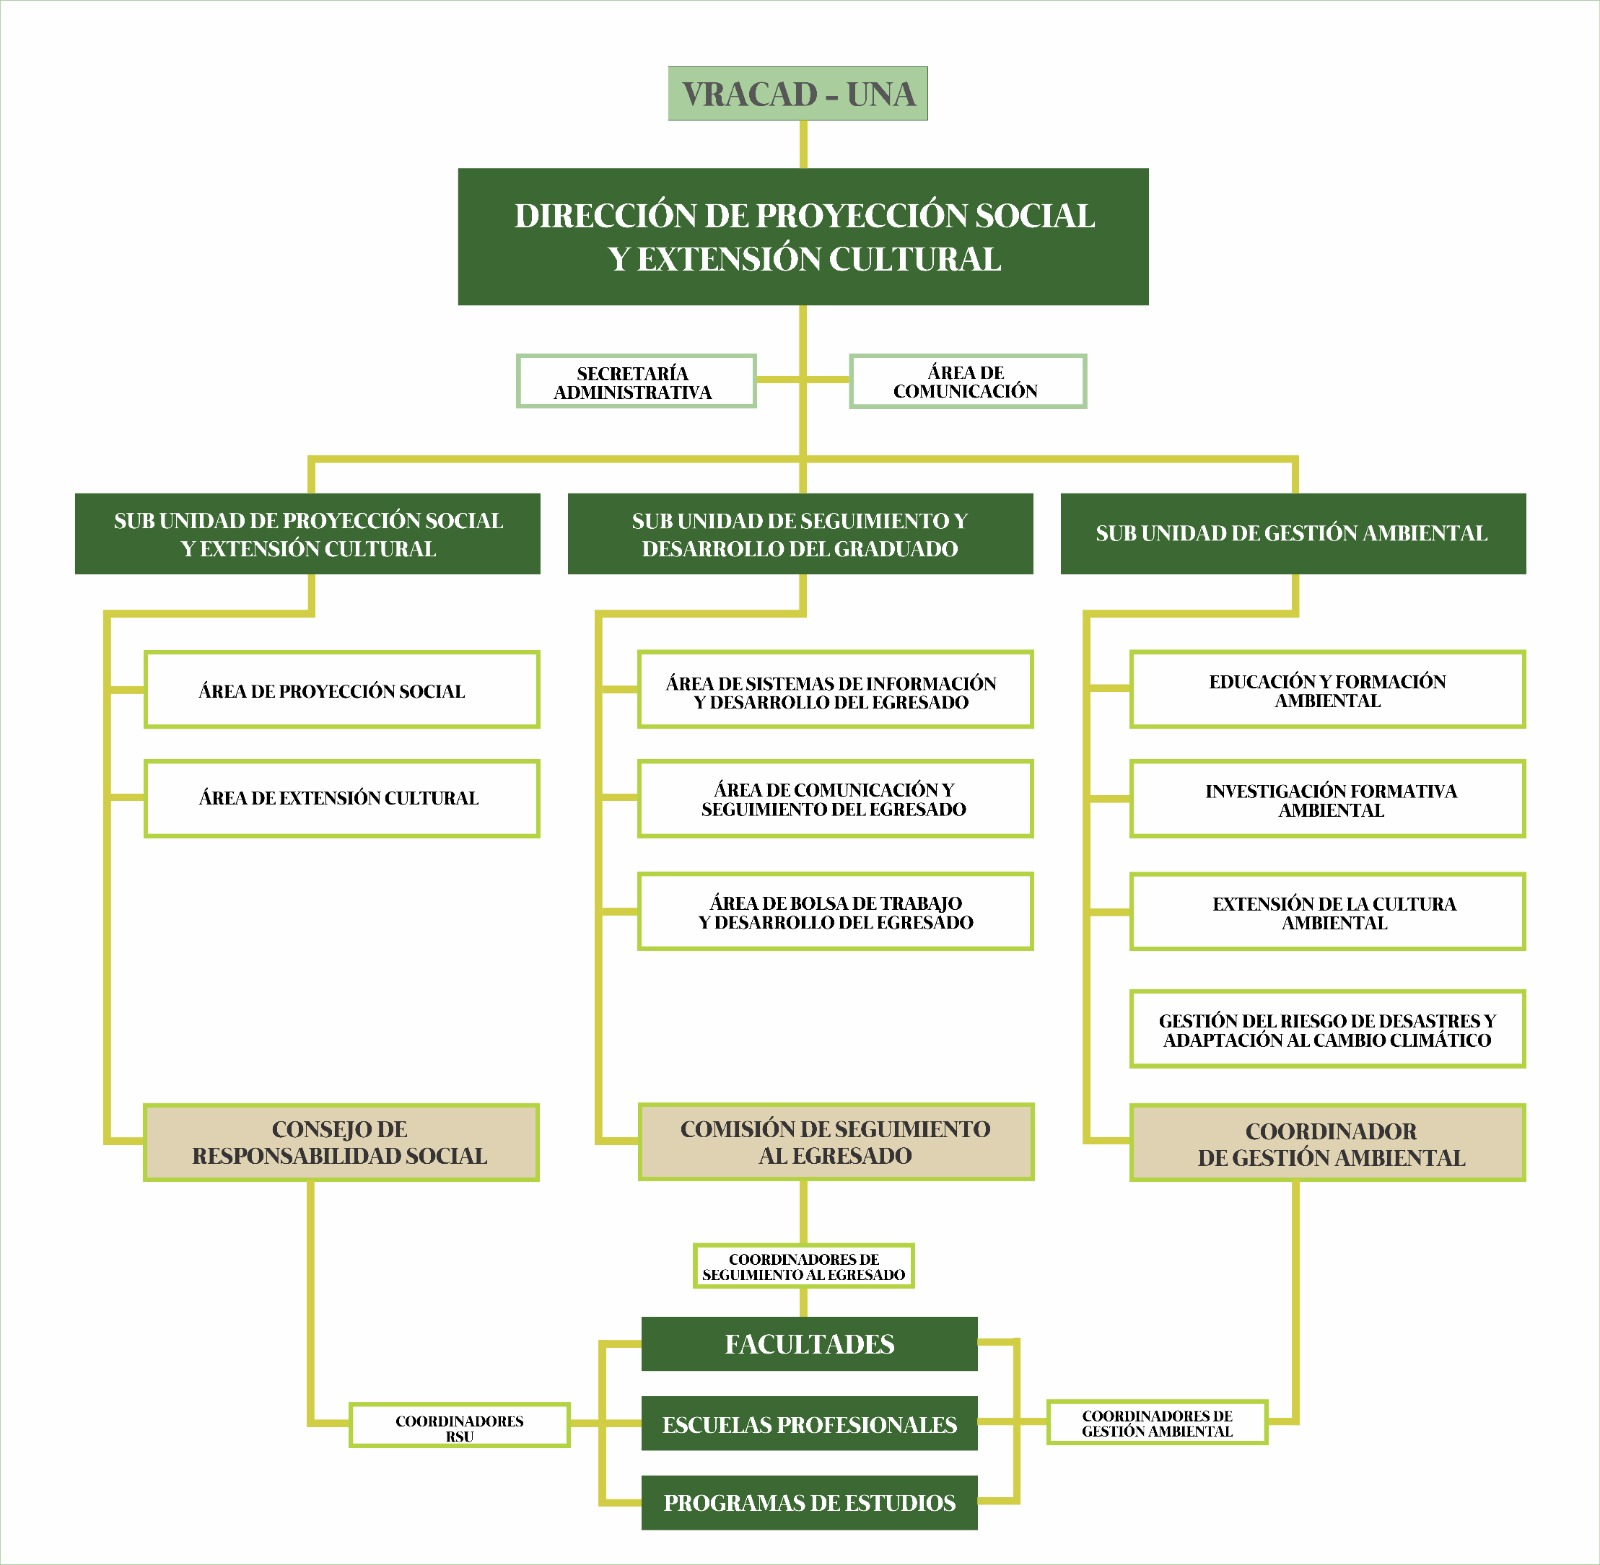
\includegraphics[width=0.8\textwidth]{assets/imagenes/estructura.jpeg} % Incluye la imagen y ajusta su ancho
    \label{fig:organigrama} % Etiqueta para referenciar
\end{figure}
\FloatBarrier


\section{Cumplimiento progresivo del plan de prácticas pre profesionales }

El puesto de Desarrollador de Software Frontend Junior en la Dirección de Proyección Social y Extensión Cultural desempeña un rol clave en el diseño, desarrollo y mantenimiento de soluciones tecnológicas que optimicen la operación de la institución. Este puesto no solo requiere habilidades técnicas en desarrollo frontend, sino también una comprensión profunda de los procesos institucionales para garantizar que las soluciones propuestas sean eficientes, de alta calidad, y alineadas con las necesidades específicas de la universidad.

El trabajo se desarrolló mediante un flujo iterativo e incremental: para cada funcionalidad se diseñó una propuesta, se presentó al supervisor o encargado de la oficina, se implementó y se ajustó a partir de la retroalimentación recibida. Este flujo es compatible con prácticas asociadas a Scrum y XP, sin afirmar la adopción completa de un marco formal.

\subsection*{Diagrama del Ciclo de Vida}
\begin{figure}[!htb] 
    \centering 
    \caption{Flujo iterativo de desarrollo}
    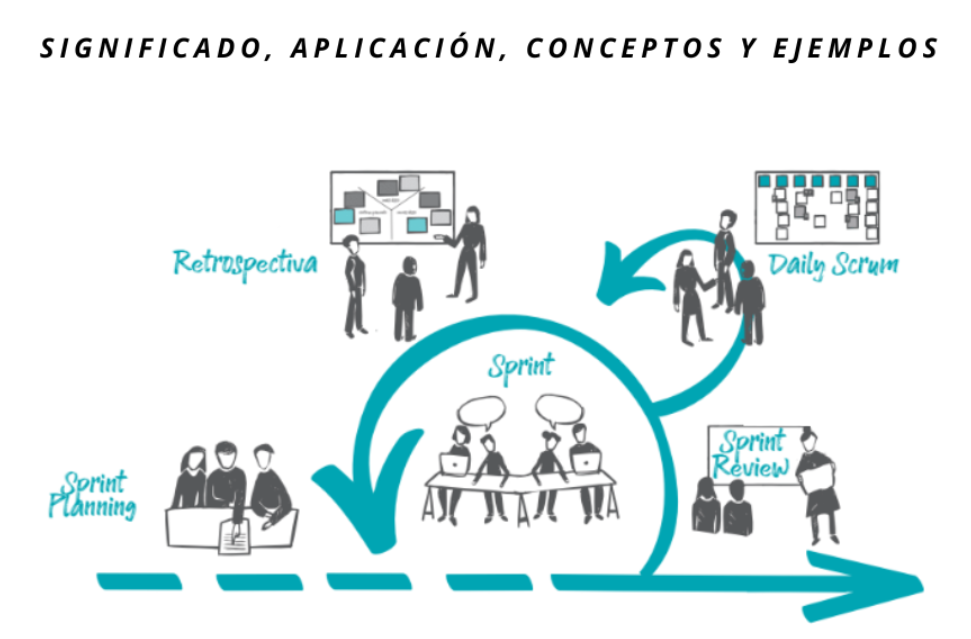
\includegraphics[width=0.9\textwidth]{assets/imagenes/SCRUM.png}
    \label{fig:scrum} 
\end{figure}
\FloatBarrier

\subsection{Actividad 1: Análisis de requerimientos del sistema}
\begin{table}[!htb]
    \centering
    \renewcommand{\arraystretch}{1.5} % Espaciado entre filas
    \begin{tabular}{|p{5cm}|p{10cm}|}
        \hline
        \textbf{Responsable de la actividad} & \PracticanteNombre \\ \hline
        \textbf{Objetivo de la actividad} & Mejorar y documentar los requerimientos funcionales de la primera versión y no funcionales del sistema de gestión de proyectos, para las tres subunidades de la Dirección de Proyección Social y Extensión Cultural. \\ \hline
        \textbf{Tareas realizadas} &
        \begin{itemize}
            \item Reuniones con el equipo de Proyección Social.
            \item Análisis de los procesos actuales de gestión.
            \item Documentación de los requerimientos en el sistema.
        \end{itemize} \\ \hline
        \textbf{Duración de la actividad} & 4 semanas \\ \hline
        \textbf{Fecha de inicio} & 15/04/25 \\ \hline
        \textbf{Fecha de culminación} & 15/05/25 \\ \hline
        \textbf{Materiales utilizados} &
        \begin{itemize}
            \item Laptop Huawei Matebook D16
            \item Visual Paradigm 16.2
        \end{itemize} \\ \hline
        %\textbf{Detalles de la actividad (Fotos)} & [Incluye fotos relevantes aquí si las tienes] \\ \hline
        \textbf{Resultados alcanzados} & Documento de especificaciones de requerimientos finalizado. \\ \hline
        \textbf{Porcentaje de avance} & 100\% \\ \hline
    \end{tabular}
    \caption{Resumen de la Actividad 1}
    \label{tab:actividad1}
\end{table}
\FloatBarrier

\begin{table}[!htb]
    \centering
    \renewcommand{\arraystretch}{1.5}

    \begin{tabularx}{\linewidth}{|p{0.30\linewidth}|Y|}
        \hline

        \textbf{Responsable de la actividad}
        & \PracticanteNombre \\ \hline

        \textbf{Objetivo de la actividad}
        & Mejorar y documentar los requerimientos funcionales de la primera versión y los requerimientos no funcionales del sistema de gestión de proyectos para las tres subunidades de la Dirección de Proyección Social y Extensión Cultural. \\ \hline

        \textbf{Tareas realizadas}
        &
        \begin{itemize}[nosep, leftmargin=*]
            \item Reuniones con el equipo de Proyección Social.
            \item Análisis de los procesos actuales de gestión.
            \item Documentación de los requerimientos en el sistema.
        \end{itemize}
        \\ \hline

        \textbf{Duración de la actividad}
        & 4 semanas \\ \hline

        \textbf{Fecha de inicio}
        & 15/04/25 \\ \hline

        \textbf{Fecha de culminación}
        & 15/05/25 \\ \hline

        \textbf{Materiales utilizados}
        &
        \begin{itemize}[nosep, leftmargin=*]
            \item Laptop Huawei MateBook D16.
            \item Visual Paradigm 16.2.
        \end{itemize}
        \\ \hline

        \textbf{Resultados alcanzados}
        & Documento de especificaciones de requerimientos finalizado. \\ \hline

        \textbf{Porcentaje de avance}
        & 100\% \\ \hline

    \end{tabularx}

    \caption{Resumen de la Actividad 1}
    \label{tab:actividad1_1}
\end{table}

\FloatBarrier

\subsubsection{Proceso de Recolección de Requerimientos}
En la fase de requerimientos, se realizó una entrevista estructurada con los usuarios finales y otras partes interesadas clave, incluyendo al personal de la Dirección de Proyección Social. Este paso fue fundamental para garantizar que el software se desarrolle alineado con las 
expectativas del cliente. 
Durante la entrevista y reunión evidenciada (ver Figura~\ref{fig:reunion}), se identificaron los siguientes requerimientos funcionales y no funcionales del sistema de gestión de proyectos:


\subsubsection{Requerimientos identificados}
\begin{table}[!htb]
    \centering  
        \caption{Lista de requerimientos funcionales}
    \begin{tabular}{p{6cm} p{6cm} }
        \toprule
        \textbf{Requerimiento funcional}  &   \textbf{Nombre del requerimiento}   \\
        \midrule
        RF-01   &   Gestionar roles \\
        RF-02   &   Gestionar permisos  \\
        RF-03   &   Gestionar usuarios  \\
        RF-04   &   Gestionar sub unidad    \\
        RF-05   &   Gestionar proyectos \\
        RF-06   &   Listar Proyectos    \\
        RF-07   &   Registrar voluntario    \\
        RF-08   &   Notificaciones  \\
        RF-09   &   Configuración de página \\
        RF-10   &   Gráficos estadísticos   \\
        \bottomrule
    \end{tabular}
\end{table}

\begin{table}[!htb]
    \centering  
        \caption{Lista de requerimientos no funcionales}
    \begin{tabular}{p{6cm} p{6cm} }
        \toprule
        \textbf{Requerimiento no funcional}  &   \textbf{Nombre del requerimiento}   \\
        \midrule
        RNF-01   &   Nivel de usuario \\
        RNF-02   &   Interfaz Intuitiva  \\
        RNF-03   &   Rapidez de carga  \\
        \bottomrule
    \end{tabular}
\end{table}
\begin{figure}[!htb] 
    \centering 
    \caption{Diagrama de casos de uso} 
    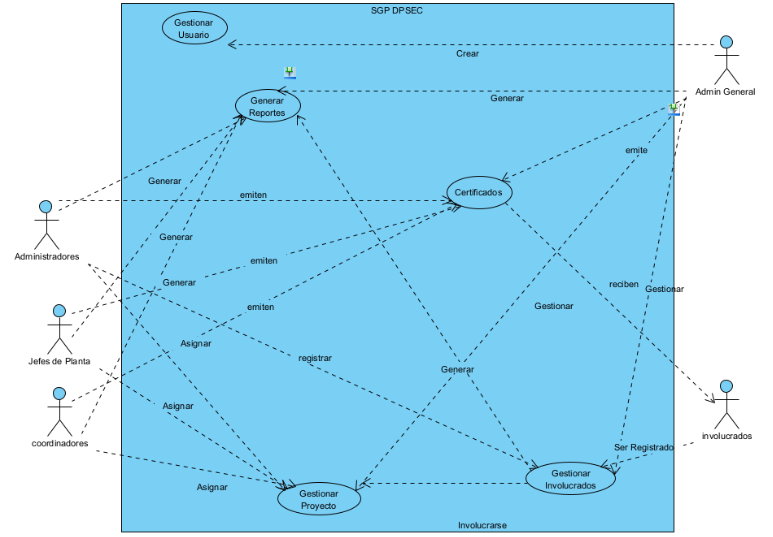
\includegraphics[width=0.8\textwidth]{assets/imagenes/casos_uso.png}
    \label{fig:casos_uso} 
\end{figure}
\FloatBarrier

\newpage
\subsubsection{Requerimiento funcionales}

\begin{table}[!htb]
    \centering
    \caption{Plantilla de los requerimientos}
    \begin{tabular}{|p{3cm}|p{10cm}|}
    \hline
    \textbf{Identificador} & \textit{ID único que identifica el requisito funcional.} \\ \hline
    \textbf{Nombre} & \textit{Nombre descriptivo del requisito funcional.} \\ \hline
    \textbf{Rol} & \textit{Rol del usuario relacionado con este requisito.} \\ \hline
    \textbf{Funcionalidad} & \textit{Descripción detallada de la funcionalidad que se espera.} \\ \hline
    \textbf{Resultado} & \textit{Resultado esperado después de ejecutar la funcionalidad.} \\ \hline
    \textbf{Precondición} & \textit{Condiciones que deben cumplirse antes de ejecutar este requisito.} \\ \hline
    \textbf{Postcondición} & \textit{Estado esperado del sistema después de ejecutar el requisito.} \\ \hline
    \textbf{Flujo Normal de Eventos} & \textit{Secuencia típica de pasos para cumplir el requisito.} \\ \hline
    \textbf{Flujo Alternativo y Excepciones} & \textit{Descripciones de posibles desviaciones o errores en el flujo.} \\ \hline
    \end{tabular}
    \label{tabla:req-funcionales}
\end{table}
\FloatBarrier


\begin{table}[htb!]
    \centering
    \caption{Requisito Funcional RF-01}
\begin{tabular}{|p{4cm}|p{12cm}|}
\hline
\textbf{Campo} & \textbf{Descripcion} \\ \hline
\textbf{Identificador} & RF-01 \\ \hline
\textbf{Nombre} & Gestionar Roles \\ \hline
\textbf{Rol} & Administrador \\ \hline
\textbf{Funcionalidad} & Crear, editar y eliminar roles en el sistema. \\ \hline
\textbf{Resultado} & Permitir una asignacion clara de permisos a diferentes usuarios segun sus responsabilidades. \\ \hline
\textbf{Precondicion} & El usuario debe estar autenticado como administrador. \\ \hline
\textbf{Postcondicion} & Los roles seran visibles y asignables a los usuarios. \\ \hline
\textbf{Flujo Normal de Eventos} & 
\begin{enumerate}
    \item El administrador accede al modulo de gestion de roles. 
    \item Selecciona la opcion de crear, editar o eliminar un rol. 
    \item Ingresa o modifica los detalles del rol (nombre, descripcion, permisos).
    \item Confirma la accion y guarda los cambios.  
\end{enumerate}
\\ \hline 
\textbf{Flujo Alternativo y Excepciones} & 
\begin{itemize}
    \item Si faltan datos obligatorios, se muestra un mensaje de error indicando los campos requeridos. 
    \item Si intenta eliminar un rol asignado, se muestra un aviso para reasignar usuarios. 
    
\end{itemize}
\\ \hline
\end{tabular}
\end{table}
\FloatBarrier

\begin{table}[htb!]
\centering
\caption{Requisito Funcional RF-02}
\begin{tabular}{|p{3cm}|p{12cm}|}
\hline
\textbf{Campo} & \textbf{Descripcion} \\ \hline
\textbf{Identificador} & RF-02 \\ \hline
\textbf{Nombre} & Gestionar Permisos \\ \hline
\textbf{Rol} & Administrador \\ \hline
\textbf{Funcionalidad} & Definir, asignar y modificar permisos en el sistema. \\ \hline
\textbf{Resultado} & Garantizar que cada rol tenga los permisos adecuados para las funciones asignadas. \\ \hline
\textbf{Precondicion} & - El usuario debe estar autenticado como administrador. \\ \hline
\textbf{Postcondicion} & Los permisos estaran asociados correctamente a los roles. \\ \hline
\textbf{Flujo Normal de Eventos} & 
\begin{enumerate}
    \item El administrador accede al modulo de gestión de permisos. 
    \item Selecciona la opcion de crear, editar o eliminar un permiso. 
    \item Ingresa o modifica los detalles del permiso (nombre, descripcion, nivel de acceso). 
    \item Guarda los cambios.
    
\end{enumerate}
\\ \hline
\textbf{Flujo Alternativo y Excepciones} & 
- Si intenta eliminar un permiso asignado, el sistema solicita reasignar o deshabilitar el permiso. \\ \hline
\end{tabular}
\end{table}
\FloatBarrier

\begin{table}[htb!]
    \centering
    \caption{Requisito Funcional RF-03}
\begin{tabular}{|p{3cm}|p{12cm}|}
\hline
\textbf{Campo} & \textbf{Descripcion} \\ \hline
\textbf{Identificador} & RF-03 \\ \hline
\textbf{Nombre} & Gestionar Usuarios \\ \hline
\textbf{Rol} & Administrador \\ \hline
\textbf{Funcionalidad} & Registrar, actualizar y desactivar usuarios en el sistema. \\ \hline
\textbf{Resultado} & Mantener un control centralizado sobre las cuentas activas en el sistema. \\ \hline
\textbf{Precondicion} & El usuario debe estar autenticado como administrador. \\ \hline
\textbf{Postcondicion} & Los usuarios registrados tendran acceso segun su rol. \\ \hline
\textbf{Flujo Normal de Eventos} & 
\begin{enumerate}
    \item El administrador accede al modulo de gestion de usuarios. 
    \item Selecciona la opcion de registrar, editar o desactivar un usuario. 
    \item Ingresa o modifica los datos del usuario (nombre, correo, rol). 
    \item Confirma los cambios.
    
\end{enumerate}
\\ \hline
\textbf{Flujo Alternativo y Excepciones} & 
- Si el correo ya esta registrado, se muestra un mensaje de error. \\ \hline
\end{tabular}
\end{table}
\FloatBarrier

\begin{table}[htb!]
\centering
\caption{Requisito Funcional RF-04}
\begin{tabular}{|p{3cm}|p{12cm}|}
\hline
\textbf{Campo} & \textbf{Descripcion} \\ \hline
\textbf{Identificador} & RF-04 \\ \hline
\textbf{Nombre} & Gestionar Subunidades \\ \hline
\textbf{Rol} & Administrador \\ \hline
\textbf{Funcionalidad} & Organizar y administrar subunidades dentro de una unidad principal. \\ \hline
\textbf{Resultado} & Facilitar la organizacion jerarquica del sistema. \\ \hline
\textbf{Precondicion} & El usuario debe estar autenticado como administrador. \\ \hline
\textbf{Postcondicion} & Las subunidades estaran vinculadas a la unidad principal correspondiente. \\ \hline
\textbf{Flujo Normal de Eventos} & 
\begin{enumerate}
    \item El administrador accede al modulo de subunidades. 
    \item Selecciona la opcion de registrar, editar o eliminar una subunidad. 
    \item Ingresa o modifica los datos de la subunidad (nombre, descripcion). 
    \item Guarda los cambios. 
    
\end{enumerate}
\\ \hline
\textbf{Flujo Alternativo y Excepciones} & 
- Si la subunidad tiene dependencias activas, no puede eliminarse hasta resolverlas. \\ \hline
\end{tabular}
\end{table}
\FloatBarrier

\begin{table}[htb!]
\centering
\caption{Requisito Funcional RF-05}
\begin{tabular}{|p{3cm}|p{12cm}|}
\hline
\textbf{Campo} & \textbf{Descripcion} \\ \hline
\textbf{Identificador} & RF-05 \\ \hline
\textbf{Nombre} & Gestionar Proyectos \\ \hline
\textbf{Rol} & Administrador \\ \hline
\textbf{Funcionalidad} & Registrar, actualizar, eliminar y listar proyectos. \\ \hline
\textbf{Resultado} & Organizar y administrar proyectos en curso y completados. \\ \hline
\textbf{Precondicion} & El usuario debe estar autenticado como administrador. \\ \hline
\textbf{Postcondicion} & Los proyectos estaran disponibles para asignar recursos y seguimiento. \\ \hline
\textbf{Flujo Normal de Eventos} & 
\begin{enumerate}
    \item El administrador accede al modulo de proyectos. 
    \item Selecciona la opcion de registrar, editar o eliminar un proyecto. 
    \item Ingresa o modifica los datos del proyecto (nombre, descripcion, responsables). 
    \item Guarda los cambios.
    
\end{enumerate}
\\ \hline
\textbf{Flujo Alternativo y Excepciones} & 
- Si no hay datos disponibles para el proyecto, se muestra un mensaje indicando que no hay informacion suficiente. \\ \hline
\end{tabular}
\end{table}
\FloatBarrier

\begin{table}[htb!]
\centering
\caption{Requisito Funcional RF-06}
\begin{tabular}{|p{3cm}|p{12cm}|}
\hline
\textbf{Campo} & \textbf{Descripcion} \\ \hline
\textbf{Identificador} & RF-06 \\ \hline
\textbf{Nombre} & Listar Proyectos \\ \hline
\textbf{Rol} & Administrador, Usuario General \\ \hline
\textbf{Funcionalidad} & Mostrar una lista de todos los proyectos registrados, con opcion de filtrado y busqueda. \\ \hline
\textbf{Resultado} & Facilitar el acceso y visualizacion de proyectos para su monitoreo y consulta. \\ \hline
\textbf{Precondicion} & El usuario debe estar autenticado en el sistema. \\ \hline
\textbf{Postcondicion} & Se genera una lista visible de proyectos con detalles basicos como nombre, estado y responsables. \\ \hline
\textbf{Flujo Normal de Eventos} & 
\begin{enumerate}
    \item El usuario accede al modulo de proyectos. 
    \item Selecciona la opcion de listar proyectos. 
    \item Se despliega una lista con filtros de busqueda (por estado, responsables, fecha, etc.). 
    \item El usuario visualiza o selecciona un proyecto para mas detalles. 
    
\end{enumerate}
\\ \hline
\textbf{Flujo Alternativo y Excepciones} & 
- Si no hay proyectos registrados, se muestra un mensaje indicando que no hay datos disponibles. \\ \hline
\end{tabular}
\end{table}
\FloatBarrier

\begin{table}[htb!]
\centering
\caption{Requisito Funcional RF-07}
\begin{tabular}{|p{3cm}|p{12cm}|}
\hline
\textbf{Campo} & \textbf{Descripcion} \\ \hline
\textbf{Identificador} & RF-07 \\ \hline
\textbf{Nombre} & Registrar Voluntario \\ \hline
\textbf{Rol} & Usuario \\ \hline
\textbf{Funcionalidad} & Permitir el registro de voluntarios con sus datos personales y habilidades. \\ \hline
\textbf{Resultado} & Incorporar voluntarios al sistema para asignarlos a proyectos especificos. \\ \hline
\textbf{Precondicion} & El usuario debe estar autenticado como administrador. \\ \hline
\textbf{Postcondicion} & El voluntario queda registrado y disponible para asignacion en proyectos. \\ \hline
\textbf{Flujo Normal de Eventos} & 
\begin{enumerate}
    \item El administrador accede al modulo de registro de voluntarios. 
    \item Completa el formulario con los datos del voluntario (nombre, contacto, habilidades). 
    \item Confirma el registro y guarda la informacion. 
    
\end{enumerate}
\\ \hline
\textbf{Flujo Alternativo y Excepciones} & 
- Si algun dato obligatorio falta, se muestra un mensaje indicando los campos requeridos. \\ \hline
\end{tabular}
\end{table}
\FloatBarrier

\begin{table}[htb!]
\centering
\caption{Requisito Funcional RF-08}
\begin{tabular}{|p{3cm}|p{12cm}|}
\hline
\textbf{Campo} & \textbf{Descripcion} \\ \hline
\textbf{Identificador} & RF-08 \\ \hline
\textbf{Nombre} & Notificaciones \\ \hline
\textbf{Rol} & Administrador, Usuario General \\ \hline
\textbf{Funcionalidad} & Enviar notificaciones relacionadas con proyectos, actividades o eventos importantes. \\ \hline
\textbf{Resultado} & Mantener a los usuarios informados sobre actualizaciones relevantes en tiempo real. \\ \hline
\textbf{Precondicion} & El usuario debe estar autenticado en el sistema. \\ \hline
\textbf{Postcondicion} & Los usuarios reciben las notificaciones configuradas en sus cuentas. \\ \hline
\textbf{Flujo Normal de Eventos} & 
\begin{enumerate}
    \item El usuario accede al modulo de notificaciones. 
    \item Configura o visualiza las notificaciones enviadas. 
    \item El sistema entrega la notificacion segun las preferencias configuradas (correo, SMS, app). 
    
\end{enumerate}
\\ \hline
\textbf{Flujo Alternativo y Excepciones} & 
- Si la configuracion de notificaciones falla, el sistema muestra un error e intenta nuevamente. \\ \hline
\end{tabular}
\end{table}
\FloatBarrier

\begin{table}[htb!]
\centering
\caption{Requisito Funcional RF-09}
\begin{tabular}{|p{3cm}|p{12cm}|}
\hline
\textbf{Campo} & \textbf{Descripcion} \\ \hline
\textbf{Identificador} & RF-09 \\ \hline
\textbf{Nombre} & Configuracion de Pagina \\ \hline
\textbf{Rol} & Administrador \\ \hline
\textbf{Funcionalidad} & Personalizar elementos basicos de la pagina, como logotipo, colores y textos predeterminados. \\ \hline
\textbf{Resultado} & Adaptar la interfaz del sistema a las necesidades de la organizacion. \\ \hline
\textbf{Precondicion} & El usuario debe estar autenticado como administrador. \\ \hline
\textbf{Postcondicion} & Los cambios se reflejan inmediatamente en la interfaz del sistema. \\ \hline
\textbf{Flujo Normal de Eventos} & 
\begin{enumerate}
    \item El administrador accede al modulo de configuracion. 
    \item Selecciona la opcion a personalizar (logotipo, colores, etc.). 
    \item Realiza los cambios deseados y los guarda. 
    
\end{enumerate}
\\ \hline
\textbf{Flujo Alternativo y Excepciones} & 
- Si el archivo subido (como logotipo) no cumple con los requisitos, el sistema muestra un error indicando el problema. \\ \hline
\end{tabular}
\end{table}
\FloatBarrier

\begin{table}[htb!]
\centering
\caption{Requisito Funcional RF-10}
\begin{tabular}{|p{3cm}|p{12cm}|}
\hline
\textbf{Campo} & \textbf{Descripcion} \\ \hline
\textbf{Identificador} & RF-10 \\ \hline
\textbf{Nombre} & Graficos Estadisticos \\ \hline
\textbf{Rol} & Administrador, Usuario General \\ \hline
\textbf{Funcionalidad} & Generar y visualizar graficos basados en los datos del sistema, como estadisticas de proyectos y usuarios. \\ \hline
\textbf{Resultado} & Proveer una vision clara y visual de los datos relevantes para la toma de decisiones. \\ \hline
\textbf{Precondicion} & El usuario debe estar autenticado en el sistema. \\ \hline
\textbf{Postcondicion} & Los graficos estaran disponibles y actualizados segun los datos mas recientes. \\ \hline
\textbf{Flujo Normal de Eventos} & 
\begin{enumerate}
    \item El usuario accede al modulo de estadisticas. 
    \item Selecciona los datos o metricas a visualizar. 
    \item El sistema genera los graficos correspondientes. 
    \item El usuario consulta o exporta los graficos si es necesario.
\end{enumerate}
\\ \hline
\textbf{Flujo Alternativo y Excepciones} & 
- Si no hay datos disponibles para generar graficos, el sistema muestra muestra un mensaje indicando la falta de datos. \\ \hline
\end{tabular}
\end{table}
\FloatBarrier

\subsubsection{Requerimientos no funcionales}

\begin{table}[htb!]
    \centering
    \caption{Requisito Funcional RNF-01}
    \begin{tabular}{|p{3cm}|p{12cm}|}
    \hline
    \textbf{Campo} & \textbf{Descripcion} \\ \hline
    \textbf{Identificador} & RNF-01 \\ \hline
    \textbf{Nombre} &  Nivel de Usuario \\ \hline
    \textbf{Descripción} &  El sistema debe ser accesible para usuarios con diferentes niveles de experiencia técnica, asegurando que tanto administradores como usuarios generales puedan interactuar de manera efectiva. \\ \hline
    \textbf{Resultado} &  Garantizar que el sistema sea útil para una variedad de usuarios sin requerir conocimientos técnicos avanzados. \\ \hline
    \textbf{Creiterios de aceptación} & 
    \begin{enumerate}
        \item El sistema incluye ayudas contextuales y tutoriales básicos.
        \item La interfaz está diseñada con un enfoque amigable y accesible para todos los roles.
        
    \end{enumerate}
    \\ \hline
    \textbf{Restricciones} & El diseño debe considerar las mejores prácticas de usabilidad. \\ \hline
    
\end{tabular}
\end{table}
\FloatBarrier

    \begin{table}[htb!]
        \centering
        \caption{Requisito Funcional RNF-02}
        \begin{tabular}{|p{3cm}|p{12cm}|}
        \hline
        \textbf{Campo} & \textbf{Descripcion} \\ \hline
        \textbf{Identificador} & RNF-02 \\ \hline
        \textbf{Nombre} & Interfaz Intuitiva \\ \hline
        \textbf{Descripción} & La interfaz gráfica del sistema debe ser clara, ordenada y permitir a los usuarios realizar tareas con la menor cantidad de clics posible. \\ \hline
        \textbf{Resultado} & Facilitar el uso del sistema y minimizar errores de operación por parte de los usuarios. \\ \hline
        \textbf{Creiterios de aceptación} & 
        \begin{enumerate}
            \item La navegación debe seguir estándares comunes (menú superior, botones claros).
            \item Elementos interactivos deben estar debidamente etiquetados y ser fácilmente identificables.
            
        \end{enumerate}
        \\ \hline
        \textbf{Restricciones} & Debe implementarse un diseño responsive para dispositivos móviles y de escritorio. \\ \hline
        
    \end{tabular}
    \end{table}
    \FloatBarrier


    \begin{table}[htb!]
        \centering
        \caption{Requisito Funcional RNF-03}
        \begin{tabular}{|p{3cm}|p{12cm}|}
        \hline
        \textbf{Campo} & \textbf{Descripcion} \\ \hline
        \textbf{Identificador} & RNF-03 \\ \hline
        \textbf{Nombre} & Rapidez de Carga \\ \hline
        \textbf{Descripción} & El tiempo de carga del sistema no debe exceder los 2 segundos para la mayoría de las interacciones estándar en condiciones normales. \\ \hline
        \textbf{Resultado} & Mejorar la experiencia del usuario y la eficiencia en la interacción con el sistema. \\ \hline
        \textbf{Creiterios de aceptación} & 
        \begin{enumerate}
            \item Las páginas principales del sistema deben cargarse en menos de 2 segundos con conexión a internet estándar (10 Mbps).
            \item Los tiempos de respuesta de las consultas a la base de datos no deben exceder 1 segundo.    
             
        \end{enumerate}

        \\ \hline
        \textbf{Restricciones} & Se debe implementar caching y optimización de consultas para garantizar el rendimiento. \\ \hline
        
    \end{tabular}
    \end{table}
    \FloatBarrier

\subsubsection{Diagrama de clases}
Los diagramas de clases representan las entidades principales del sistema (clases) y sus atributos (propiedades) y métodos (comportamientos).
Ayudan a visualizar cómo están organizadas las partes del software antes de escribir código.
\begin{figure}[!htb]
    \centering
    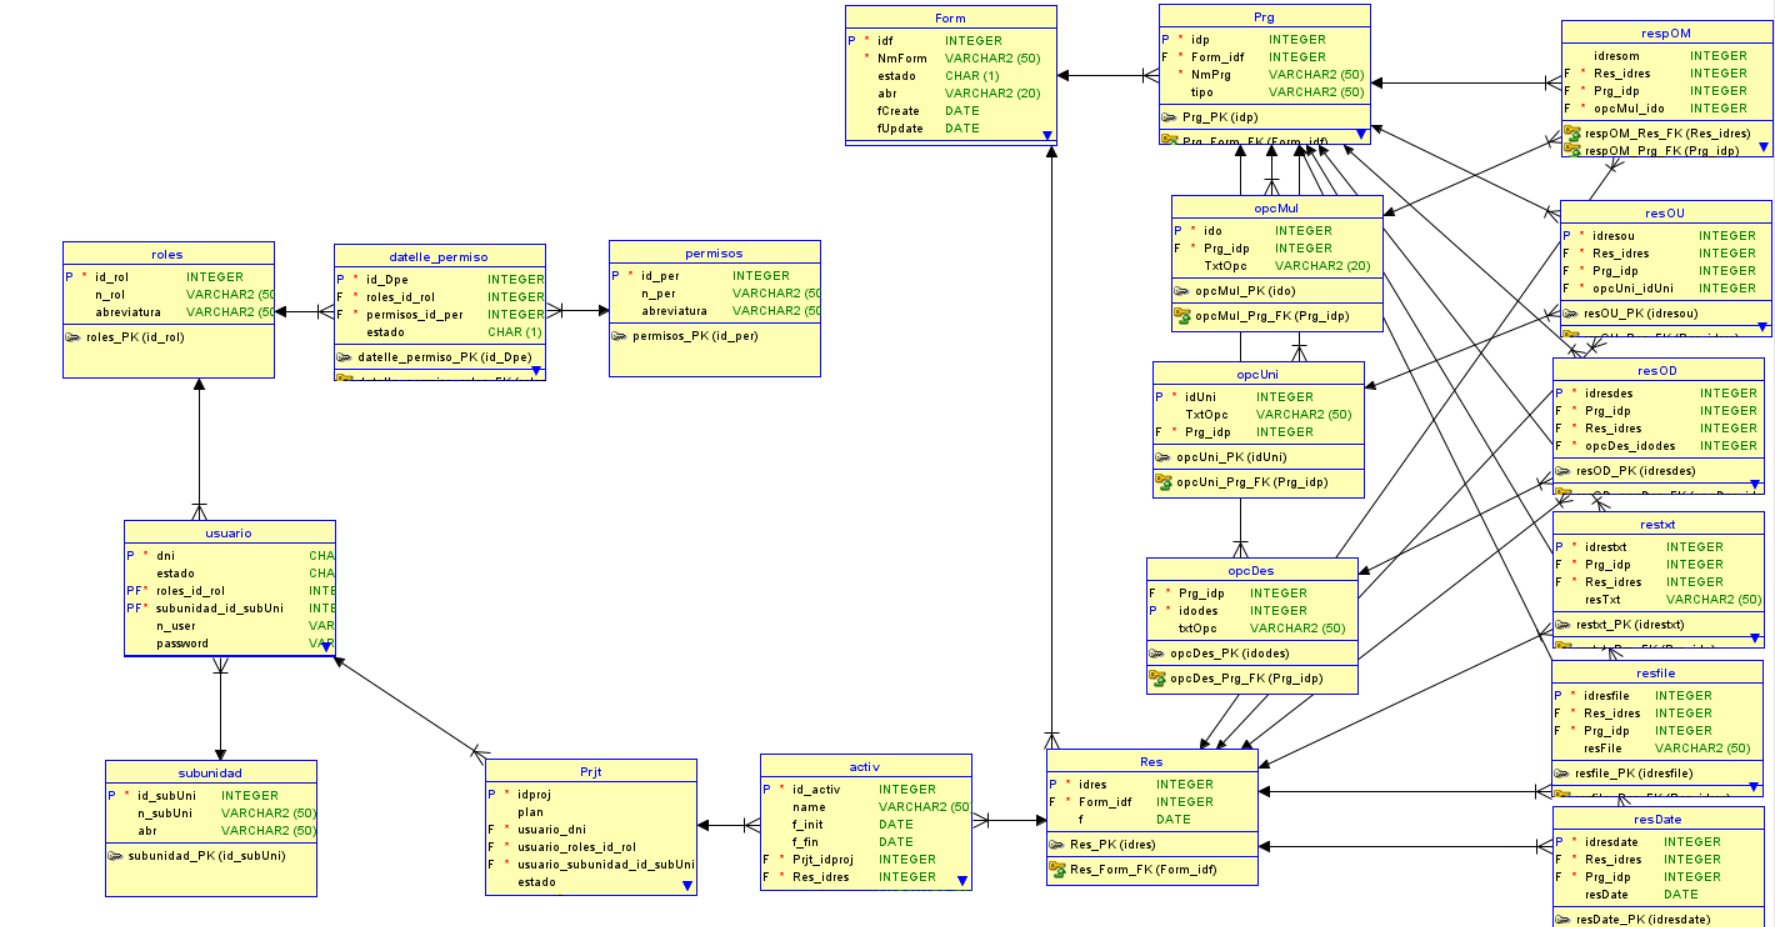
\includegraphics[width=0.8\textwidth]{assets/imagenes/clases.png}
    \caption{Diagrama de Clases del Sistema.}
    \label{fig:clases}
\end{figure}
\FloatBarrier





\subsection{Actividad 2: Diseño}
\begin{table}[!htb]
    \centering
    \caption{Resumen de la Actividad 2}
    \begin{tabular}{|p{5cm}|p{10cm}|}
        \hline
        \textbf{Responsable de la actividad} & \PracticanteNombre \\ \hline
        \textbf{Objetivo de la actividad} & Diseñar el sistema en relación con los requerimientos recogidos\\ \hline
        \textbf{Tareas realizadas} &
        \begin{itemize}
            \item Diseño de la interfaz por modulos.
        \end{itemize} \\ \hline
        \textbf{Duración de la actividad} & 2 semanas \\ \hline
        \textbf{Fecha de inicio} & 16/05/25 \\ \hline
        \textbf{Fecha de culminación} & 31/05/25 \\ \hline
        \textbf{Materiales utilizados} &
        \begin{itemize}
            \item Laptop Huawei Matebook D16
            \item Figma 16.2
        \end{itemize} \\ \hline
        %\textbf{Detalles de la actividad (Fotos)} & [Incluye fotos relevantes aquí si las tienes] \\ \hline
        \textbf{Resultados alcanzados} & Prototipo en un nivel de madurez muy alto como para que sea programado\\ \hline
        \textbf{Porcentaje de avance} & 90\% \\ \hline
    \end{tabular}
    \label{tab:actividad2}
\end{table}
\FloatBarrier

\subsubsection{Detalles de la actividad}
En esta actividad, se diseñó la interfaz del sistema en Figma, un software de diseño de interfaces de usuario. El diseño se realizó en base a los requerimientos recogidos en la actividad anterior, y se dividió en módulos para facilitar el desarrollo y la implementación. El prototipo final alcanzó un nivel de madurez muy alto, lo que permitirá una implementación ágil y eficiente en la siguiente fase del proyecto segun SCRUM.\\
\href{https://www.figma.com/proto/sV0jV2oSvDyUHLI0Pm1KzV/DPSEC?node-id=563-3455&t=SQIVi97HhkuWXdes-1&scaling=scale-down&content-scaling=fixed&page-id=0%3A1&starting-point-node-id=21%3A4&show-proto-sidebar=1}{Ver prototipo en Figma}

\begin{figure}[!htb] 
    \centering 
    \caption{Diseño de la interfaz de pagina principal publico} 
    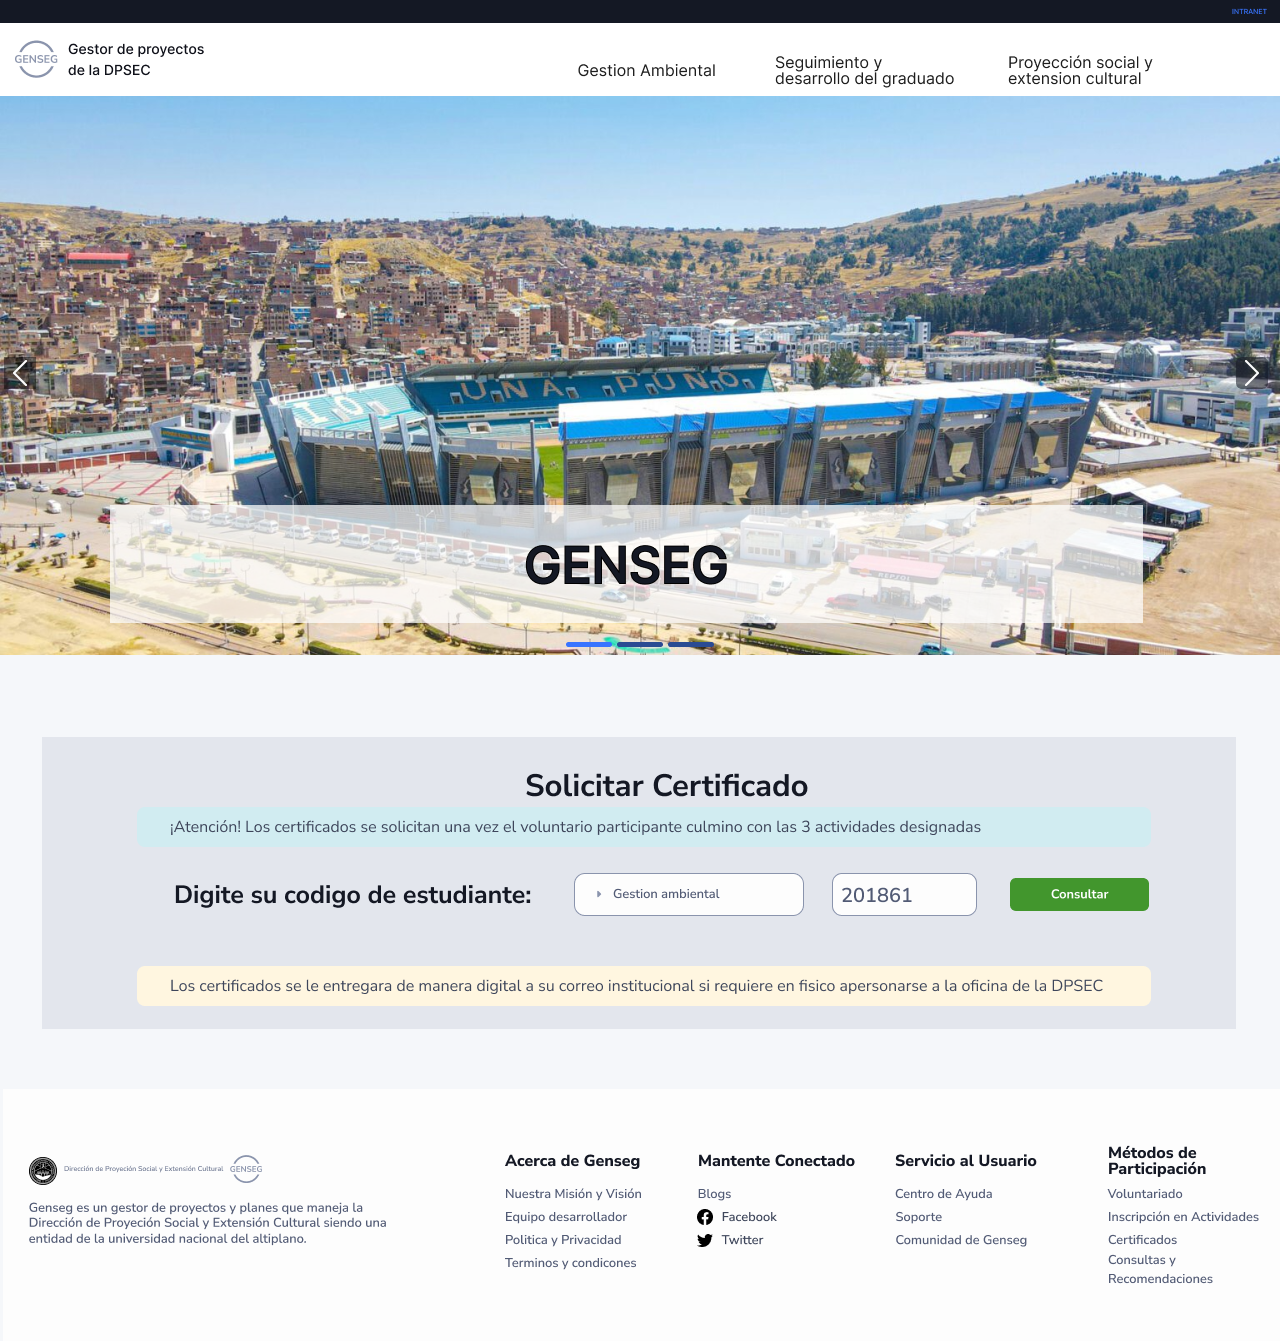
\includegraphics[width=0.8\textwidth]{assets/imagenes/paginaprincipal.png}
    \label{fig:paginaprincipal} 
\end{figure} 
\FloatBarrier

\begin{figure}[!htb] 
    \centering 
    \caption{Diseño de solicitud de certificados} 
    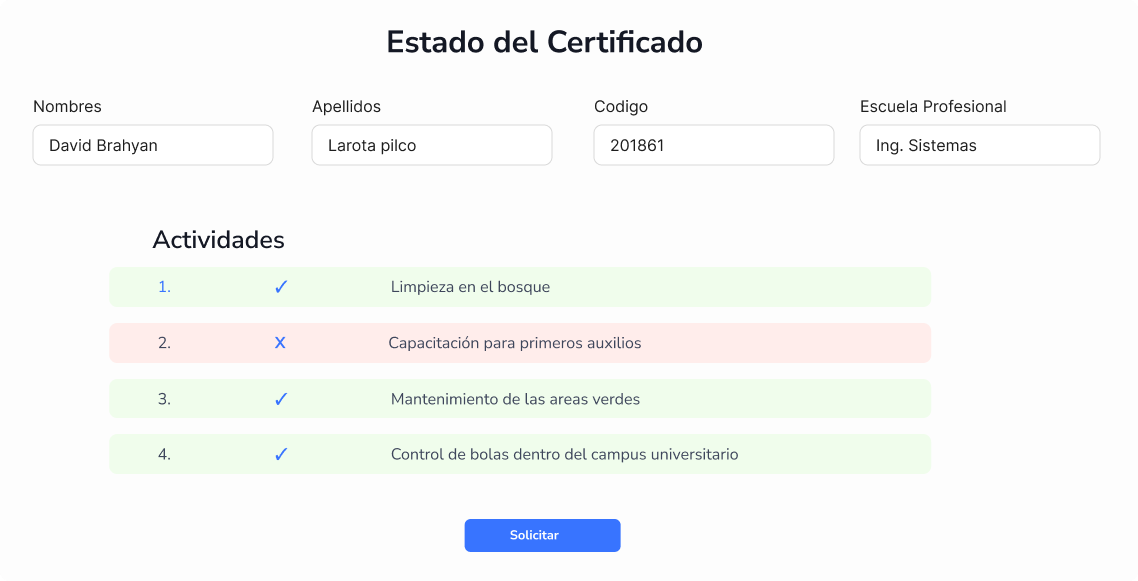
\includegraphics[width=0.8\textwidth]{assets/imagenes/certificado.png}
    \label{fig:certificado} 
\end{figure} 
\FloatBarrier

\begin{figure}[!htb] 
    \centering 
    \caption{Intranet - Login} 
    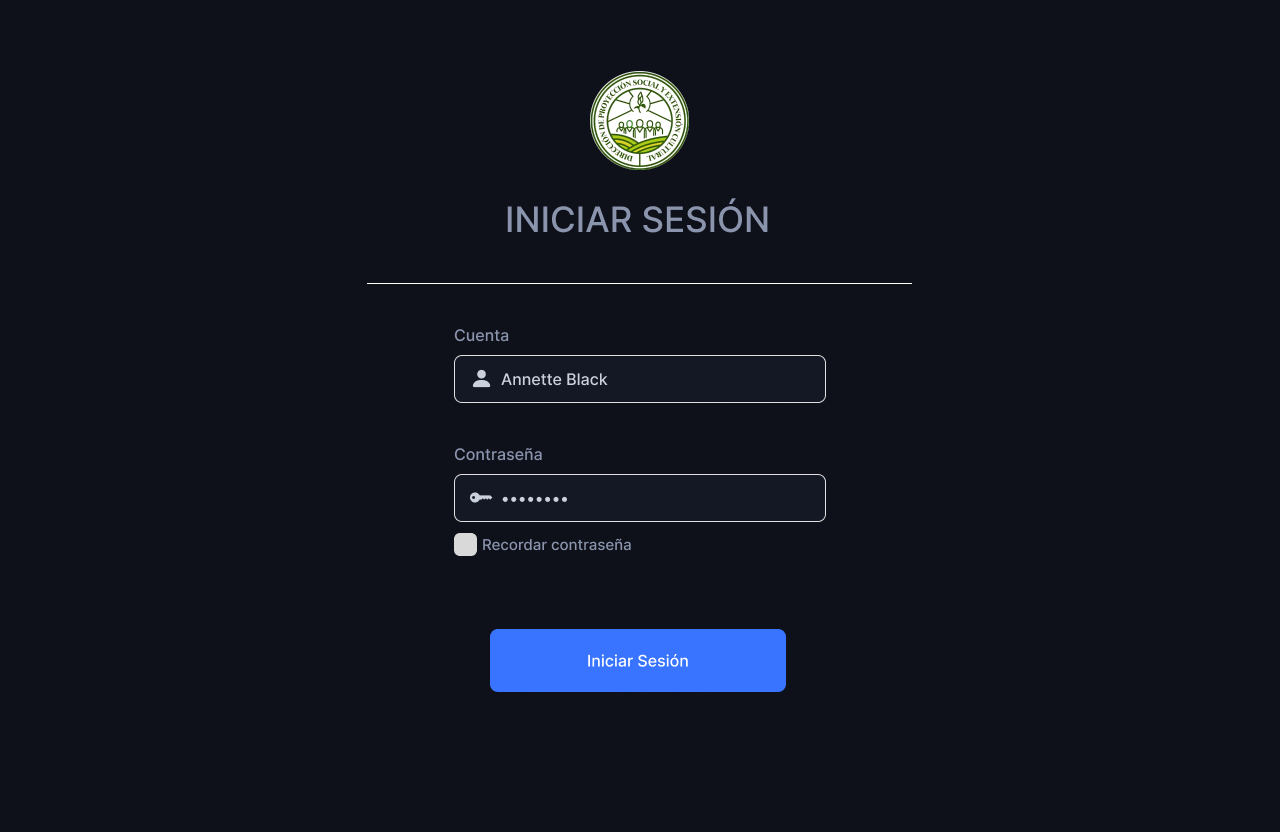
\includegraphics[width=0.8\textwidth]{assets/imagenes/intranet_login.png}
    \label{fig:intranet_login} 
\end{figure} 
\FloatBarrier

\begin{figure}[!htb] 
    \centering 
    \caption{Intranet - Escoger roles} 
    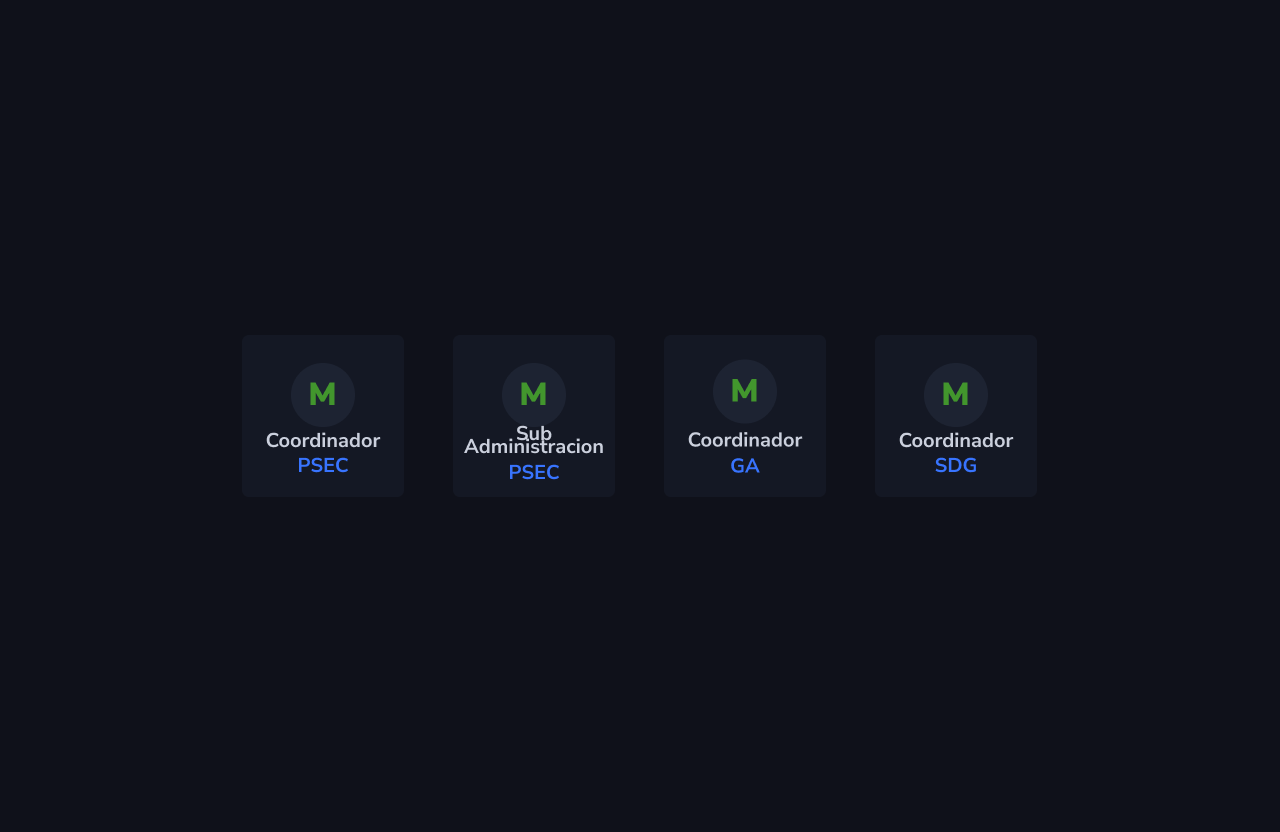
\includegraphics[width=0.8\textwidth]{assets/imagenes/roles.png}
    \label{fig:roles} 
\end{figure} 
\FloatBarrier

\begin{figure}[!htb] 
    \centering 
    \caption{Intranet - Pagina principal} 
    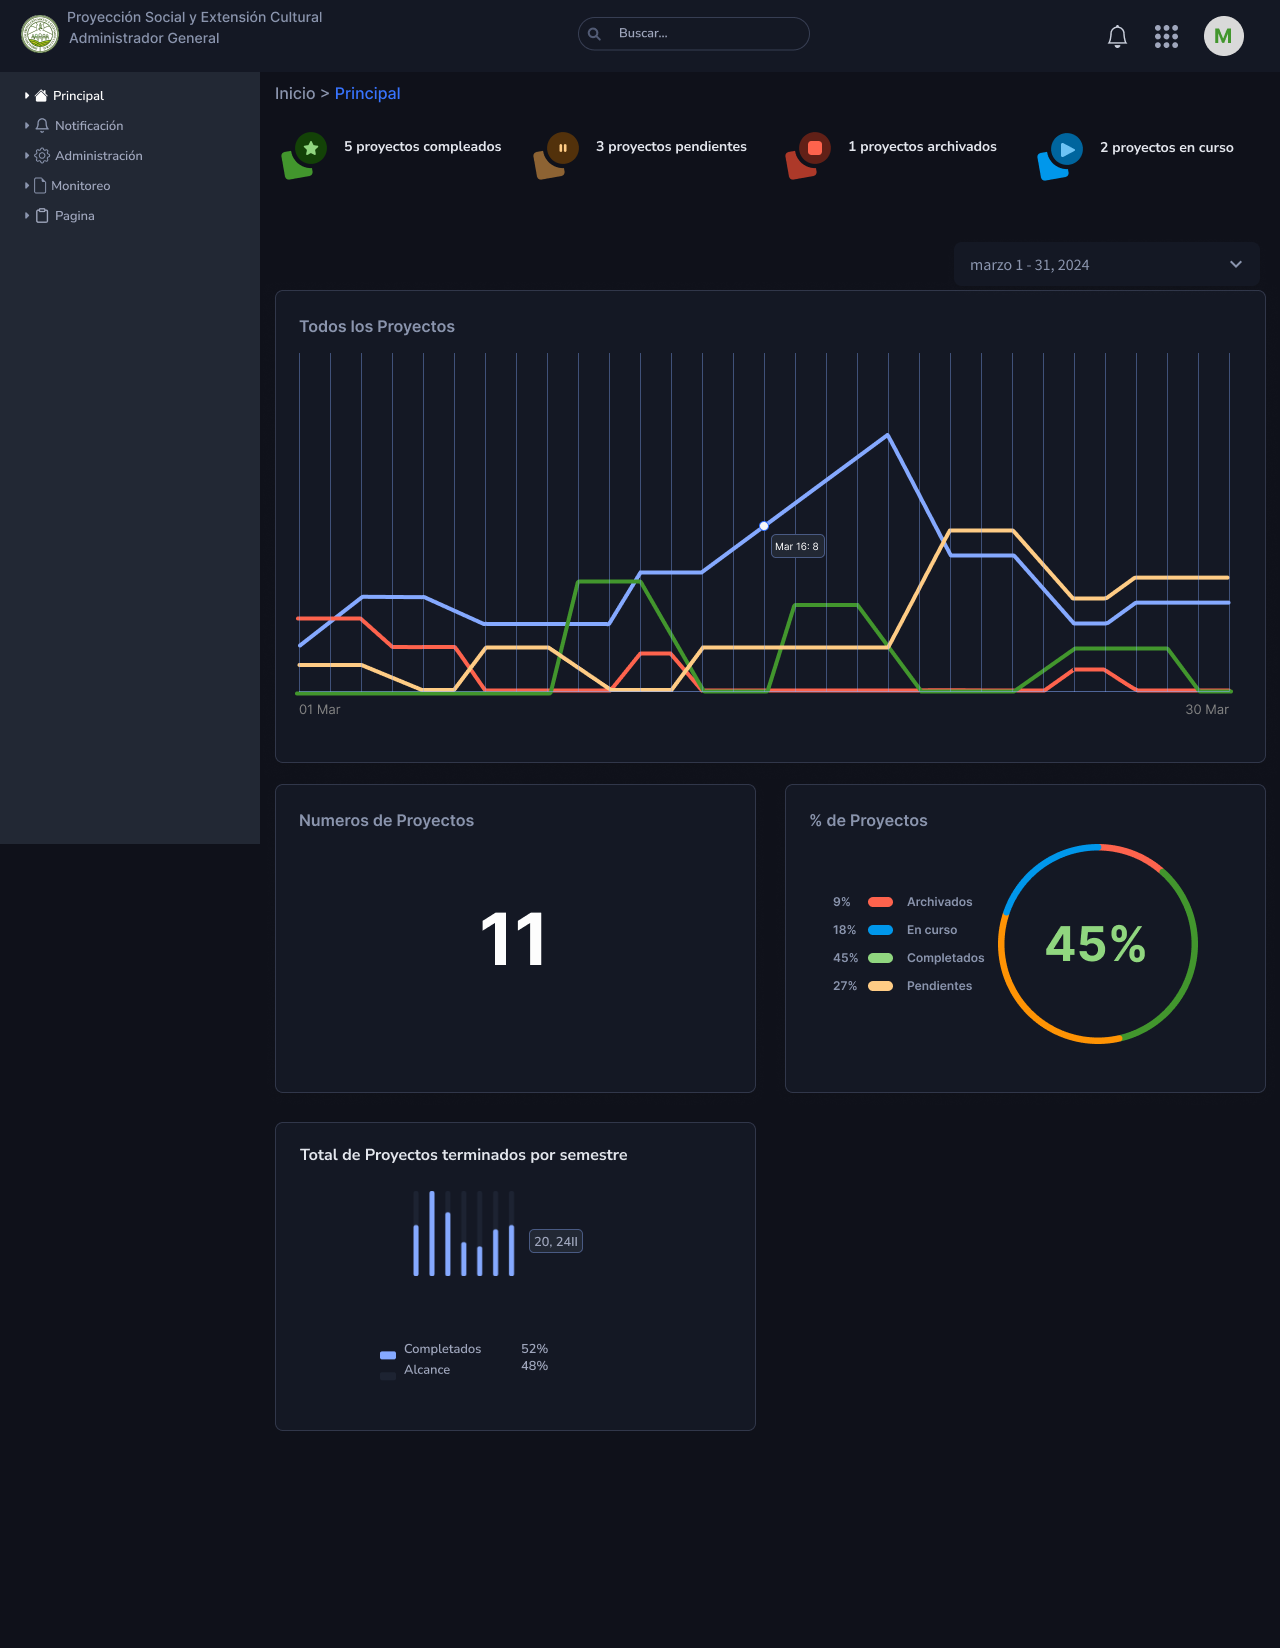
\includegraphics[width=0.8\textwidth]{assets/imagenes/principal.png}
    \label{fig:principal} 
\end{figure} 
\FloatBarrier

\begin{figure}[!htb] 
    \centering 
    \caption{Intranet - Vista de Proyectos} 
    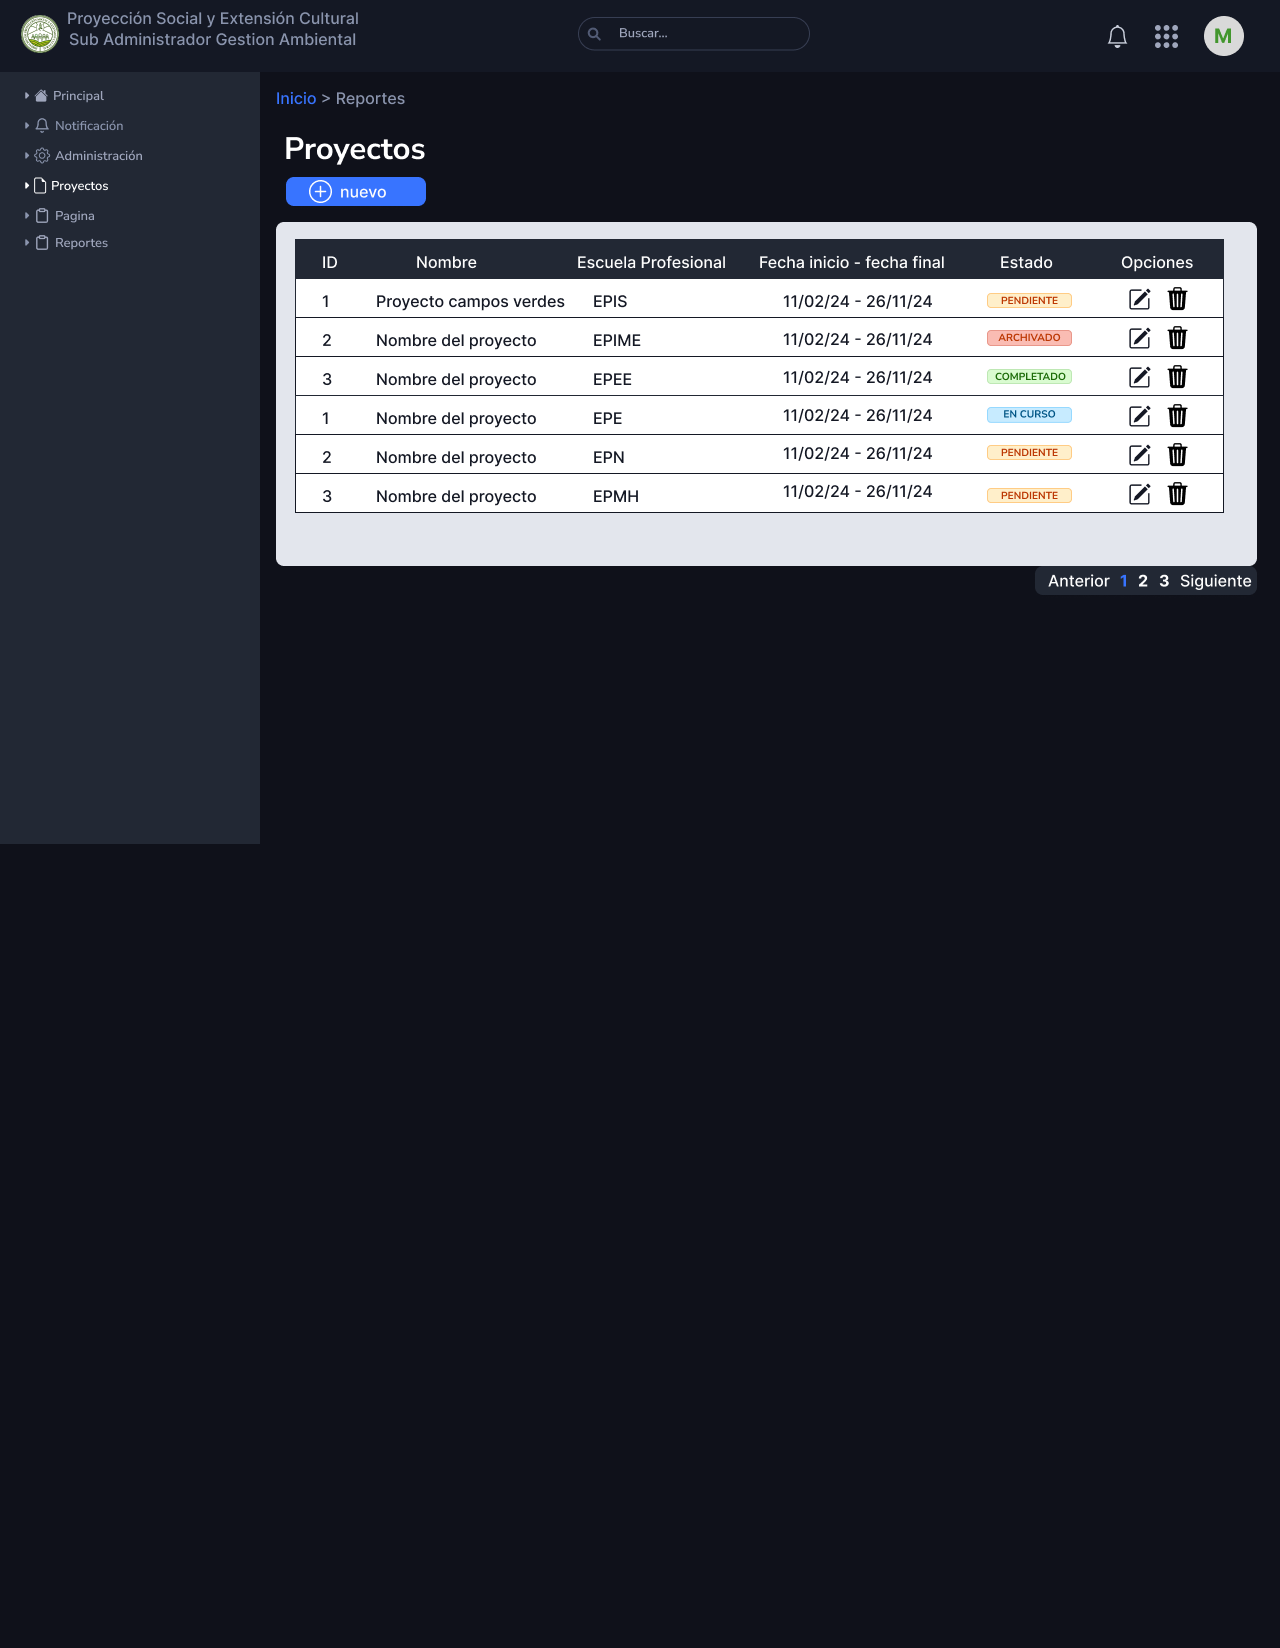
\includegraphics[width=0.8\textwidth]{assets/imagenes/proyectos.png}
    \label{fig:proyectos} 
\end{figure} 
\FloatBarrier

\begin{figure}[!htb] 
    \centering 
    \caption{Intranet - Vista de Administrador general del sistema} 
    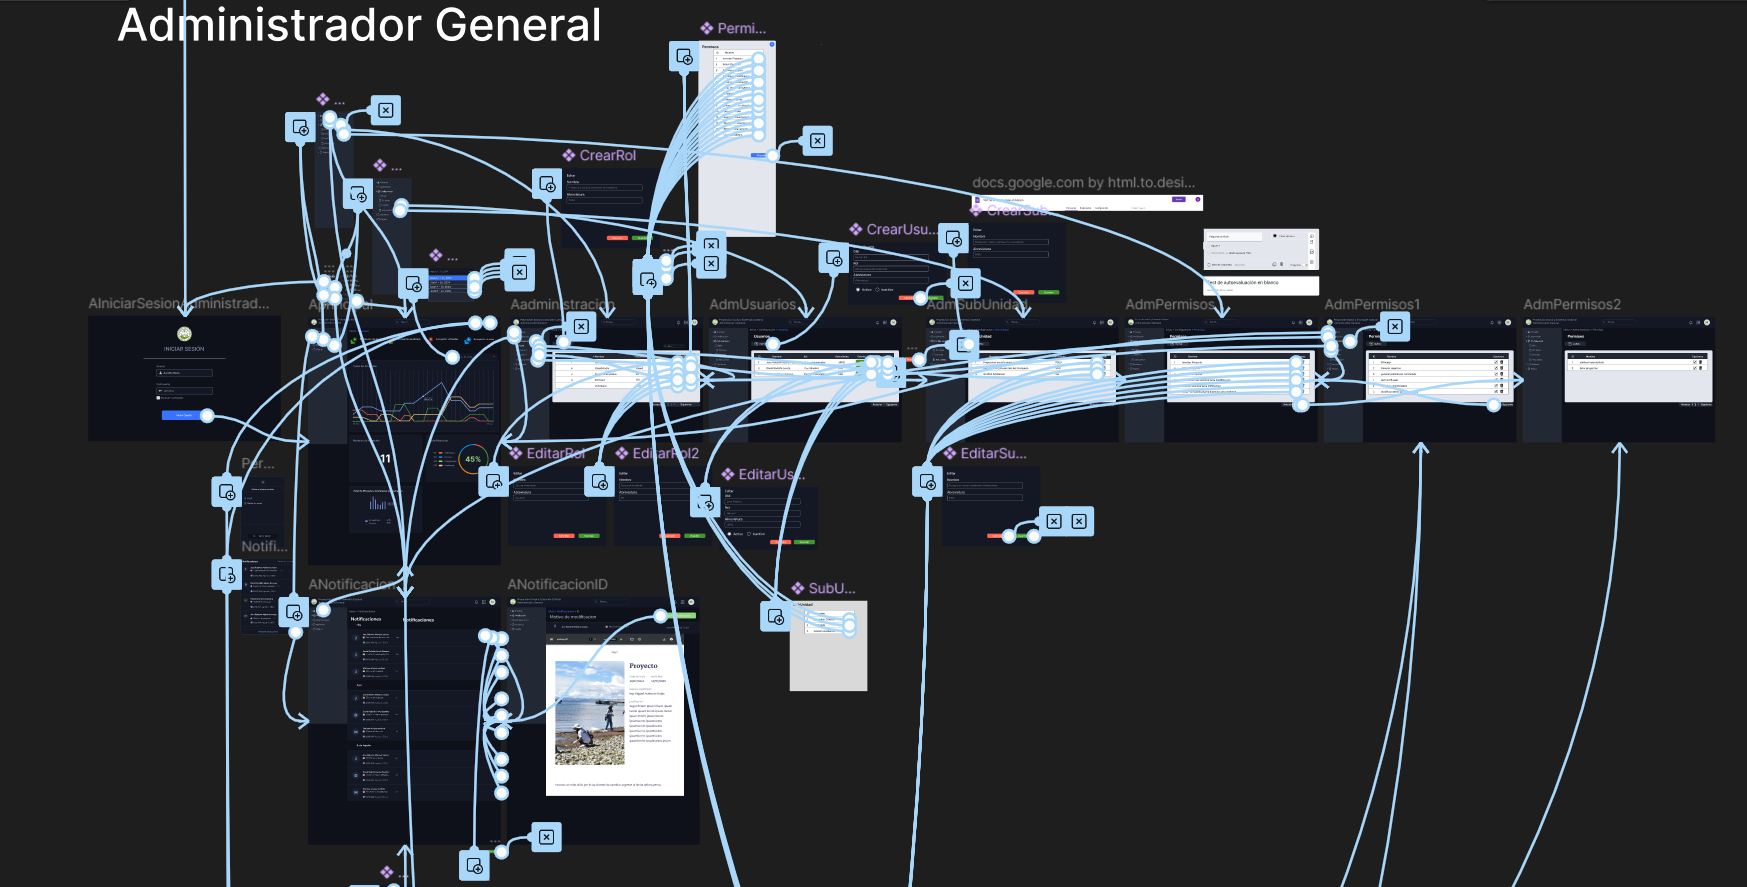
\includegraphics[width=0.8\textwidth]{assets/imagenes/figma_admin_general.png}
    \label{fig:admin_general} 
\end{figure} 
\FloatBarrier




\subsection{Actividad 3: Desarrollo del Backend}
\begin{longtable}{|p{5cm}|p{10cm}|}
    \caption{Resumen de la Actividad 3} \\ \hline
    \textbf{Responsable de la actividad} & \PracticanteNombre \\ \hline
    \textbf{Objetivo de la actividad} & Desarrollo Backend\\ \hline
    \textbf{Tareas realizadas} & 
    \begin{itemize}
        \item \textbf{Instalación de herramientas:} Node.js, Express, Prisma, PostgreSQL y Docker.
        \item \textbf{Configuración de repositorio:} Creación del repositorio en GitHub para control de versiones del sistema.
        \item \textbf{Servidor local:} Configuración de Node.js y Express para las comunicaciones con el backend a través de microservicios.
        \item \textbf{Base de datos:} Configuración inicial de PostgreSQL con Prisma.
        \item \textbf{Comunicación:} Creación de un enlace de Google Meet.
    \end{itemize} \\ \hline
    \textbf{Duración de la actividad} & 4 semanas \\ \hline
    \textbf{Fecha de inicio} & 01/06/25 \\ \hline
    \textbf{Fecha de culminación} & 30/06/25 \\ \hline
    \textbf{Materiales utilizados} & 
    \begin{itemize}
        \item Laptop Huawei Matebook D16 
        \item Visual Studio Code
        \item Terminal de Windows
        \item Google Meet
        \item GitHub
        \item postgreSQL
        \item Prisma
        \item TypeScript
        \item Node.js
        \item Express
    \end{itemize} \\ \hline
    \textbf{Resultados alcanzados} & Se programaron los endpoints de la API y se realizó el despliegue de la API en un servidor Docker local. \\ \hline
    \textbf{Porcentaje de avance} & 100\% \\ \hline
\end{longtable}
\FloatBarrier

\subsubsection{Detalles de la actividad}
El correcto instalado de herramientas asegura compatibilidad, productividad, y calidad del software, evitando errores técnicos. Facilita colaboración, pruebas, control de versiones y automatización, creando un entorno homogéneo y estable que agiliza el desarrollo y despliegue del proyecto.
%Enlace del fronted en GitHub \href{https://github.com/brahyanarch/frontend-next-dpsec.git}{https://github.com/brahyanarch/frontend-next-dpsec.git}
Enlace del Backend en GitHub \href{https://github.com/brahyanarch/DpsecGenseg.git}{https://github.com/brahyanarch/DpsecGenseg.git}




\begin{figure}[!htb] 
    \centering 
    \caption{Proyecto en Node.js con Express} 
    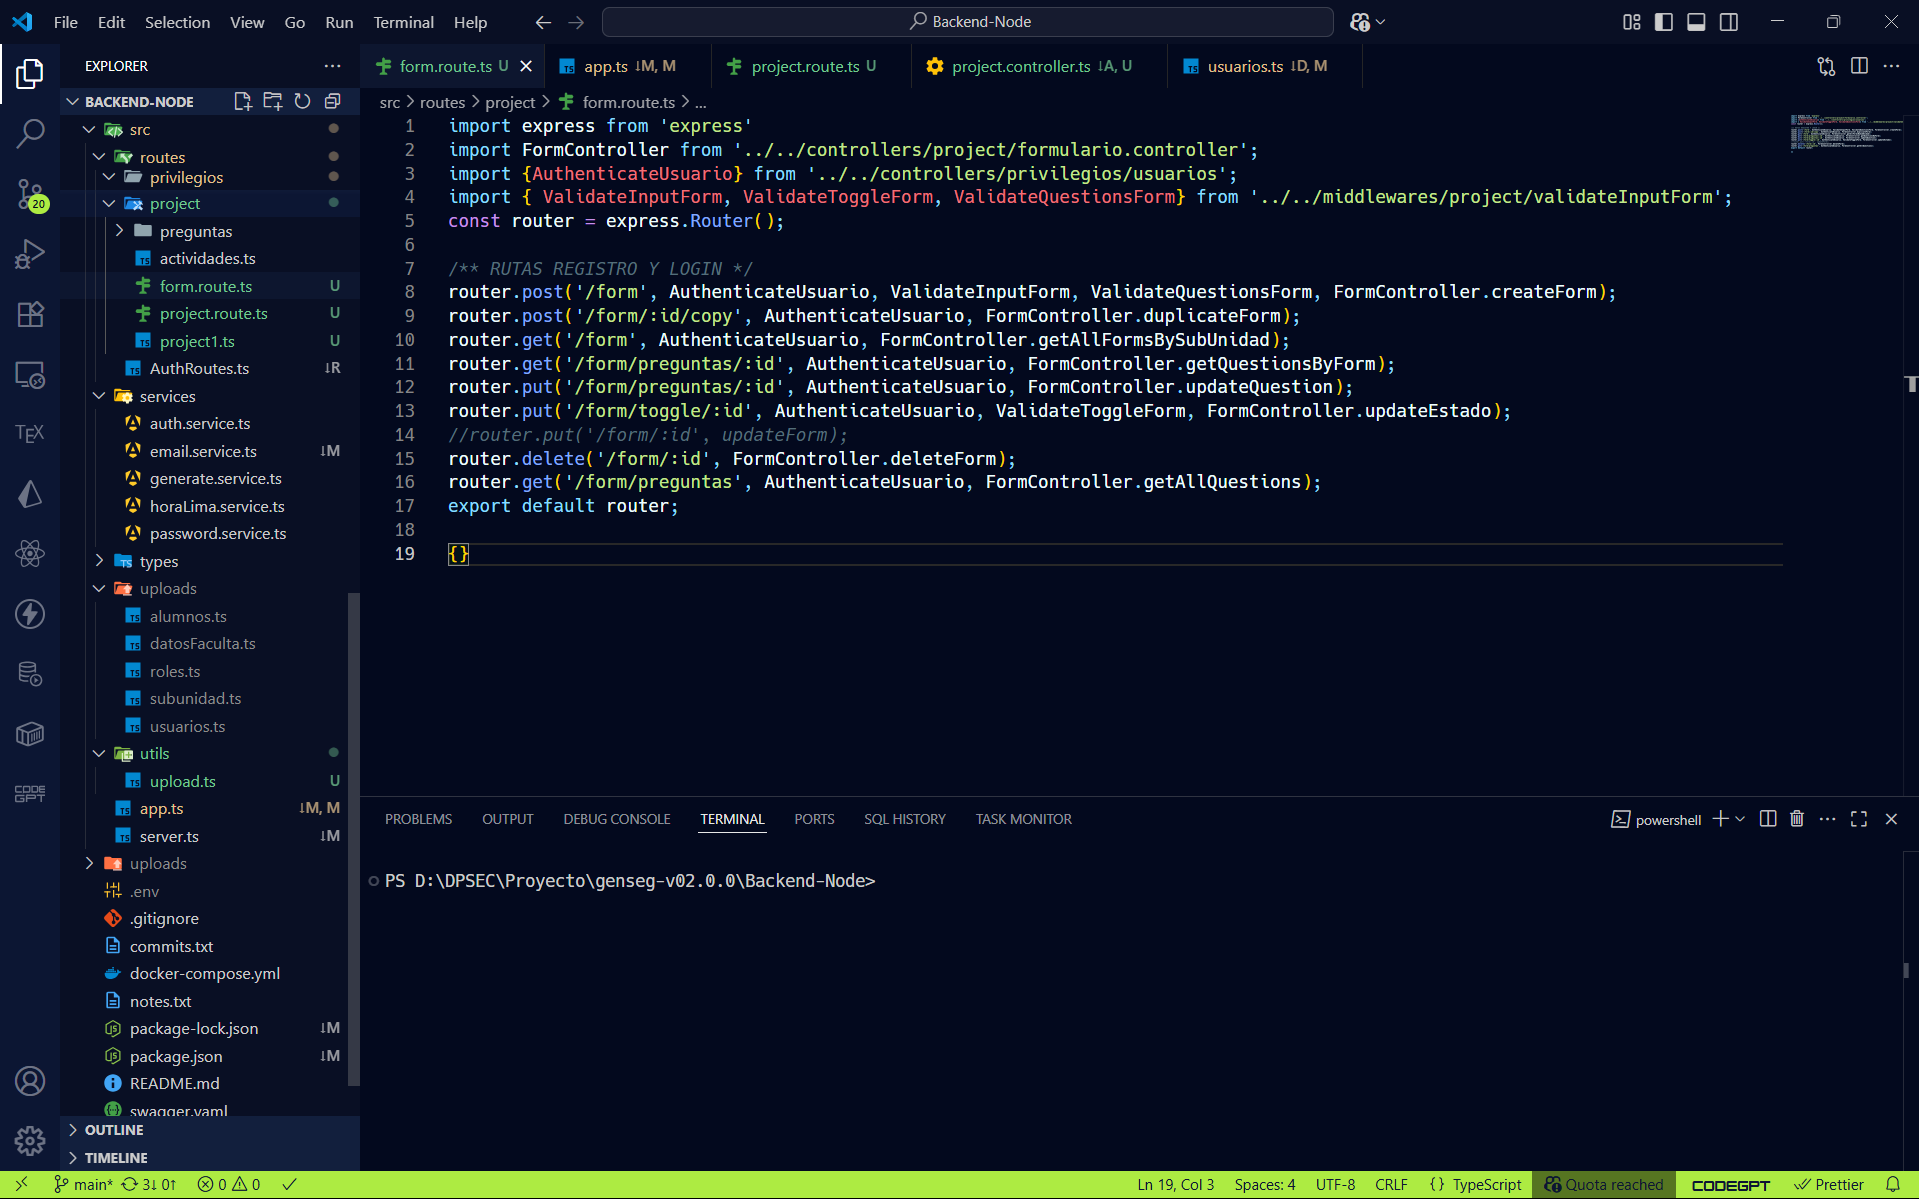
\includegraphics[width=0.9\textwidth]{assets/imagenes/backend.png}
    \label{fig:next} 
\end{figure} 
\FloatBarrier

\begin{figure}[!htb] 
    \centering 
    \caption{Creacion de routes, middlewares y controladores} 
    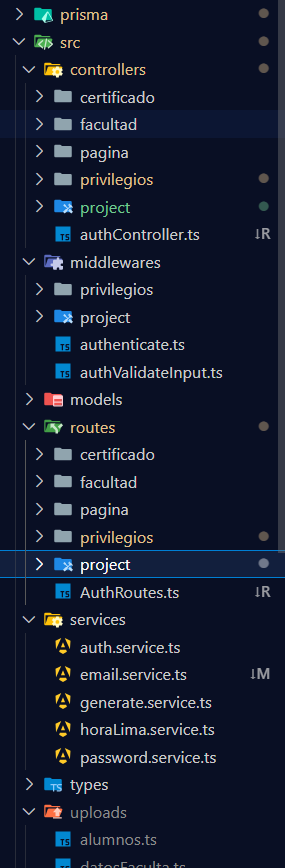
\includegraphics[width=0.2\textwidth]{assets/imagenes/proyecto_backend.png}
    \label{fig:backend} 
\end{figure} 
\FloatBarrier

%\begin{figure}[!htb] 
%    \centering 
%    \caption{Todo okey para trabajar en Next.js} 
%    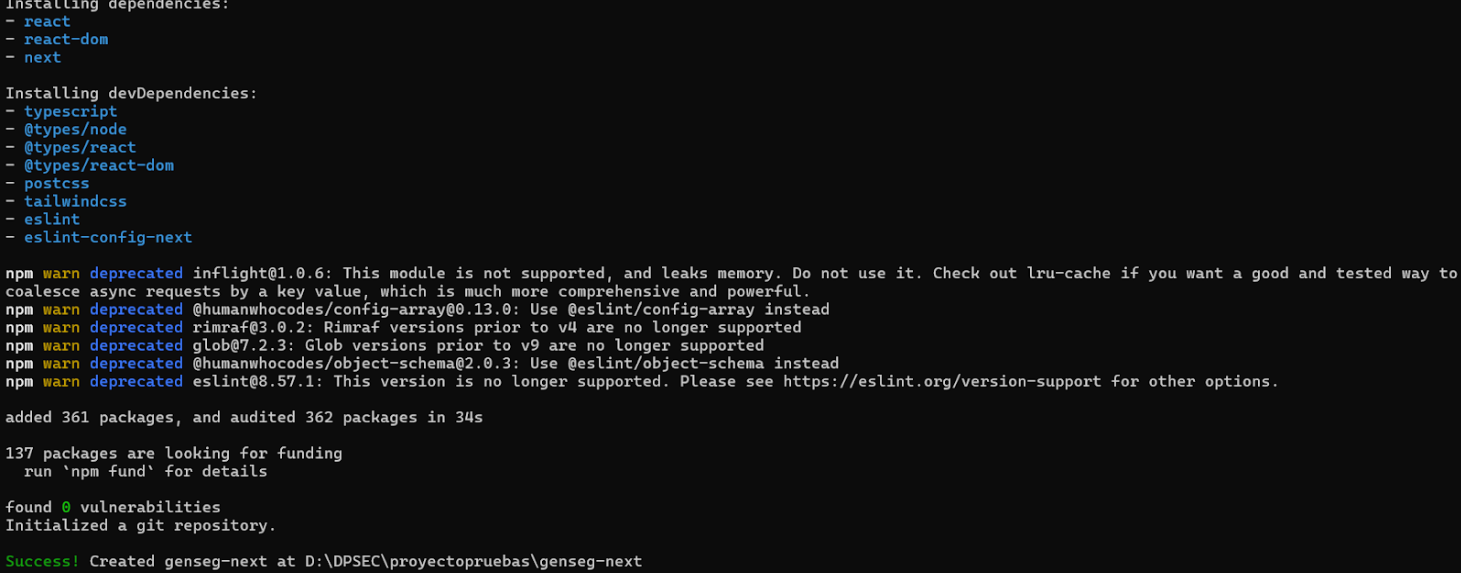
\includegraphics[width=0.8\textwidth]{assets/imagenes/next_listo.png}
%    \label{fig:listo_next} 
%\end{figure} 
%\FloatBarrier


%\begin{lstlisting}[language=Python, caption=Inicializando el proyecto en Next.js, label={lst:next}]
%        > npm run dev
%        
%        > project-genseg@0.1.0 dev
%        > next dev
%        
%         Port 3000 is in use, trying 3001 instead.
%         Next.js 14.2.9
%        - Local:        http://localhost:3001
%        - Environments: .env
%        
%         Starting...
%         Ready in 4.4s
%    \end{lstlisting}


%    \begin{figure}[!htb] 
%        \centering 
%        \caption{Ejecutando en el navegador} 
%        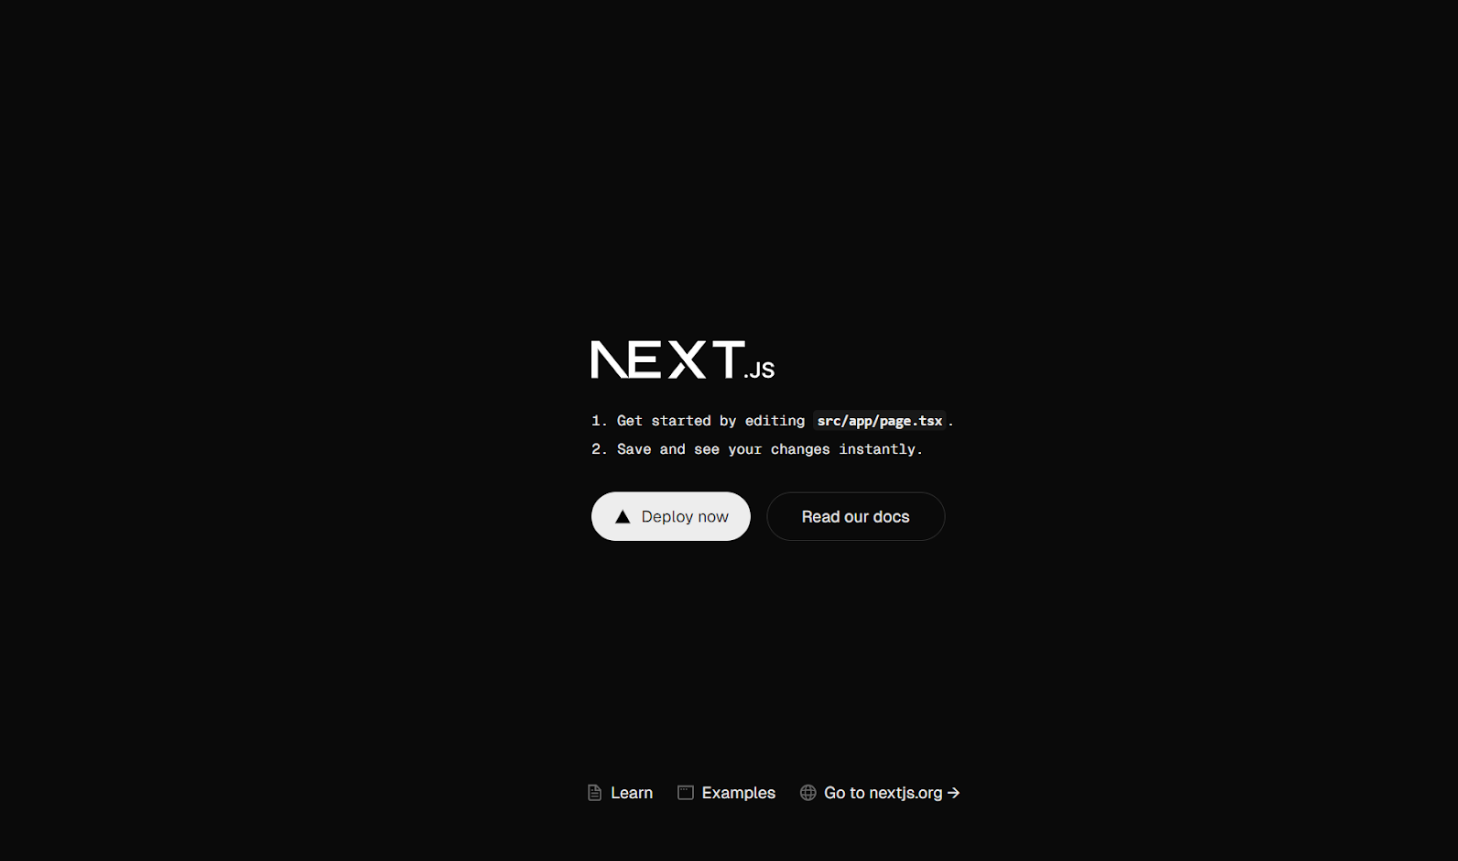
\includegraphics[width=0.8\textwidth]{assets/imagenes/init_next.png}
%        \label{fig:init_next} 
%    \end{figure} 
%    \FloatBarrier
%
%    \begin{figure}[!htb] 
%        \centering 
%        \caption{Codigo en Visual Studio Code} 
%        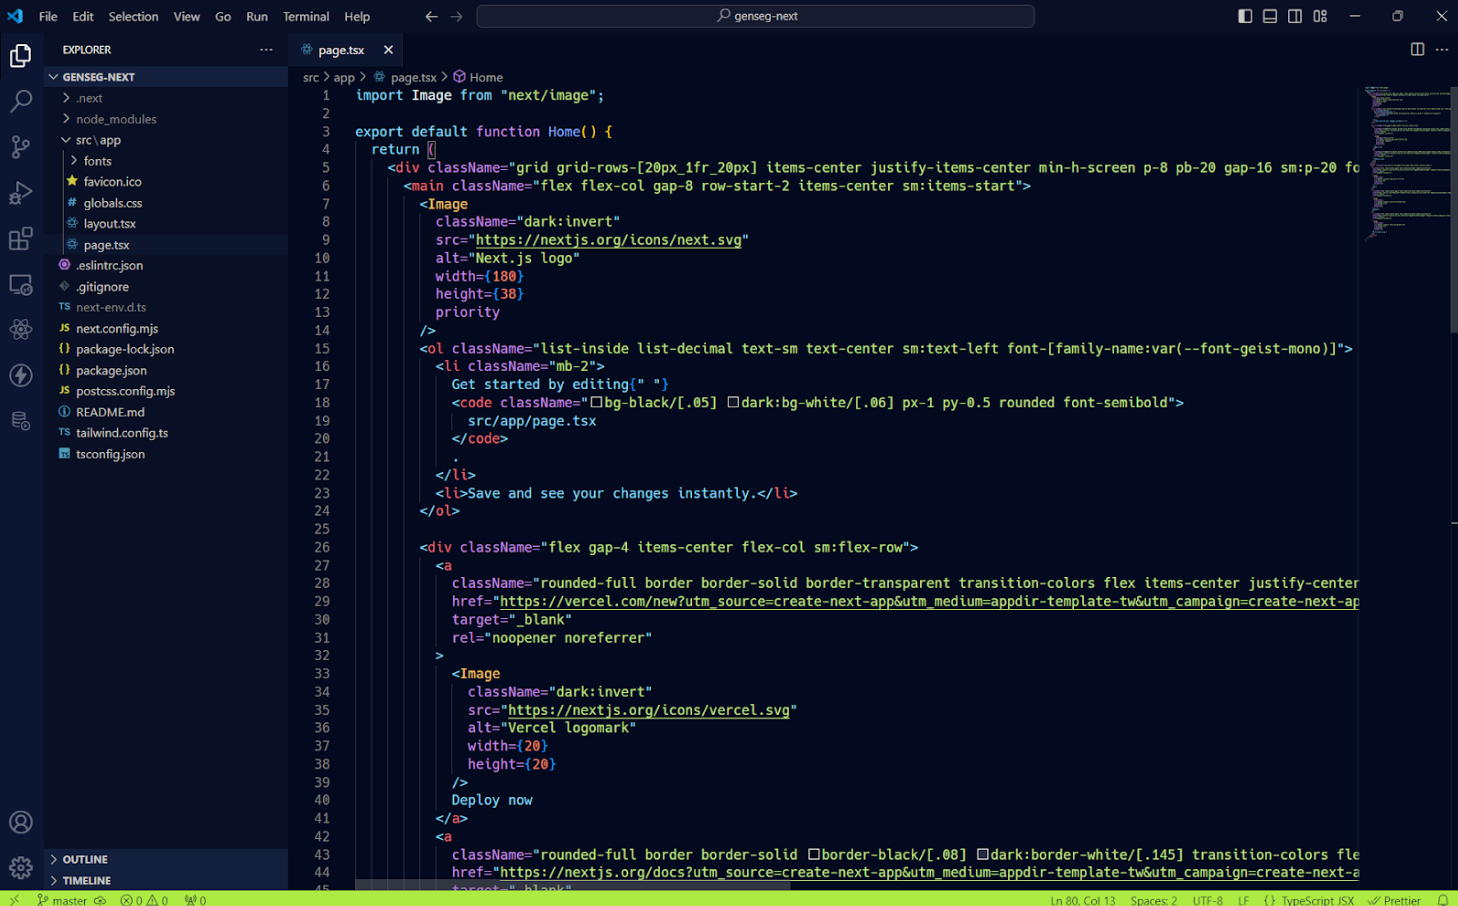
\includegraphics[width=0.8\textwidth]{assets/imagenes/vista_codigo.png}
%        \label{fig:codigo} 
%    \end{figure} 
%    \FloatBarrier



\subsection{Actividad 4: Desarrollo del Frontend (Interfaz de Usuario) }
\begin{table}[!htb]
    \centering
    \caption{Resumen de la Actividad 4}
    \begin{tabular}{|p{5cm}|p{10cm}|}
        \hline
        \textbf{Responsable de la actividad} & \PracticanteNombre \\ \hline
        \textbf{Objetivo de la actividad} & Desarrollo del
Frontend
(Interfaz de
Usuario) \\ \hline
        \textbf{Tareas realizadas} &
        \begin{itemize}
            \item Crear componentes o descargar si es necesario de shadcn (barra de navegación, pie de página) y rutas para la redirección.
            \item Crear la estructura de la pagina.
            \item Crear la pagina principal.
            \item Crear la interfaz de formularios
            \item Crear la interfaz de Proyectos
            \item Crear la interfaz de Usuarios
            \item Crear los pasos para subir proyectos
        \end{itemize} \\ \hline
        \textbf{Duración de la actividad} & 4 semanas \\ \hline
        \textbf{Fecha de inicio} & 01/07/25 \\ \hline
        \textbf{Fecha de culminación} & 31/07/25 \\ \hline
        \textbf{Materiales utilizados} &
        \begin{itemize}
            \item Laptop Huawei Matebook D16
            \item Visual Studio Code
            \item Terminal de Windows
            \item Google Meet
            \item GitHub
        \end{itemize} \\ \hline
        %\textbf{Detalles de la actividad (Fotos)} & [Incluye fotos relevantes aquí si las tienes] \\ \hline
        \textbf{Resultados alcanzados} & Programación del frontend (interfaz de usuario) \\ \hline
        \textbf{Porcentaje de avance} & 90\% \\ \hline
    \end{tabular}
    \label{tab:actividad3}
\end{table}
\FloatBarrier

\subsubsection{Detalles de la actividad}
Crear todo los componentes como esta en el diseño del figma y crear las rutas para la redirección, crear la estructura de la pagina, crear la pagina principal, crear la interfaz de formularios, crear la interfaz de Proyectos, crear la interfaz de Usuarios, crear los pasos para subir proyectos.


\subsubsection{Detalles de la actividad}
Siguiendo las buenas practicas de Next.js dice que deberias realizar un componente que debuelve al componente padre siguiente este paradigma creamos la pagina principal con sus componentes de navegador, encabezado, carrusel y sus modelos para cada sub unidad.
creamos esos componentes y lo colocamos con datos ficticios por el momento hasta que salga los enpoints de la parte de backend y poder conectarlo con el fronted.
Enlace del fronted en GitHub \href{https://github.com/brahyanarch/frontend-next-dpsec.git}{https://github.com/brahyanarch/frontend-next-dpsec.git}
Para comprobar en la parte de logs la parte de pagina principal.


\begin{figure}[!htb] 
    \centering 
    \caption{Configuracion de un nuevo proyecto en Next.js} 
    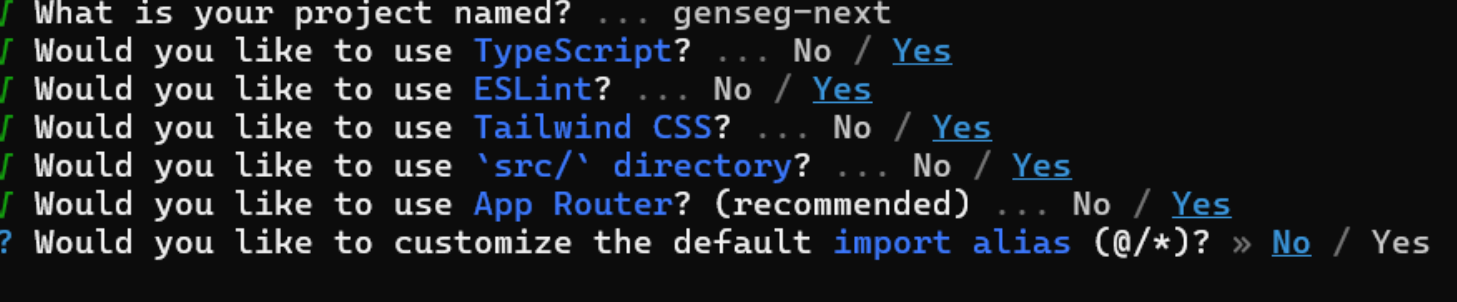
\includegraphics[width=0.8\textwidth]{assets/imagenes/config_next.png}
    \label{fig:config_next} 
\end{figure} 
\FloatBarrier

\begin{figure}[!htb] 
    \centering 
    \caption{Todo okey para trabajar en Next.js} 
    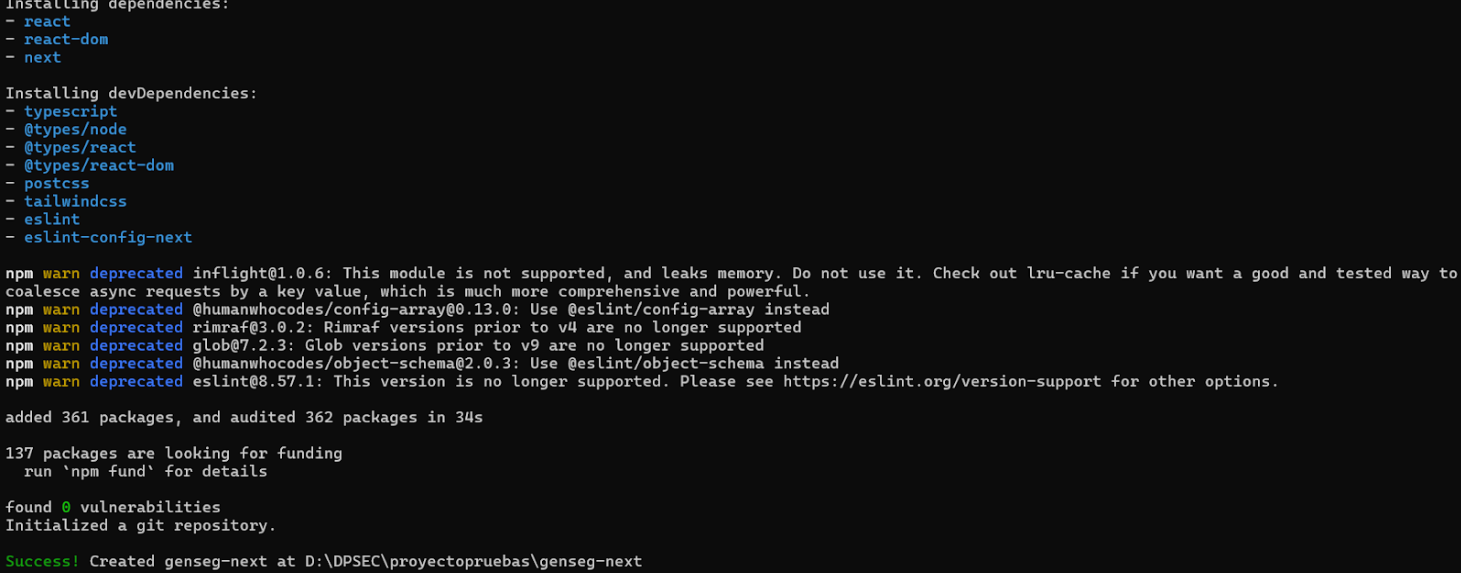
\includegraphics[width=0.8\textwidth]{assets/imagenes/next_listo.png}
    \label{fig:listo_next} 
\end{figure} 
\FloatBarrier


\begin{lstlisting}[language=Python, caption=Inicializando el proyecto en Next.js, label={lst:next}]
    > npm run dev
    
    > project-genseg@0.1.0 dev
    > next dev
    
    Port 3000 is in use, trying 3001 instead.
    Next.js 14.2.9
    - Local:        http://localhost:3001
    - Environments: .env
    
    Starting...
    Ready in 4.4s
\end{lstlisting}


\begin{figure}[!htb] 
    \centering 
    \caption{Ejecutando en el navegador} 
    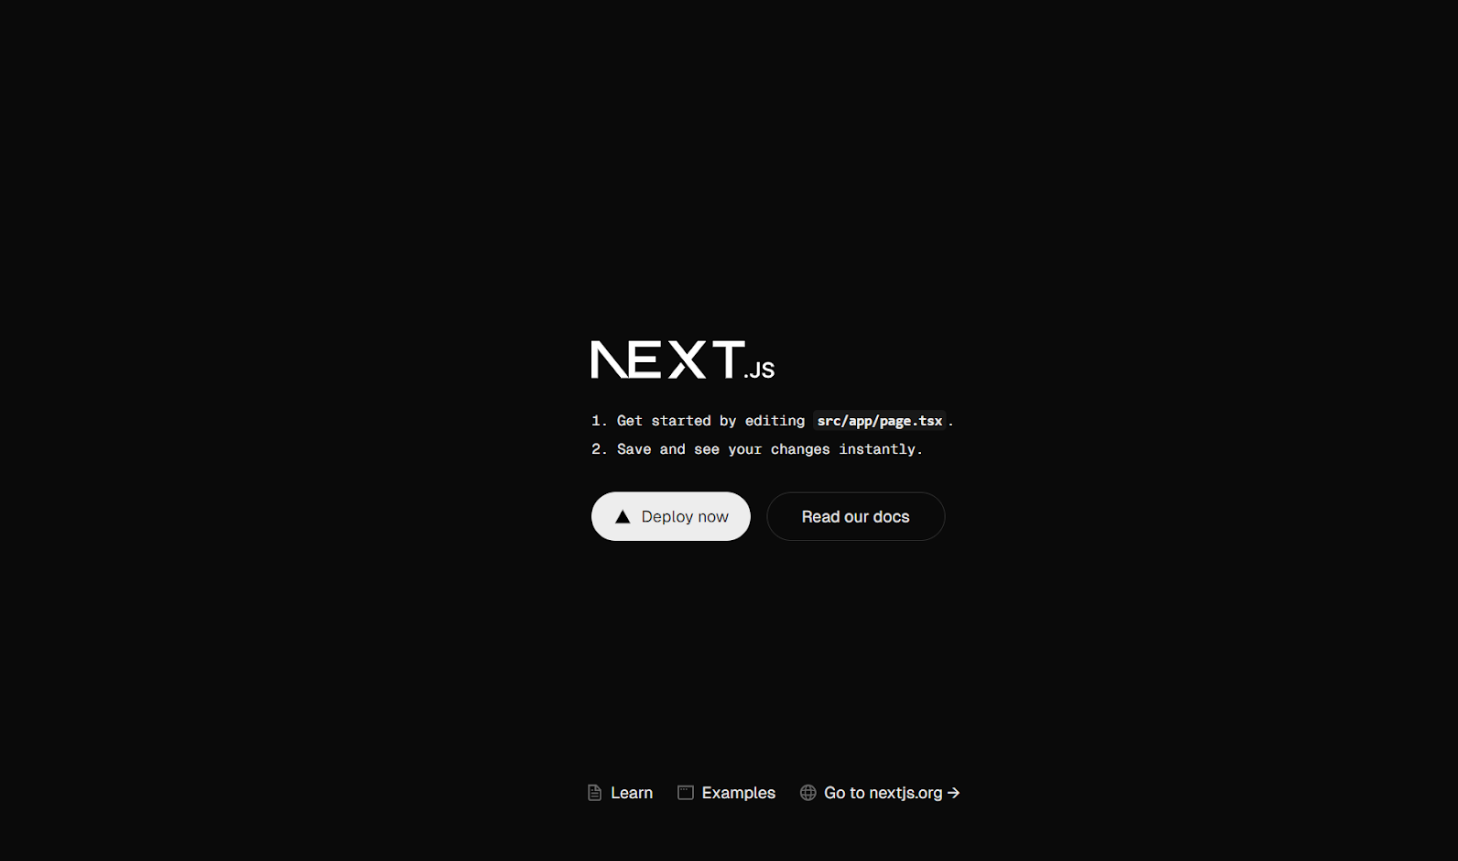
\includegraphics[width=0.8\textwidth]{assets/imagenes/init_next.png}
    \label{fig:init_next} 
\end{figure} 
\FloatBarrier

\begin{figure}[!htb] 
    \centering 
    \caption{Codigo en Visual Studio Code} 
    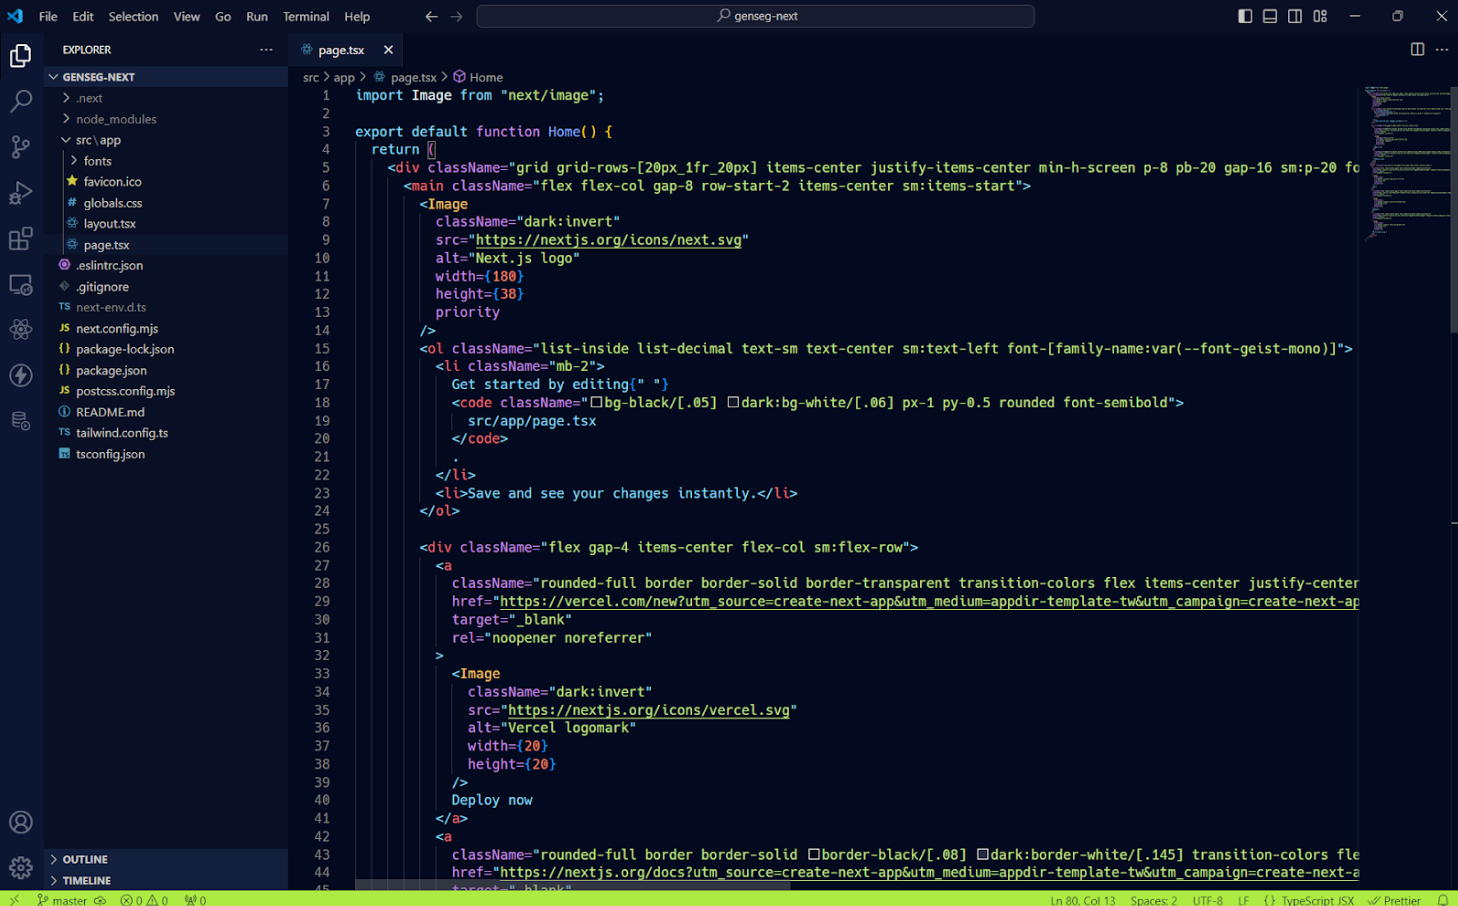
\includegraphics[width=0.8\textwidth]{assets/imagenes/vista_codigo.png}
    \label{fig:codigo} 
\end{figure} 
\FloatBarrier

\begin{figure}[!htb] 
    \centering 
    \caption{Pagina principal codificado} 
    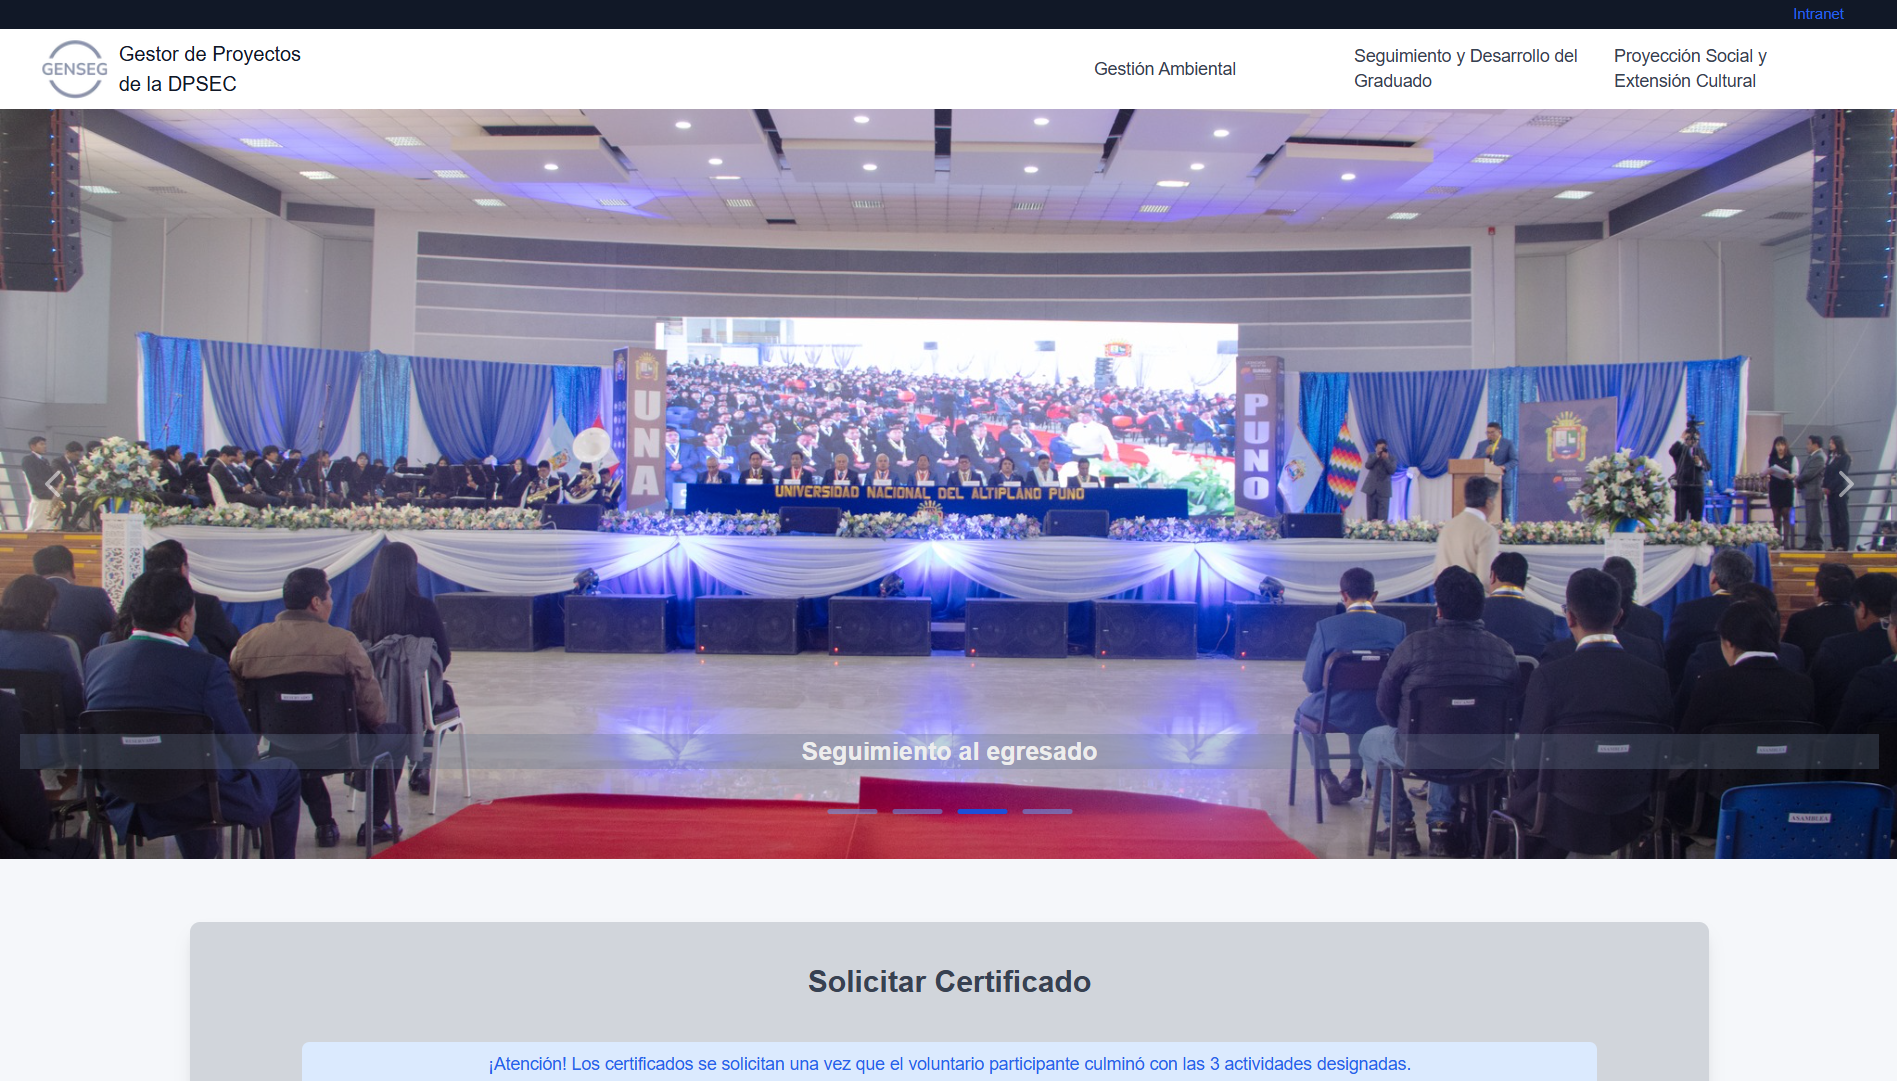
\includegraphics[width=0.8\textwidth]{assets/imagenes/paginaprincipalCodigo.png}
    \label{fig:pagina_codificado} 
\end{figure} 
\FloatBarrier


\begin{figure}[!htb] 
    \centering 
    \caption{Pagina login} 
    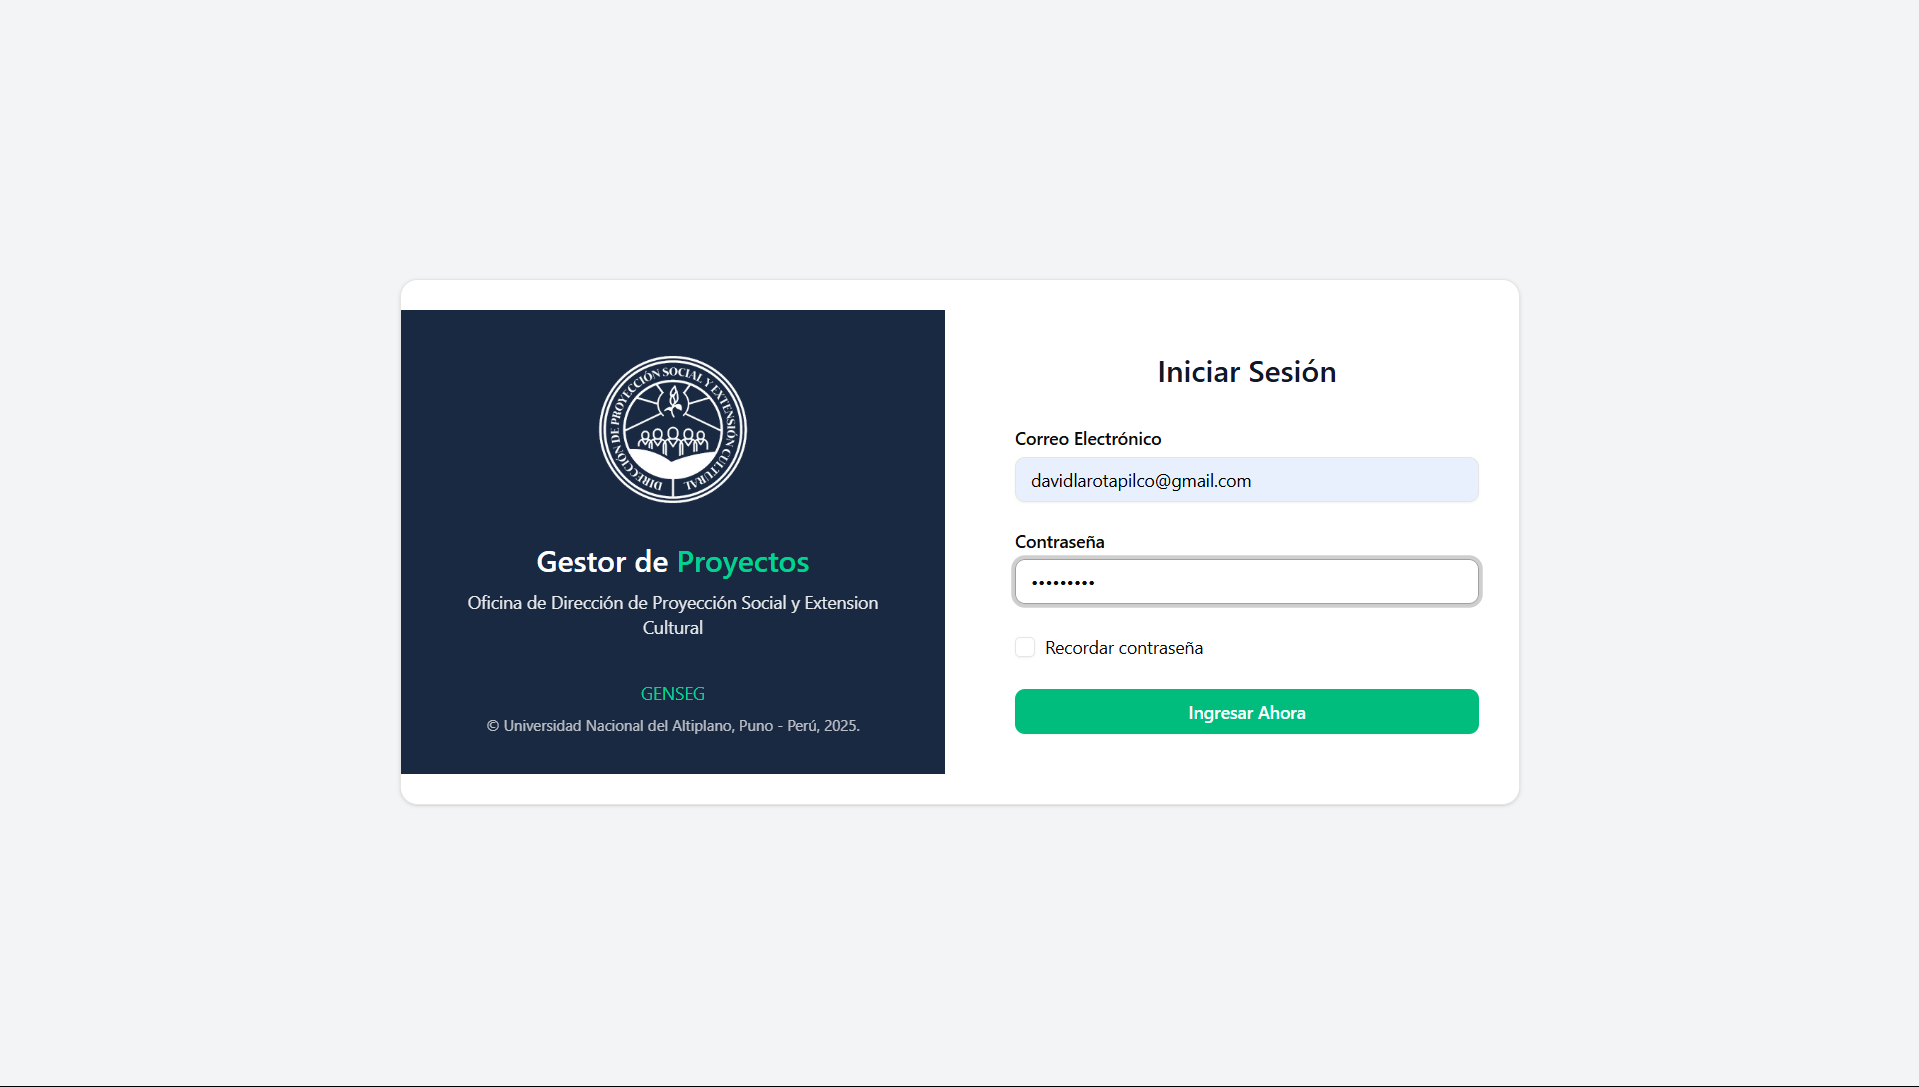
\includegraphics[width=0.8\textwidth]{assets/imagenes/login.png}
    \label{fig:login} 
\end{figure} 
\FloatBarrier

\begin{figure}[!htb] 
    \centering 
    \caption{Pagina escoger rol} 
    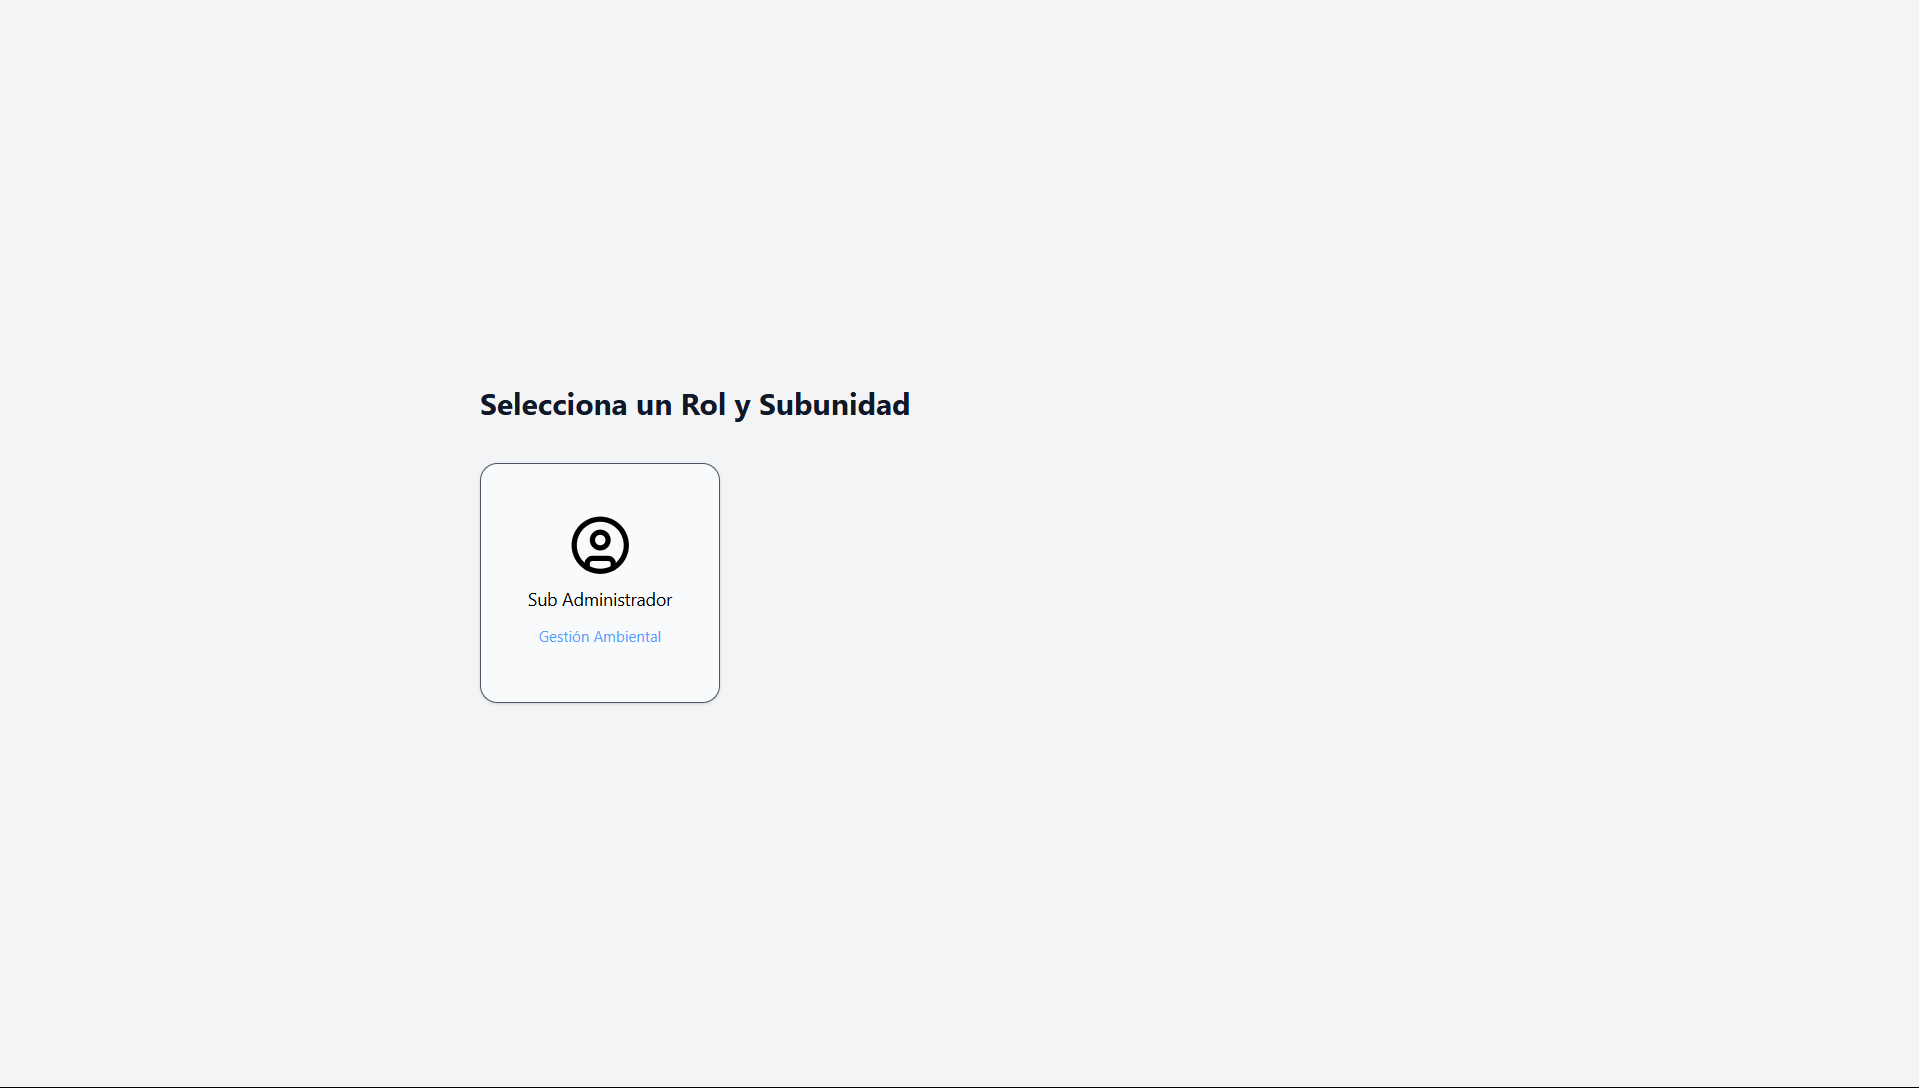
\includegraphics[width=0.8\textwidth]{assets/imagenes/rol.png}
    \label{fig:rol} 
\end{figure} 
\FloatBarrier
\begin{figure}[!htb] 
    \centering 
    \caption{Pagina para gestionar formularios} 
    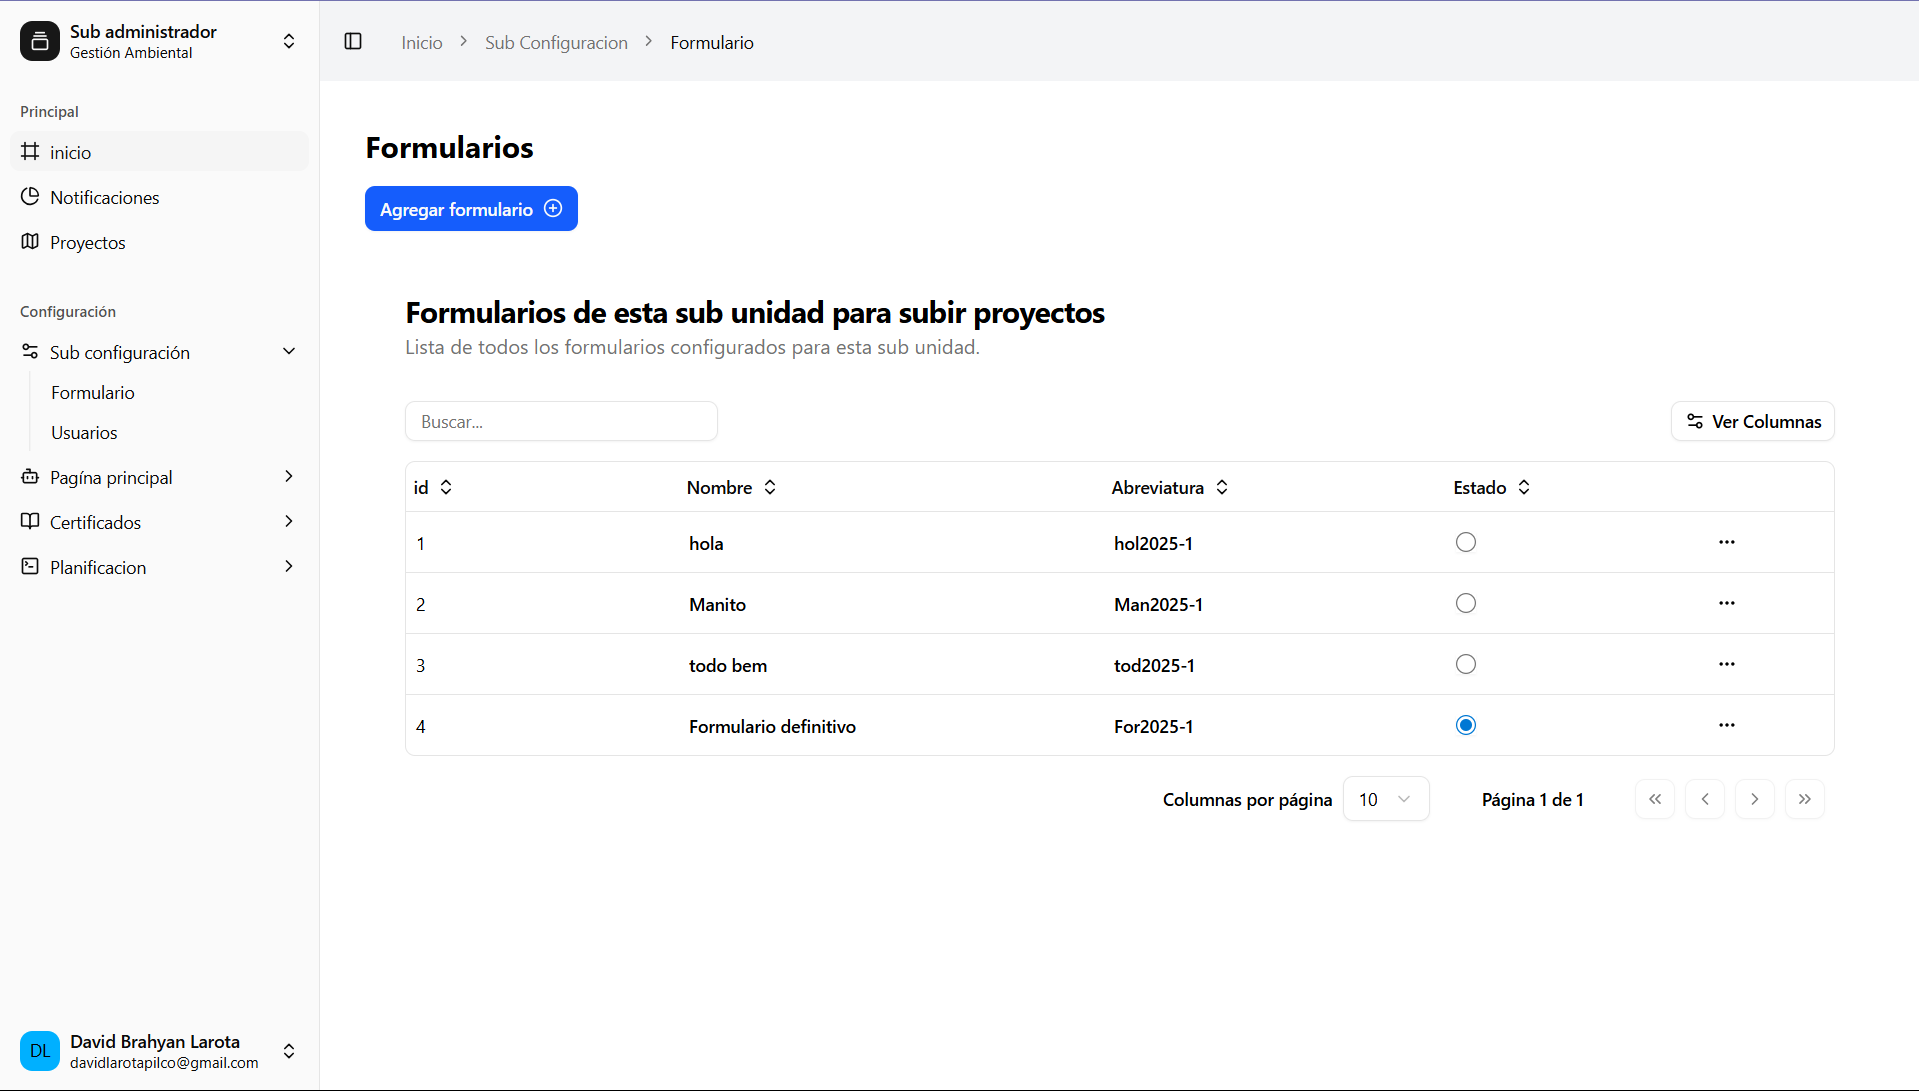
\includegraphics[width=0.8\textwidth]{assets/imagenes/formularios.png}
    \label{fig:formularios} 
\end{figure} 
\FloatBarrier
\begin{figure}[!htb] 
    \centering 
    \caption{Pagina para crear preguntas} 
    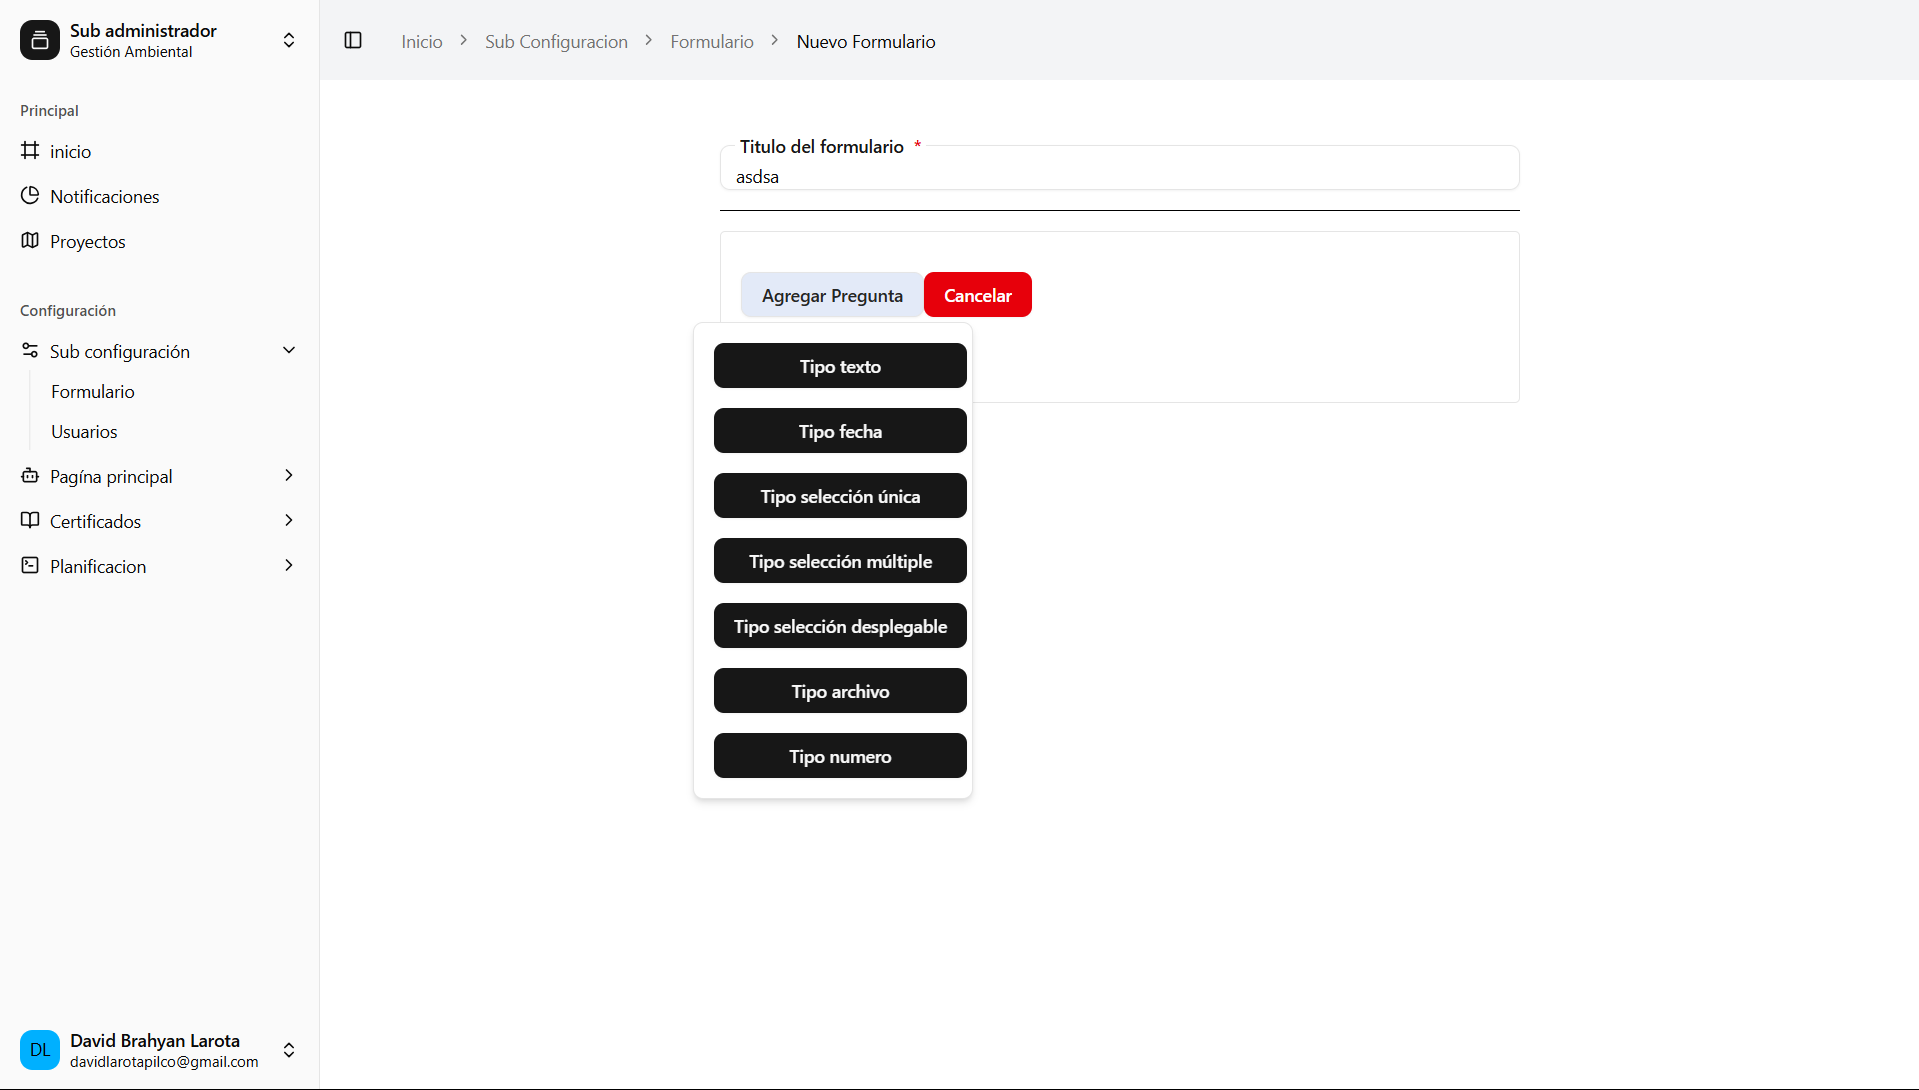
\includegraphics[width=0.8\textwidth]{assets/imagenes/preguntas.png}
    \label{fig:preguntas} 
\end{figure} 
\FloatBarrier
\begin{figure}[!htb] 
    \centering 
    \caption{Pagina para gestionar usuarios} 
    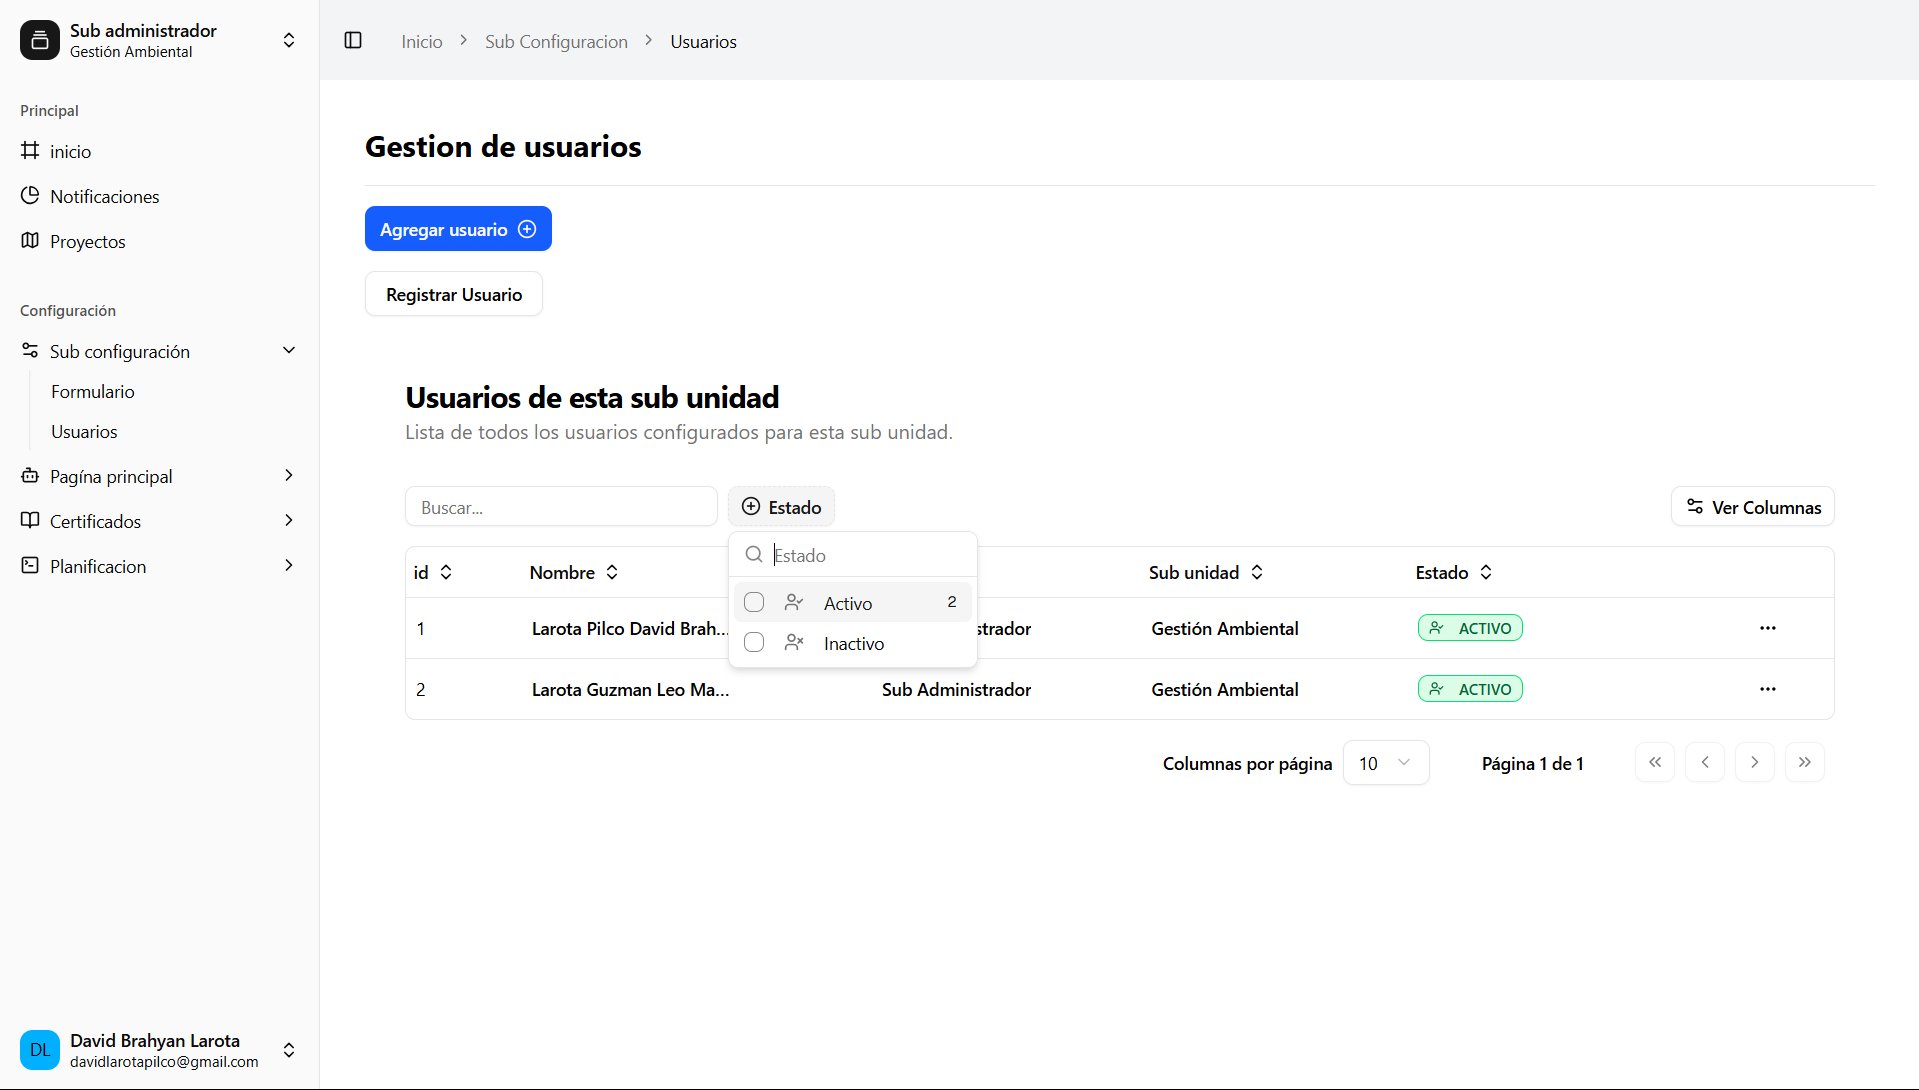
\includegraphics[width=0.8\textwidth]{assets/imagenes/usuarios.png}
    \label{fig:usuarios} 
\end{figure} 
\FloatBarrier
\begin{figure}[!htb] 
    \centering 
    \caption{Pagina para proyectos} 
    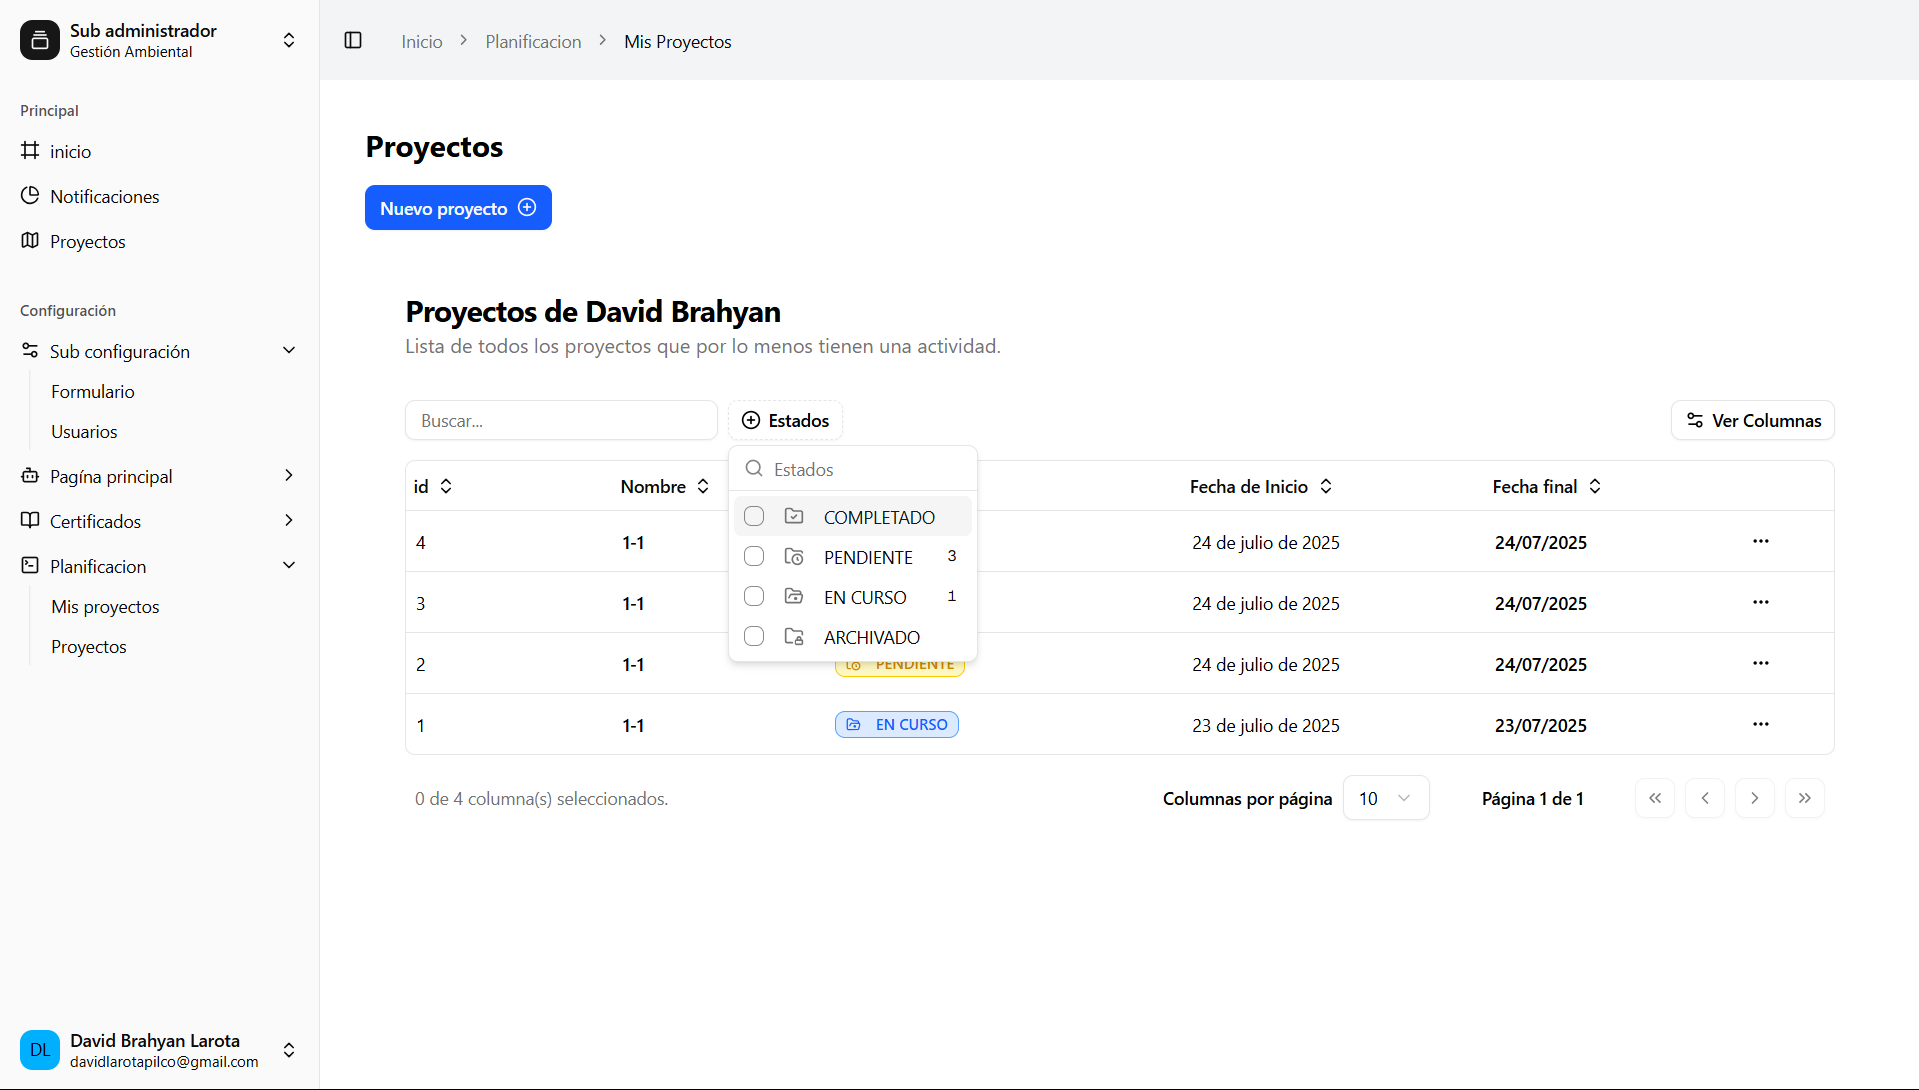
\includegraphics[width=0.8\textwidth]{assets/imagenes/proyectos_new.png}
    \label{fig:proyectos_page} 
\end{figure} 
\FloatBarrier
\begin{figure}[!htb] 
    \centering 
    \caption{Pagina para subir proyectos} 
    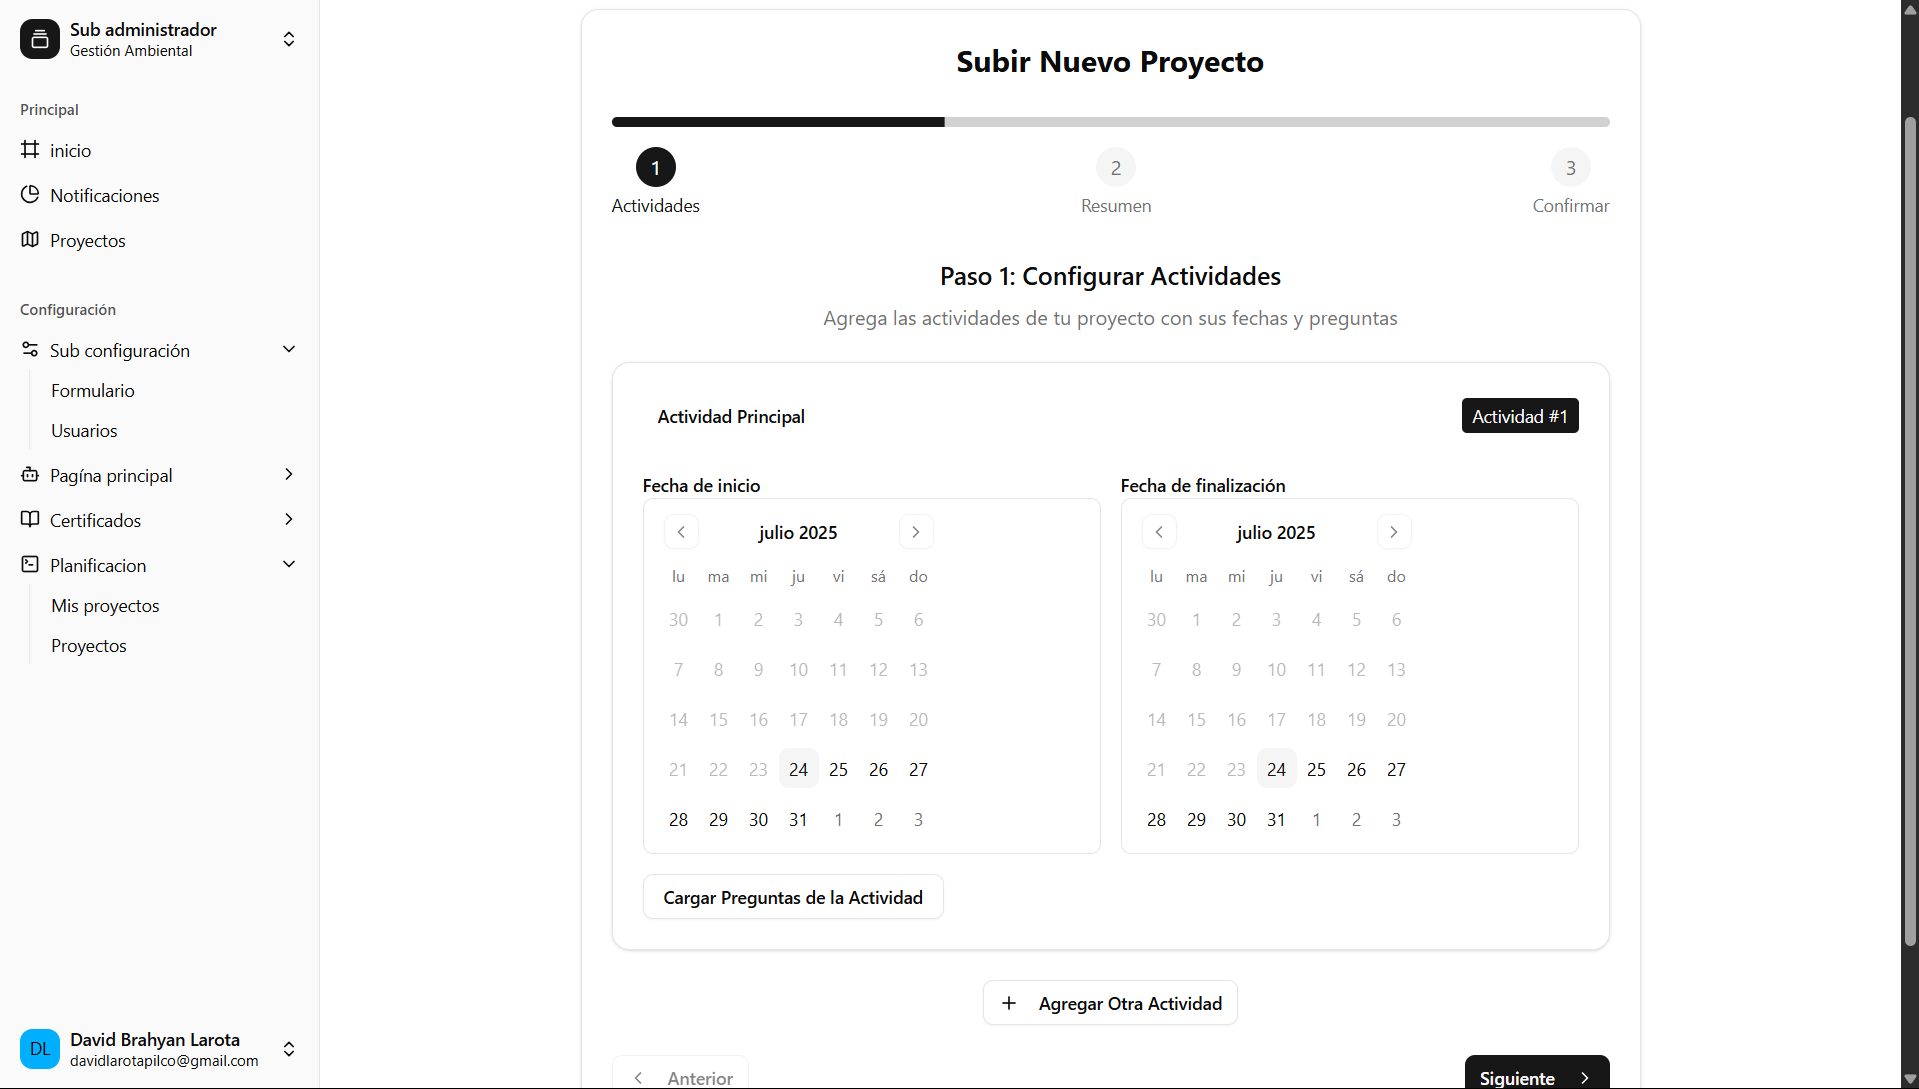
\includegraphics[width=0.8\textwidth]{assets/imagenes/subir_proyectos.png}
    \label{fig:subir_proyectos} 
\end{figure} 
\FloatBarrier
\begin{figure}[!htb] 
    \centering 
    \caption{Apartado de cuenta usuario} 
    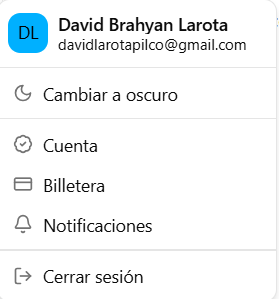
\includegraphics[width=0.8\textwidth]{assets/imagenes/cuenta.png}
    \label{fig:usuario} 
\end{figure} 
\FloatBarrier
\begin{figure}[!htb] 
    \centering 
    \caption{Soporte para modo oscuro} 
    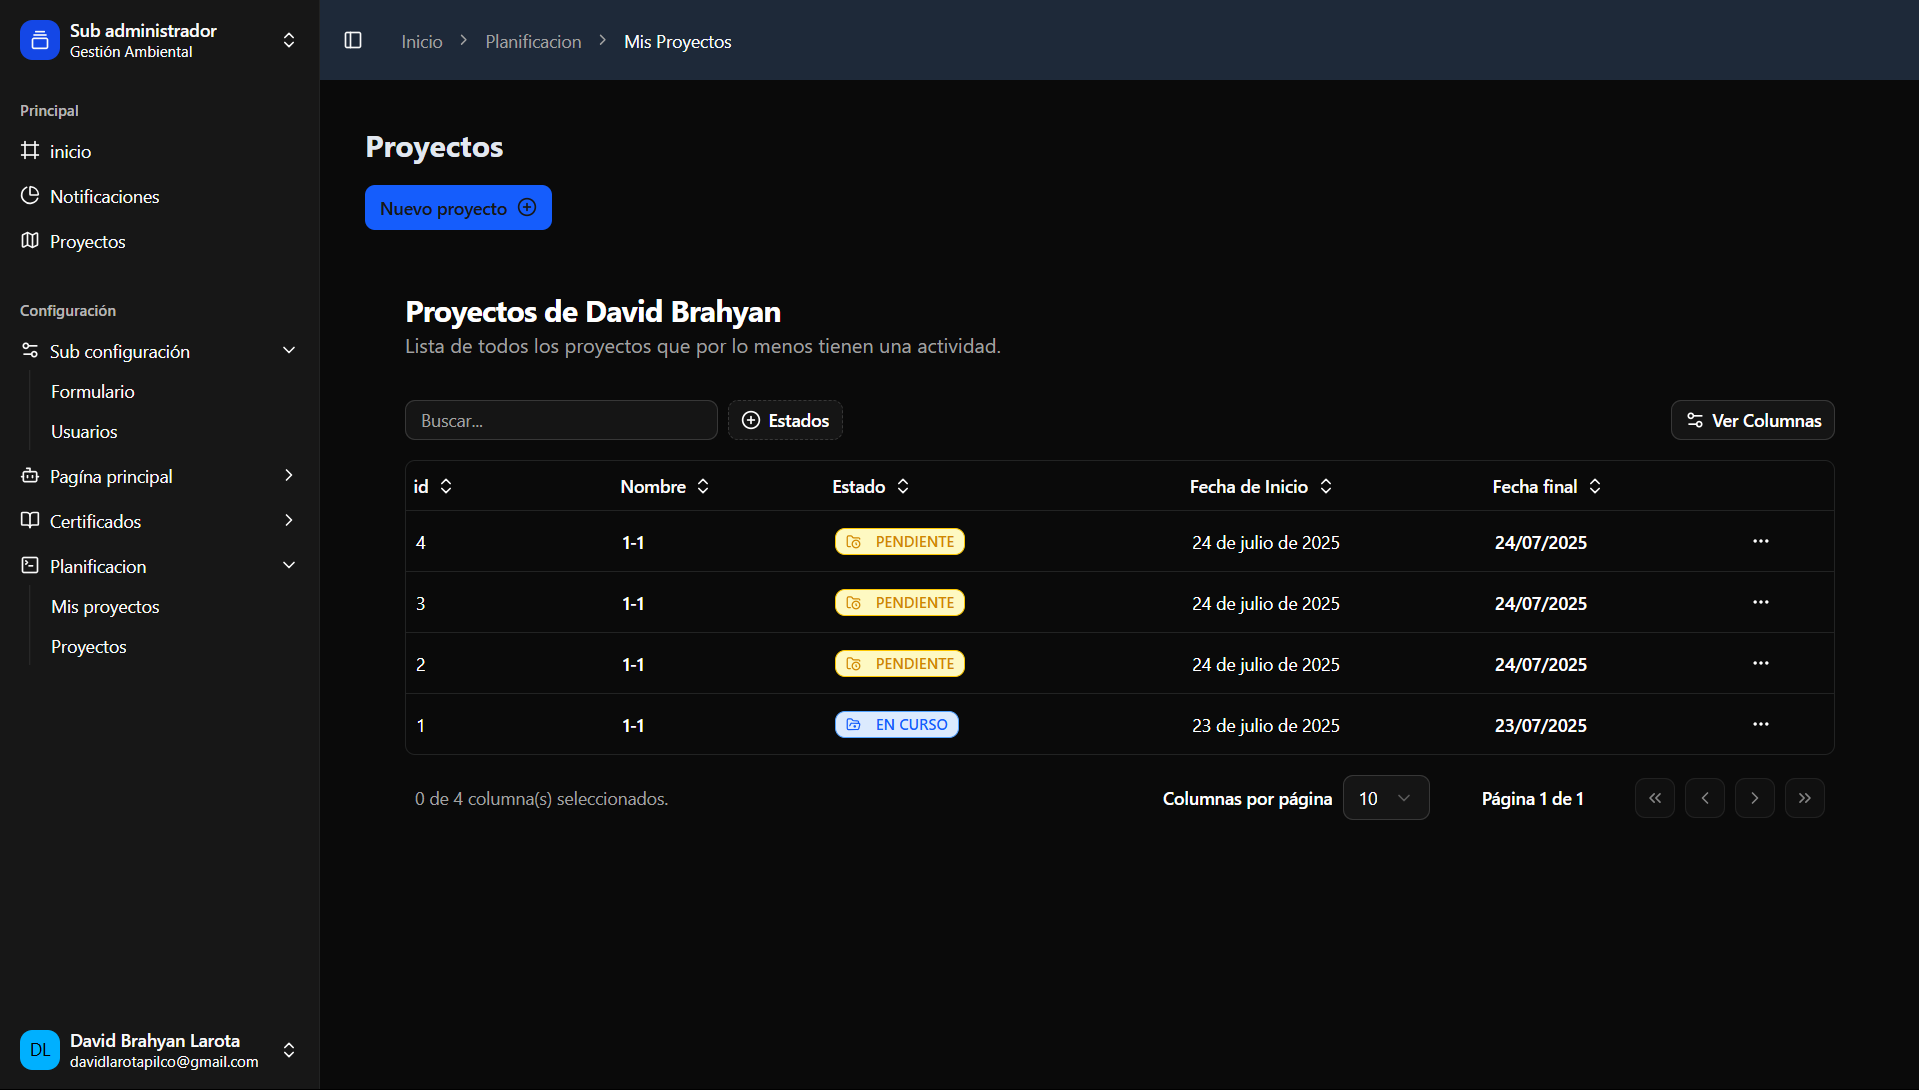
\includegraphics[width=0.8\textwidth]{assets/imagenes/modo_oscuro.png}
    \label{fig:modo_oscuro} 
\end{figure} 
\FloatBarrier



\subsection{Actividad 5: Pruebas
Unitarias y de
Integración }
\begin{table}[!htb]
    \centering
    \caption{Resumen de la Actividad 5}
    \begin{tabular}{|p{5cm}|p{10cm}|}
        \hline
        \textbf{Responsable de la actividad} & \PracticanteNombre \\ \hline
        \textbf{Objetivo de la actividad} & Pruebas
Unitarias y de
Integración \\ \hline
        \textbf{Tareas realizadas} &
        \begin{itemize}
            \item Realizar pruebas de caja blanca
            \item Realizar pruebas de caja navegador
            \item Realizar pruebas de seguridad
            \item Realizar pruebas de cifrado de datos.
        \end{itemize} \\ \hline
        \textbf{Duración de la actividad} & 2 semanas \\ \hline
        \textbf{Fecha de inicio} & 01/08/25 \\ \hline
        \textbf{Fecha de culminación} & 15/08/25 \\ \hline
        \textbf{Materiales utilizados} &
        \begin{itemize}
            \item Laptop Huawei Matebook D16
            \item Terminal de Windows
            \item Navegador Chrome
            \item GitHub
        \end{itemize} \\ \hline
        %\textbf{Detalles de la actividad (Fotos)} & [Incluye fotos relevantes aquí si las tienes] \\ \hline
        \textbf{Resultados alcanzados} & Solo se pudo realizar la seguridad y cifrado de datos y pruebas de caja blanca \\ \hline
        \textbf{Porcentaje de avance} & 40\% \\ \hline
    \end{tabular}
    \label{tab:actividad5}
\end{table}
\FloatBarrier

\subsubsection{Detalles de la actividad}
Se realizaron pruebas de tokens y de ataque por fuerza bruta; se protegieron el backend y el frontend, y se verificó el uso correcto de los tokens.



\subsection{Detalles de la actividad}
Capturas de pantalla donde se realizo las pruebas de seguridad evidencias de las rutas protegias acceso no autorizado.


\begin{figure}[!htb] 
    \centering 
    \caption{Pruebas en postman con tokens} 
    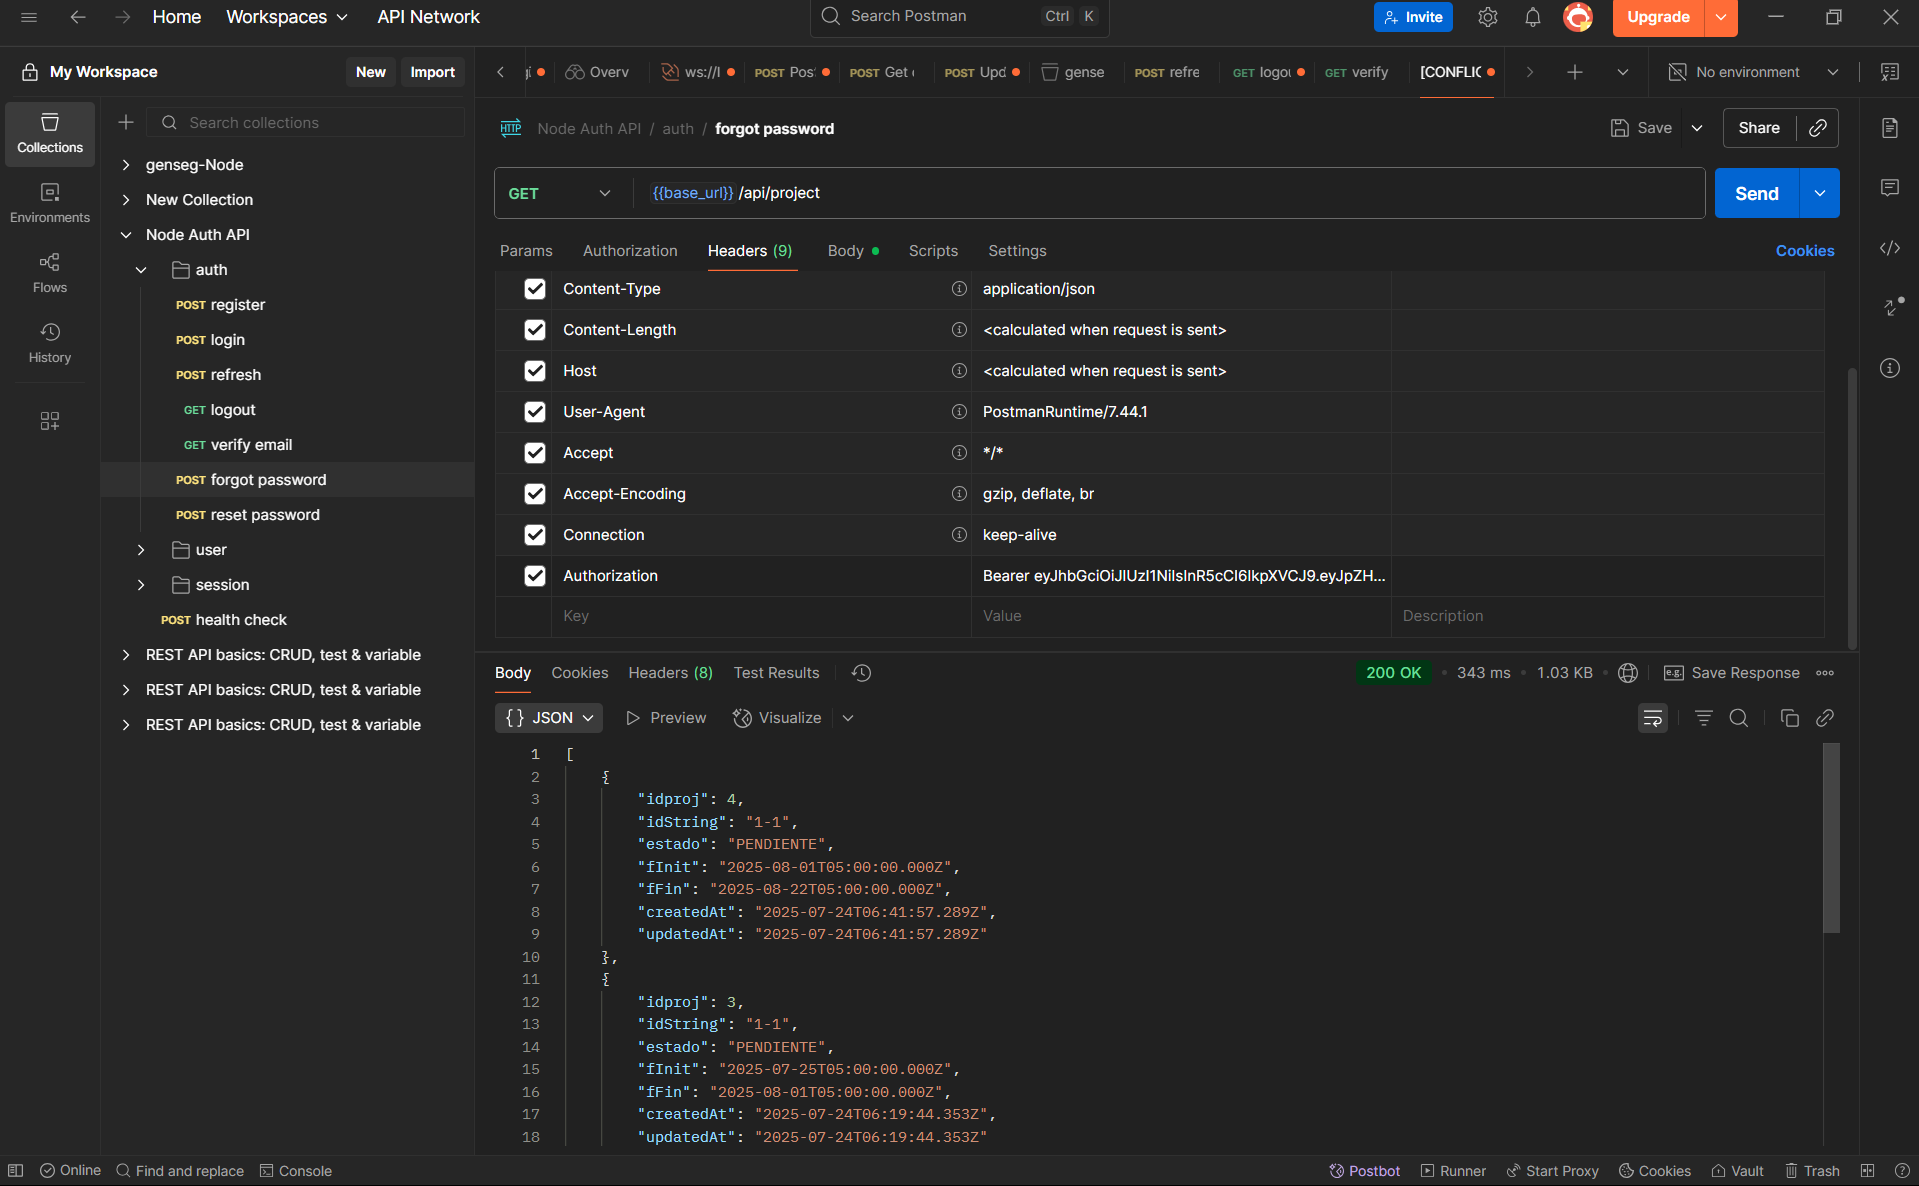
\includegraphics[width=0.8\textwidth]{assets/imagenes/postman.png}
    \label{fig:postman} 
\end{figure} 
\FloatBarrier


\begin{figure}[!htb] 
    \centering 
    \caption{Pruebas de postman con acceso no autorizado} 
    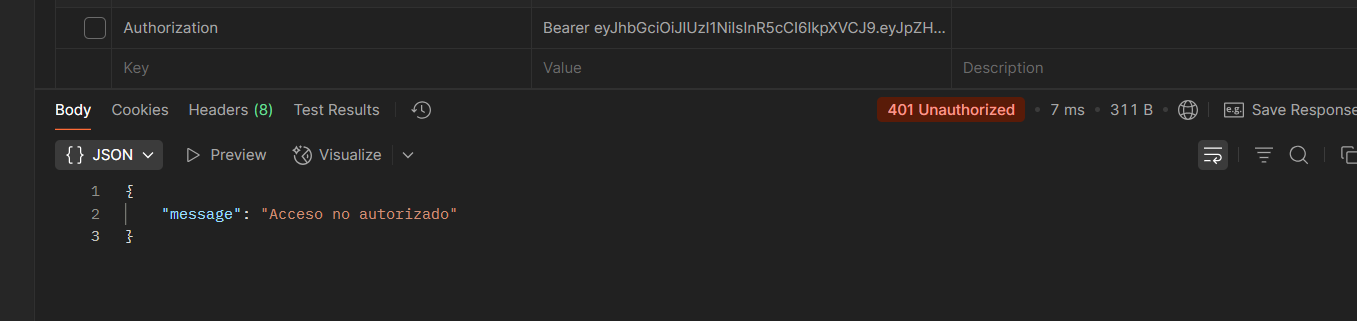
\includegraphics[width=0.8\textwidth]{assets/imagenes/postman1.png}
    \label{fig:postman1} 
\end{figure} 
\FloatBarrier

\begin{figure}[!htb] 
    \centering 
    \caption{Pruebas de la API protegida} 
    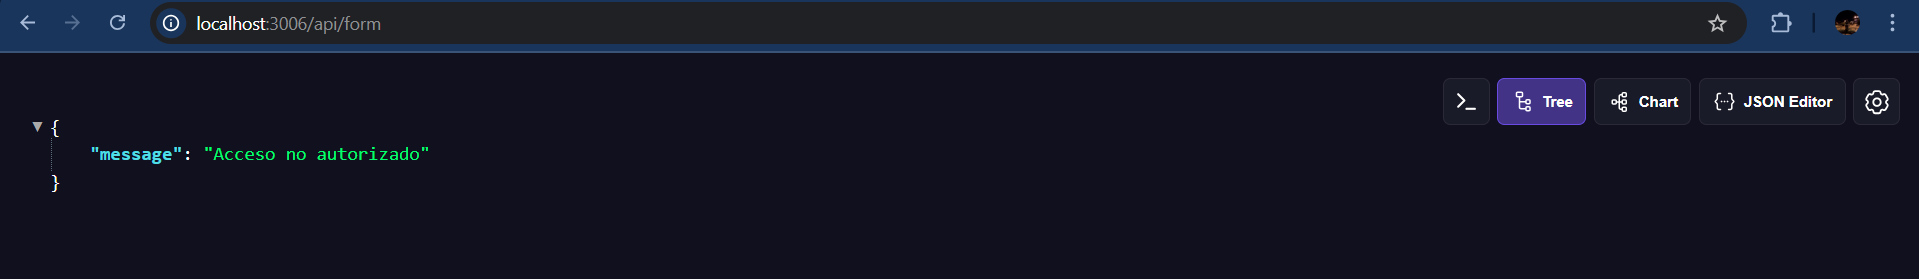
\includegraphics[width=0.8\textwidth]{assets/imagenes/api.png}
    \label{fig:api} 
\end{figure} 
\FloatBarrier

\begin{figure}[!htb] 
    \centering 
    \caption{Base de datos en DB Bearer CE } 
    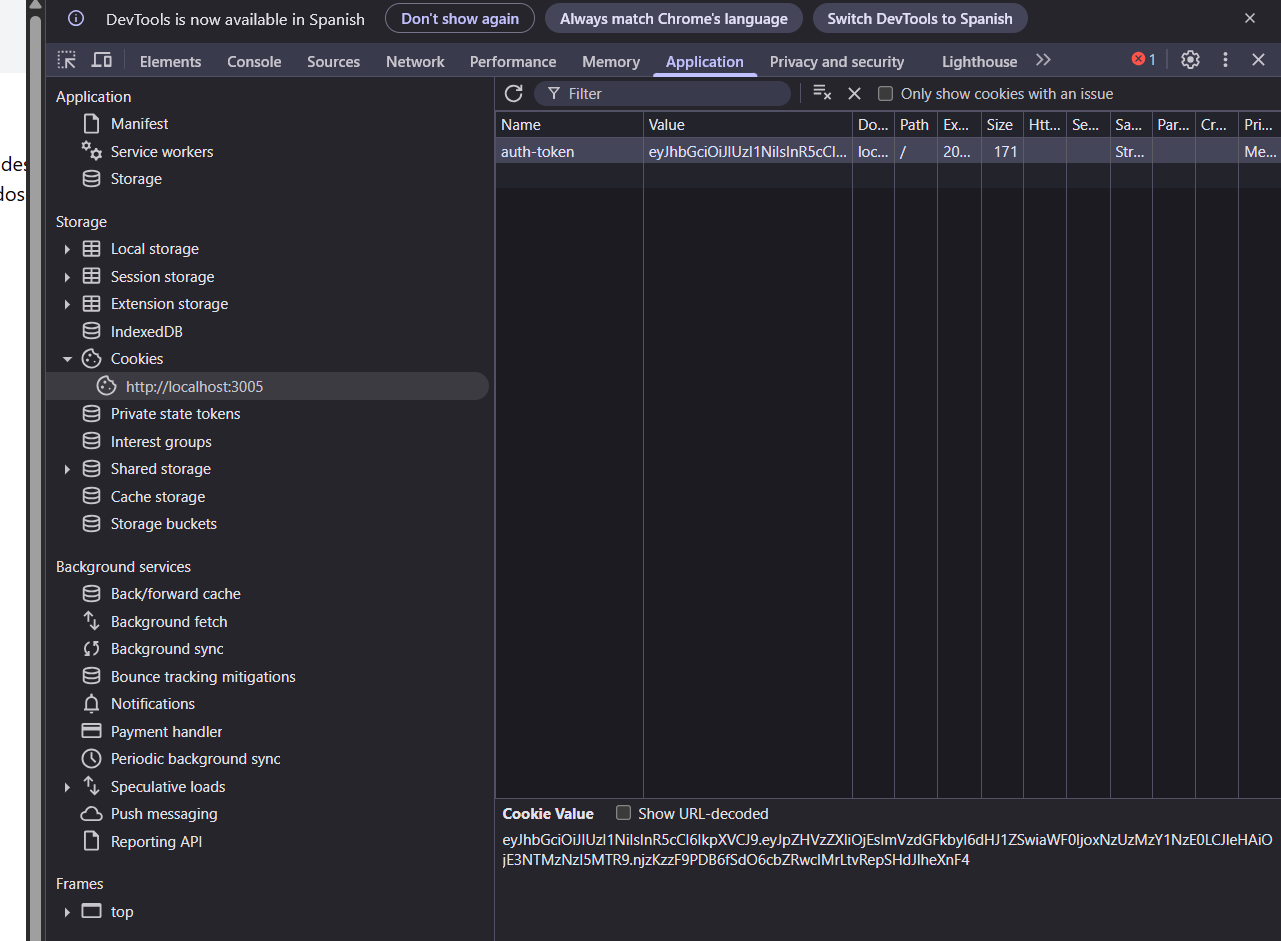
\includegraphics[width=0.8\textwidth]{assets/imagenes/bd.png}
    \label{fig:db} 
\end{figure} 
\FloatBarrier

\begin{figure}[!htb] 
    \centering 
    \caption{Diagrama de la base de datos} 
    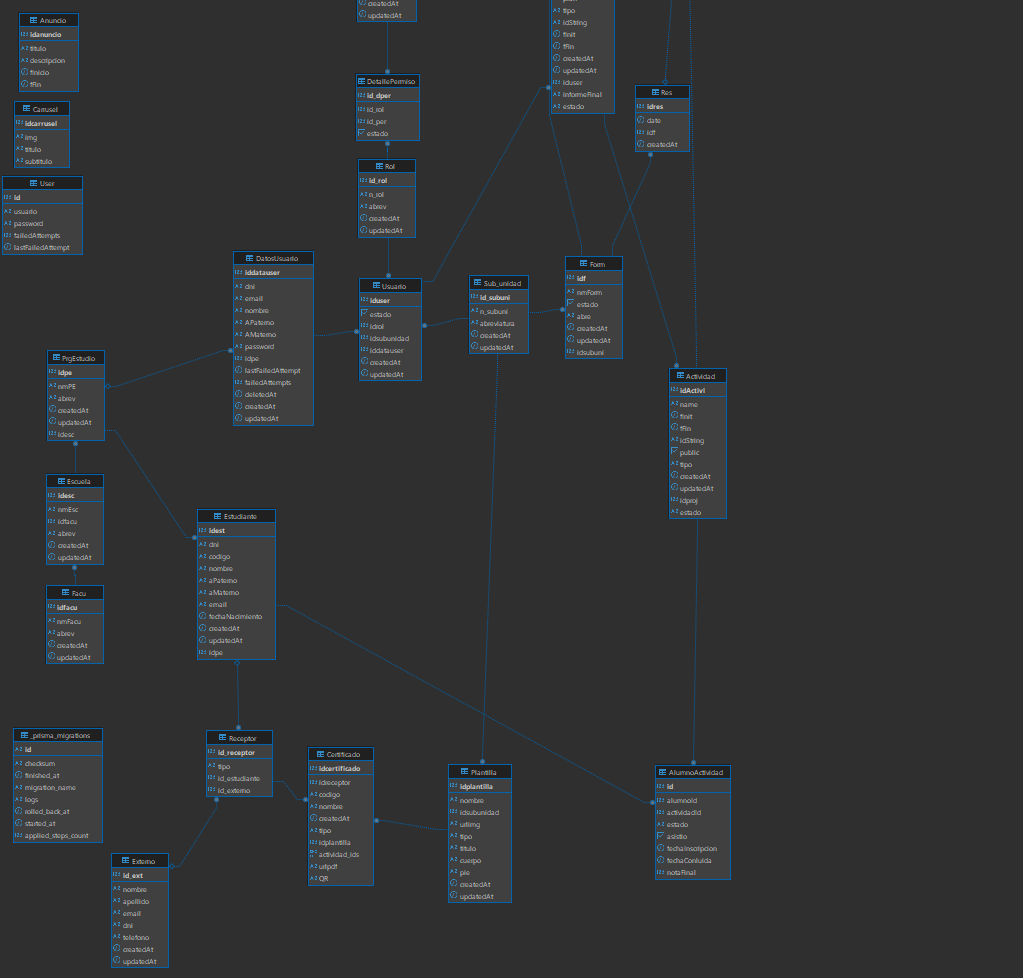
\includegraphics[width=0.8\textwidth]{assets/imagenes/diagrama.png}
    \label{fig:diagrama} 
\end{figure} 
\FloatBarrier

\begin{figure}[!htb] 
    \centering 
    \caption{Verificacion de cifrado} 
    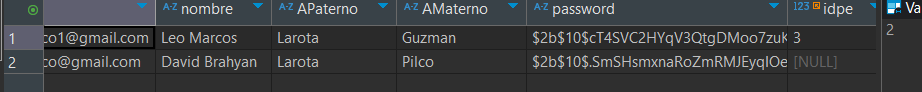
\includegraphics[width=0.8\textwidth]{assets/imagenes/cifrado.png}
    \label{fig:cifrado} 
\end{figure} 
\FloatBarrier

\section{Conclusiones}
El trabajo se desarrolló mediante un flujo iterativo e incremental por funcionalidad: se diseñó cada propuesta, se presentó al supervisor o encargado de la oficina, se implementó y se ajustó con base en la retroalimentación. Este flujo es compatible con prácticas asociadas a Scrum y XP, sin implicar la adopción completa de un marco formal. Se completaron al 100\% los requerimientos y el backend; el diseño y el frontend alcanzaron un 90\%, y las pruebas un 40\%. Los resultados muestran un sistema funcional y evidencian la necesidad de completar los componentes pendientes.
\section{Recomendaciones}
Para concluir el plan, se recomienda: 1) completar el 10\% pendiente del diseño y del frontend mediante la revisión de las funcionalidades; 2) completar el 60\% pendiente de las pruebas unitarias, de integración y de seguridad; y 3) mantener la presentación de cada funcionalidad al supervisor o encargado para incorporar la retroalimentación en los ajustes finales.

\newpage
\section{Anexos}
\section{Carta de presentación}

\includepdf[pages=-]{anexos/carta.pdf}

\section{Carta de aceptación}
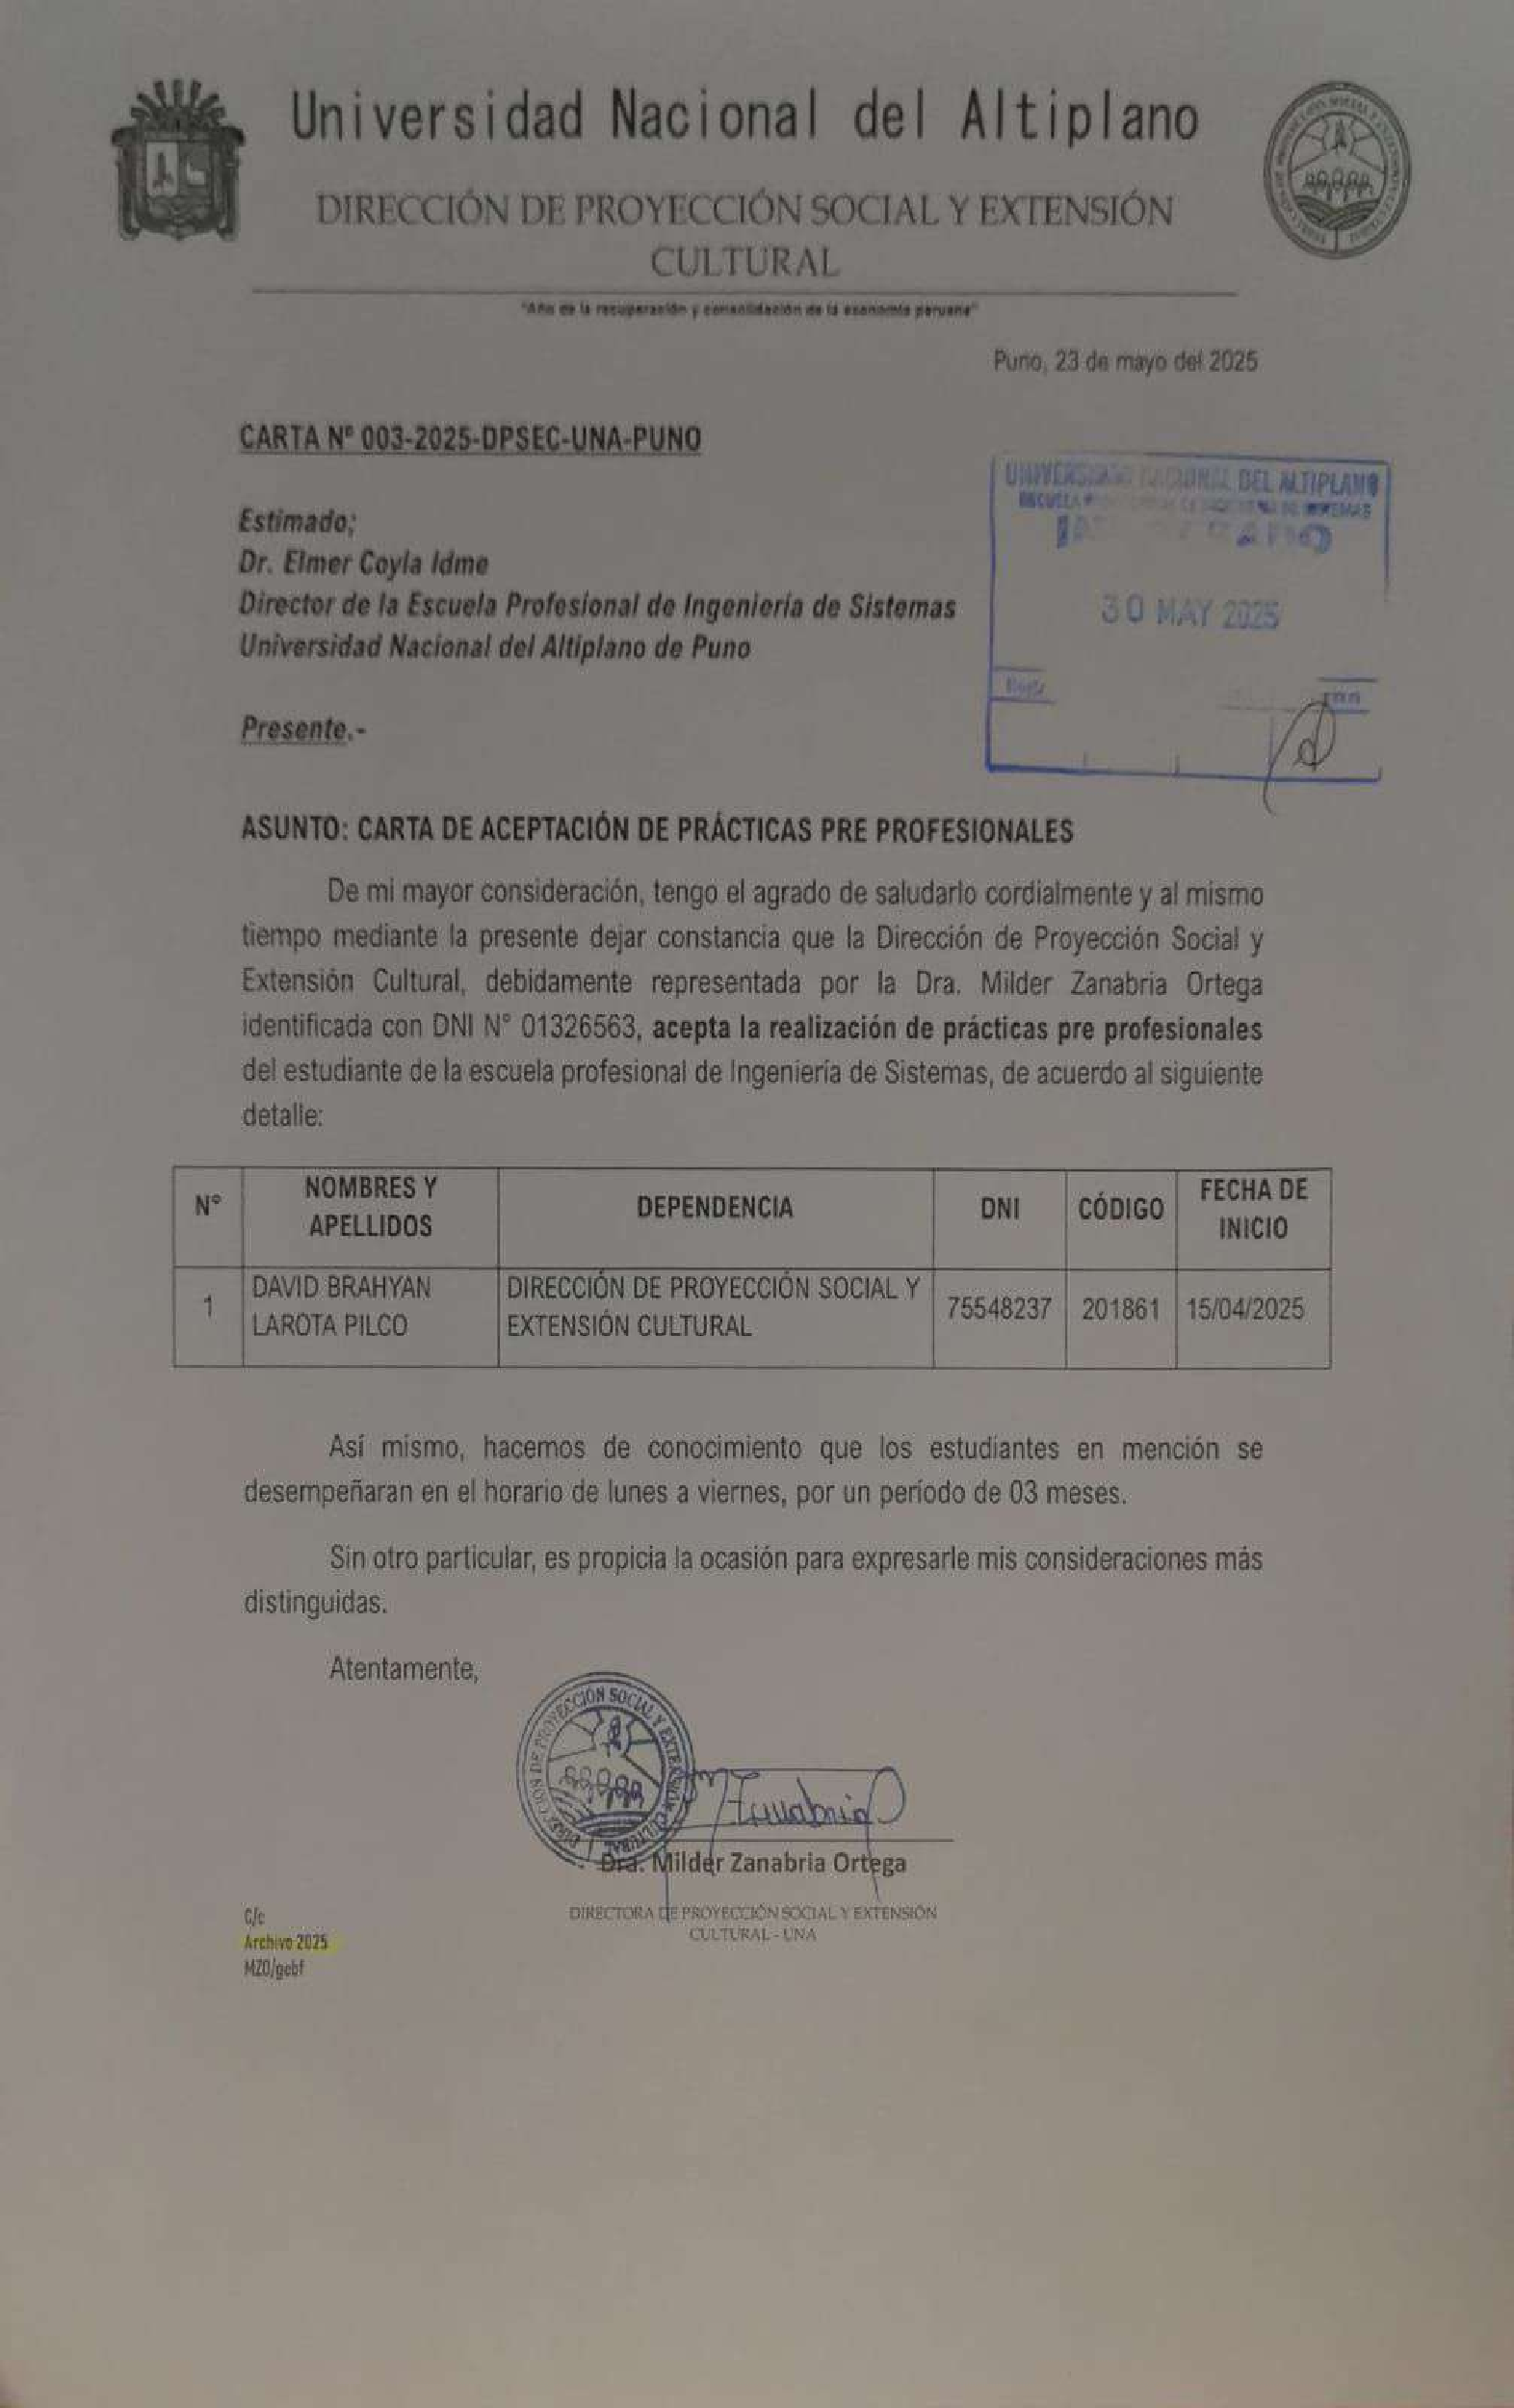
\includepdf[pages=-]{anexos/aceptacion.pdf}

\section{Evidencias de las prácticas: reuniones}
\begin{figure}[!htb] 
    \centering 
    \caption{Evidencia de las reuniones} 
    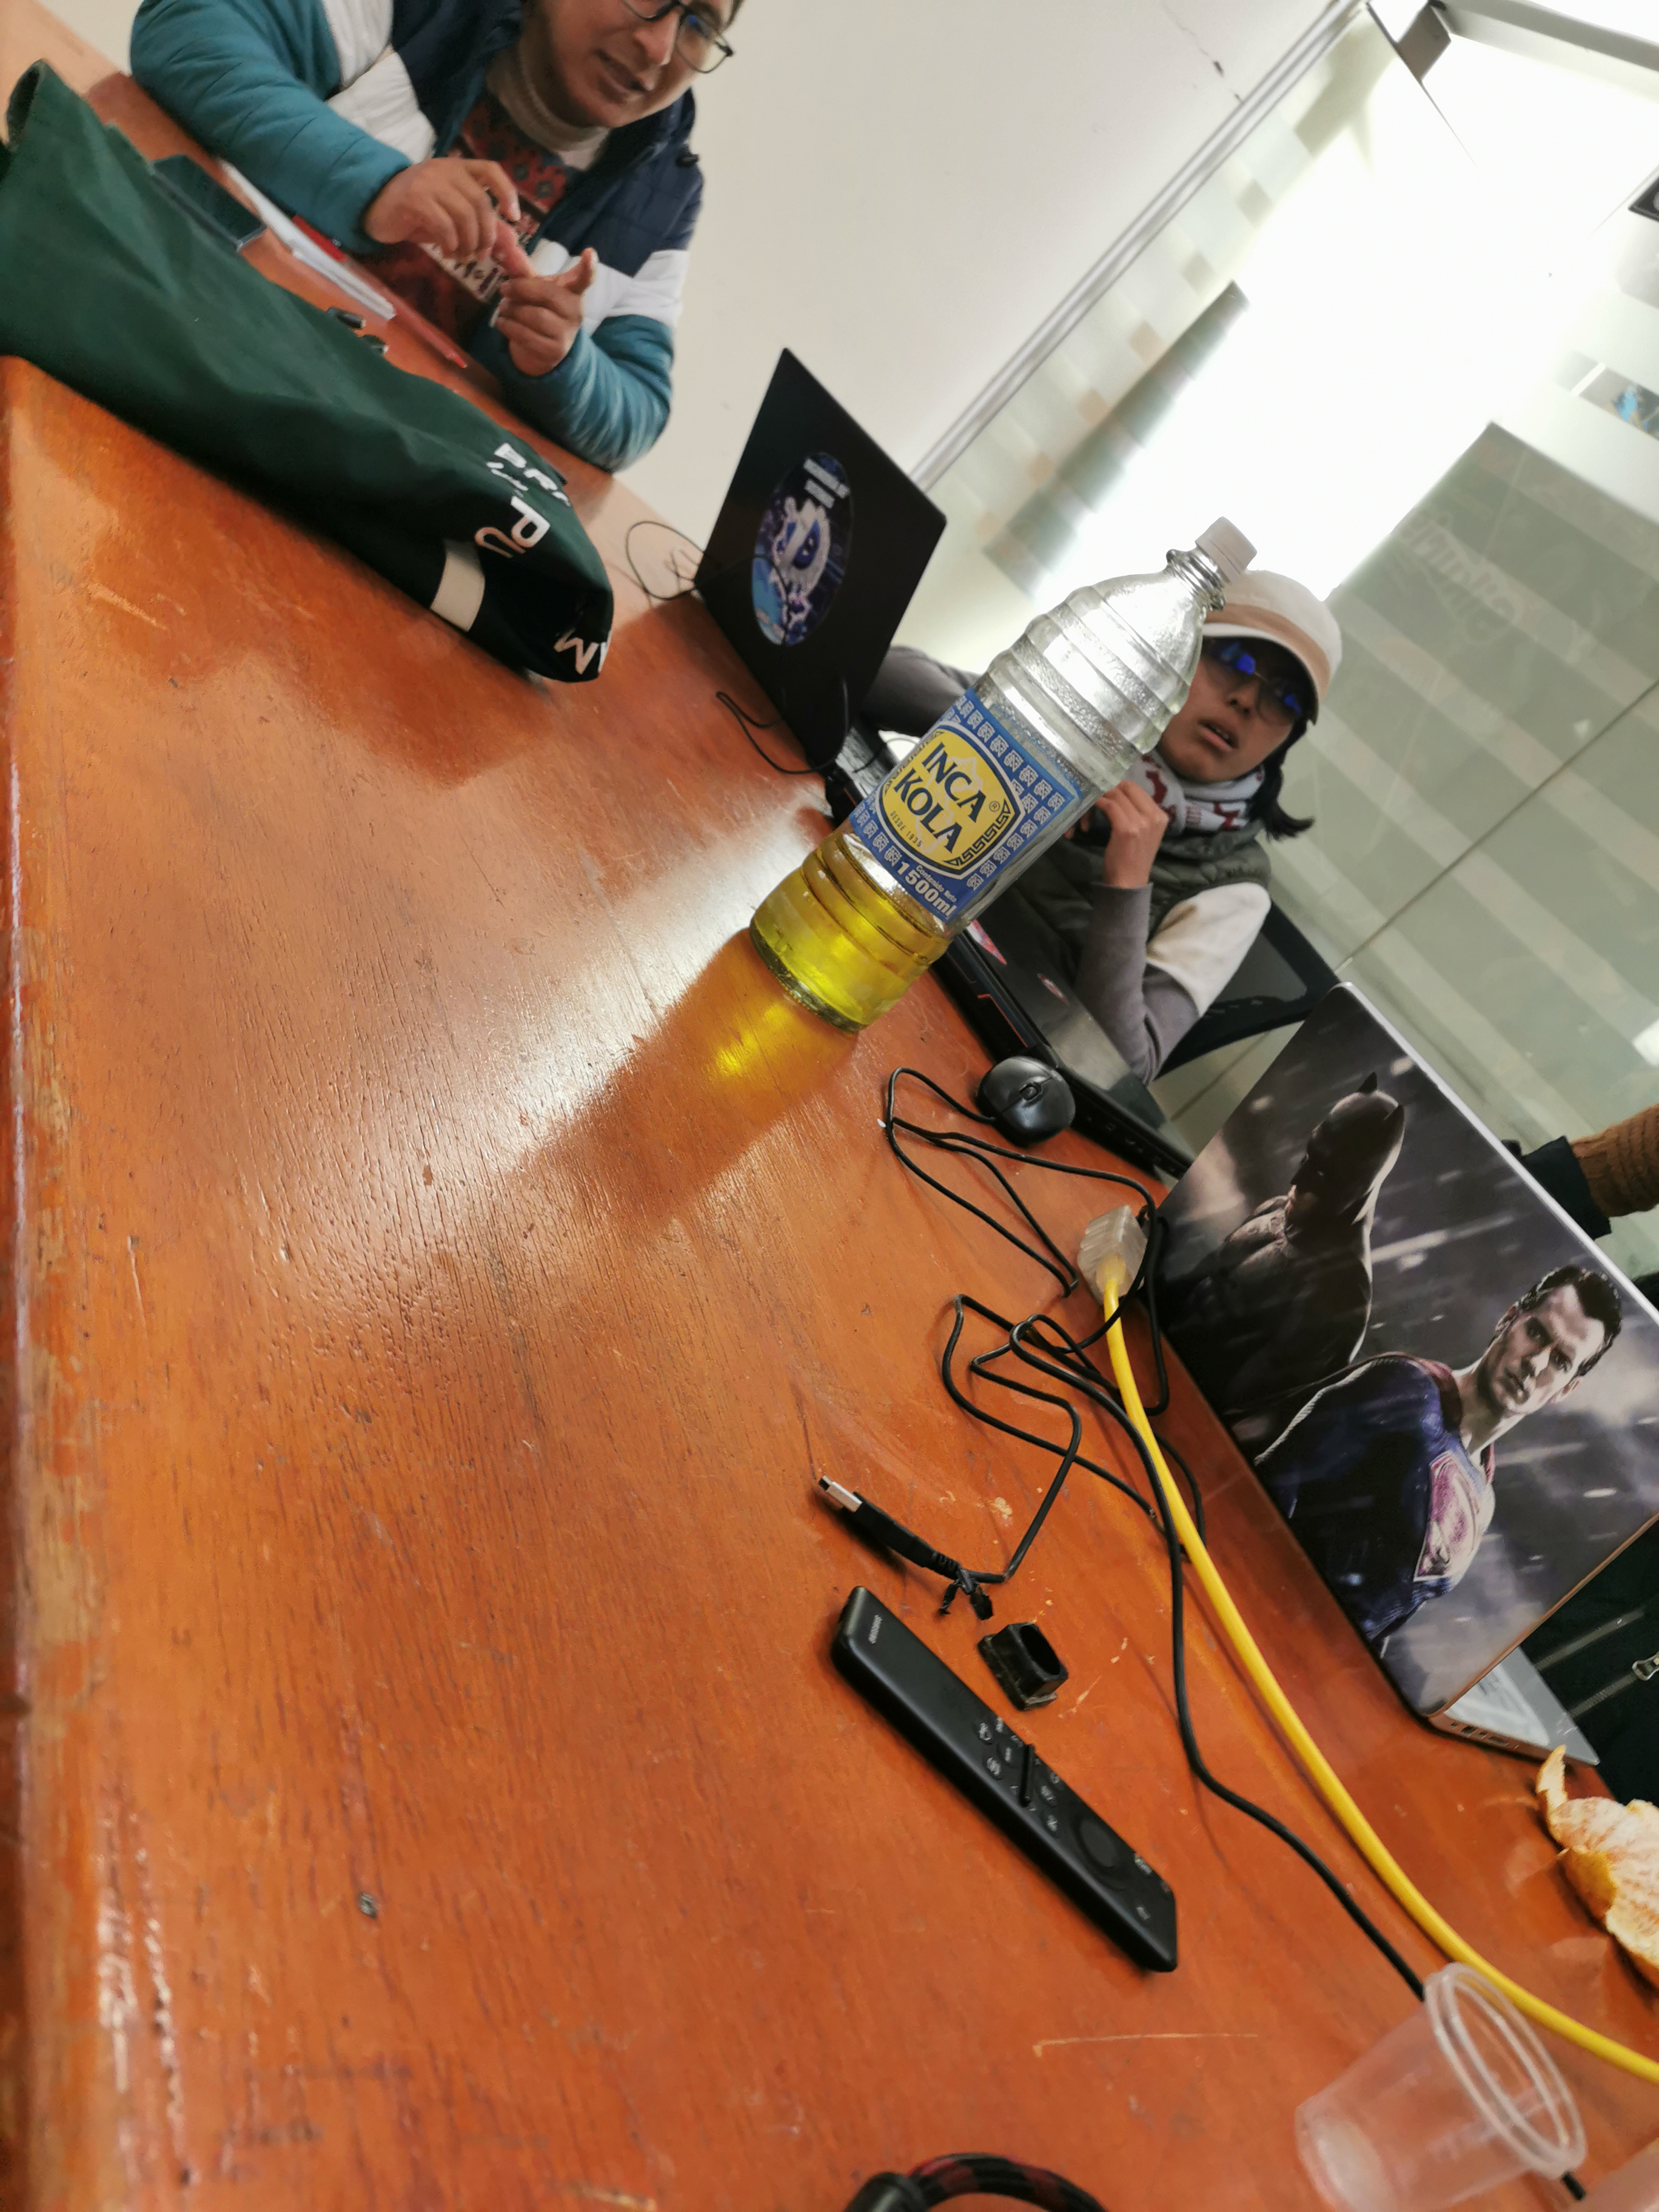
\includegraphics[width=0.8\textwidth]{assets/imagenes/practicas.jpg}
    \label{fig:reunion} 
\end{figure} 
\FloatBarrier
\begin{figure}[!htb] 
    \centering 
    \caption{Evidencia de las reuniones 1} 
    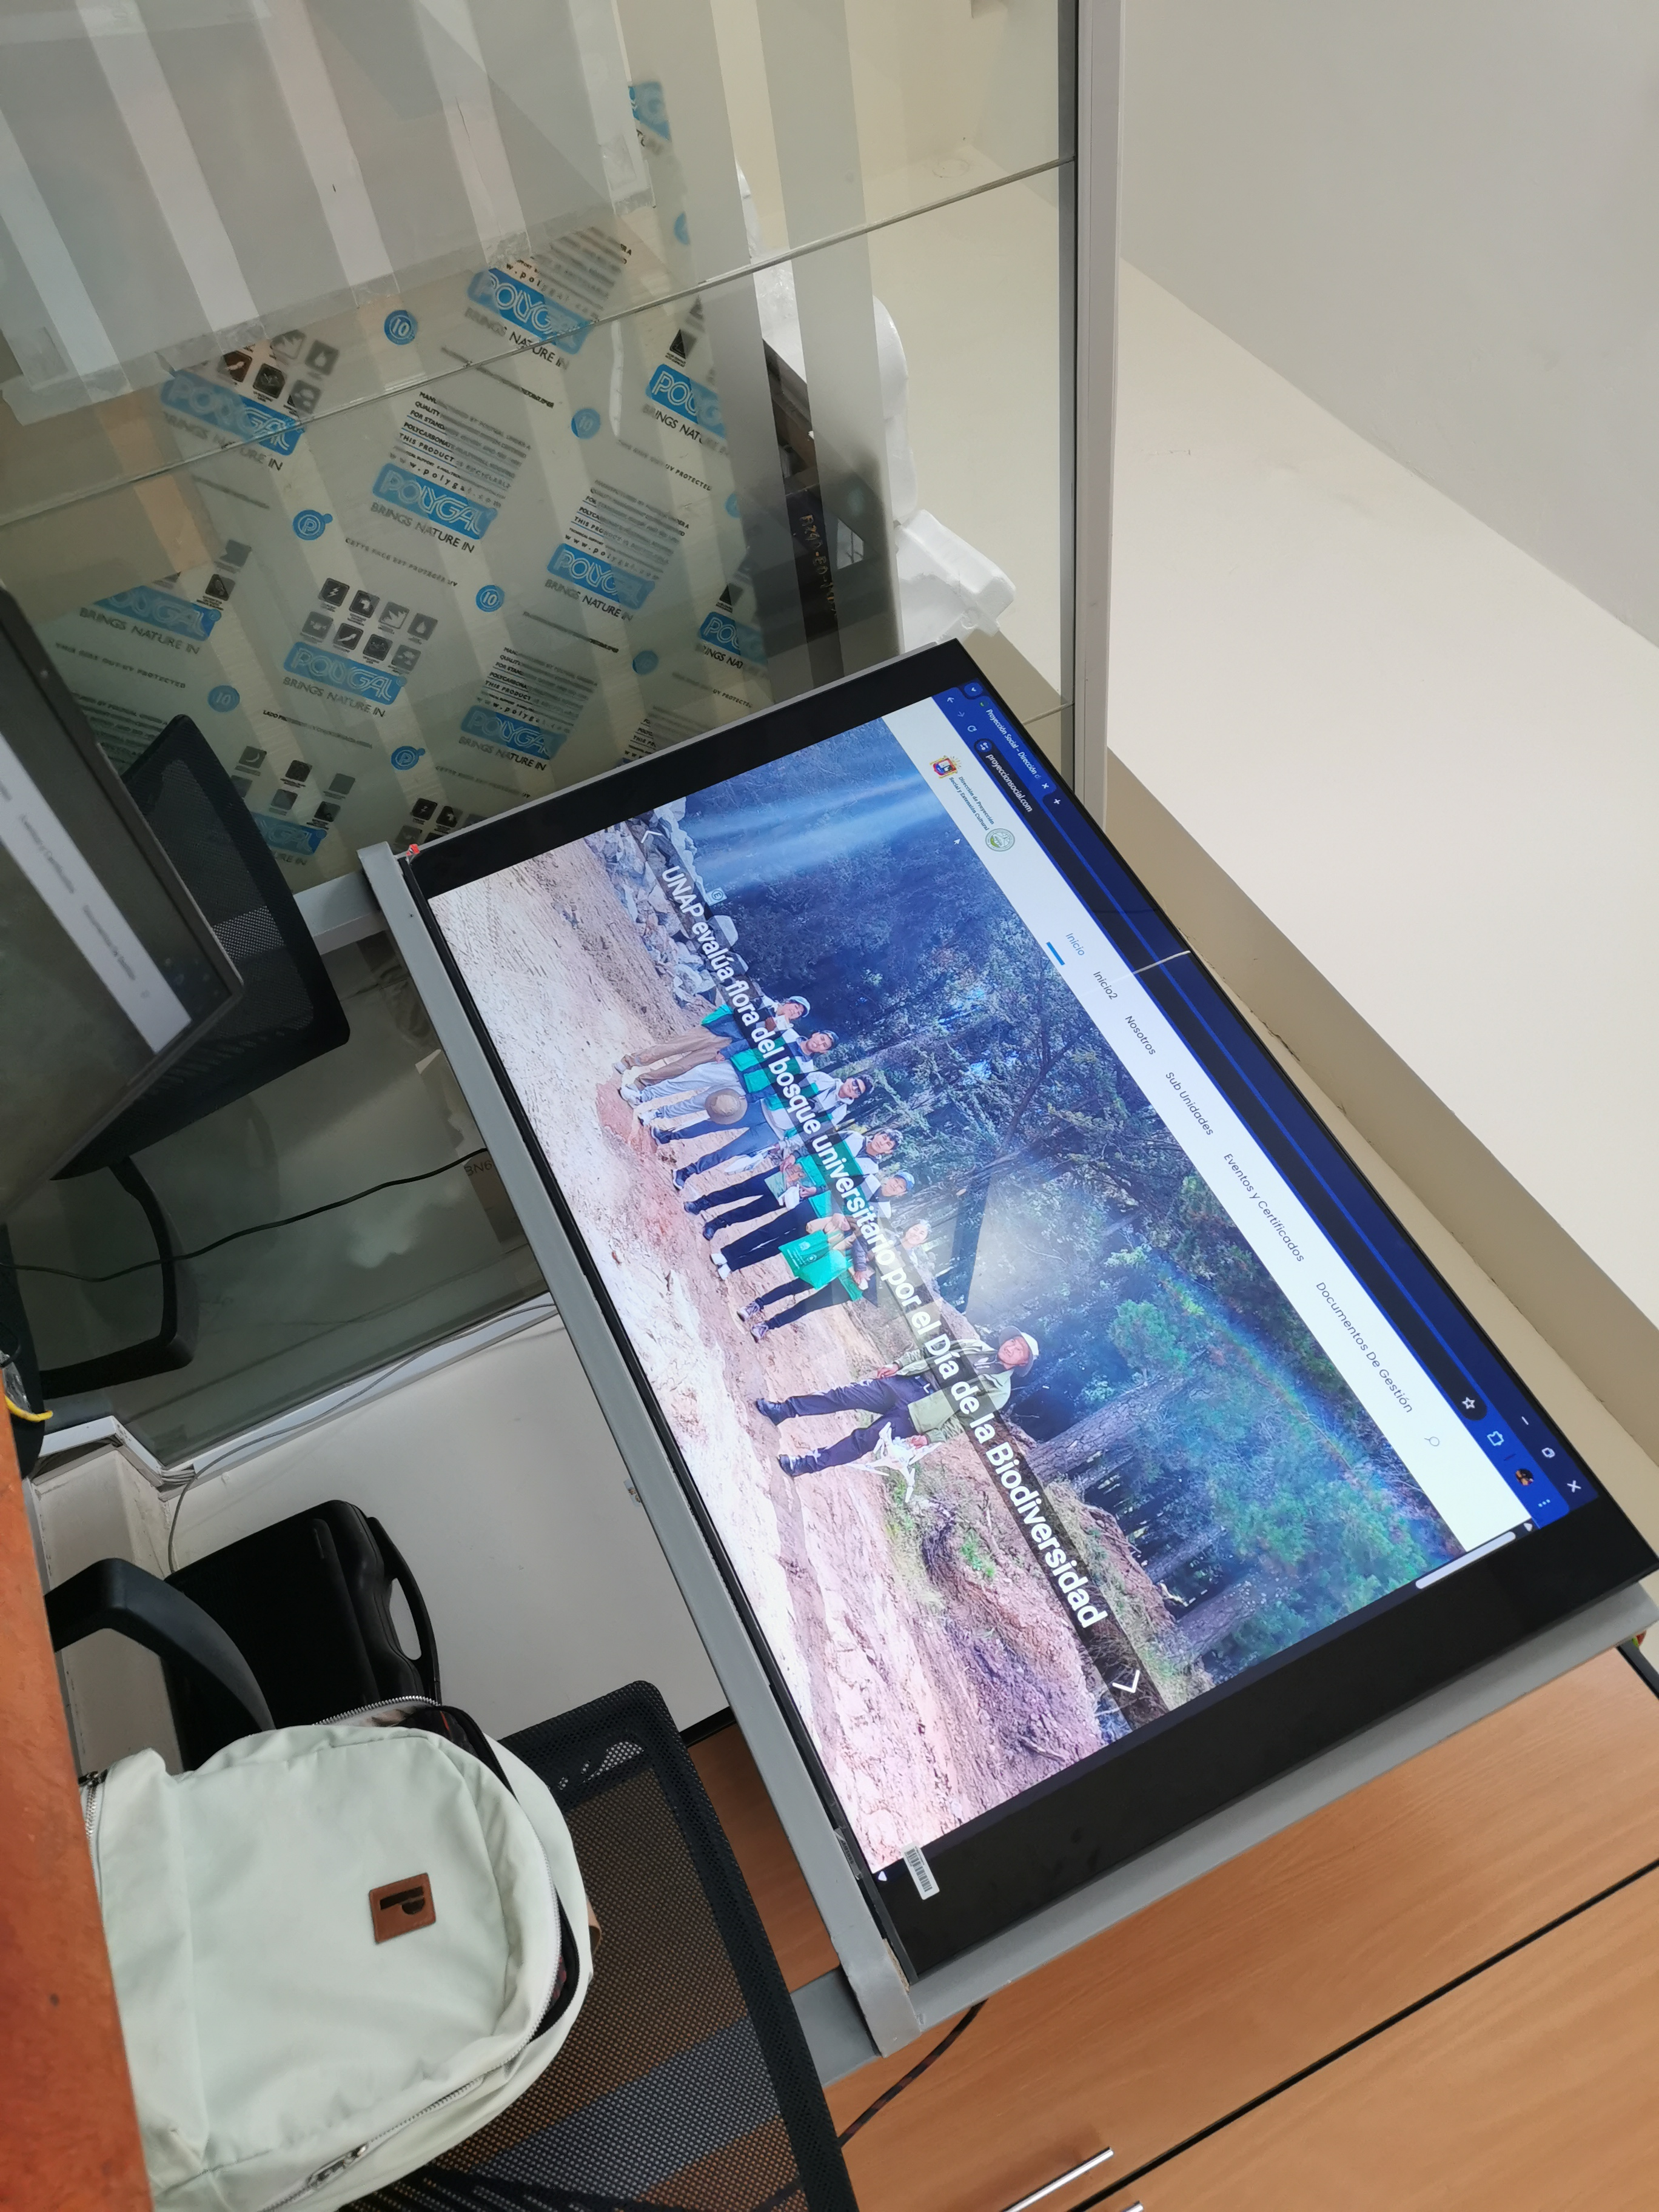
\includegraphics[width=0.8\textwidth]{assets/imagenes/practicas1.jpg}
\end{figure} 
\FloatBarrier

\begin{figure}[!htb] 
    \centering 
    \caption{Evidencia de las reuniones 2} 
    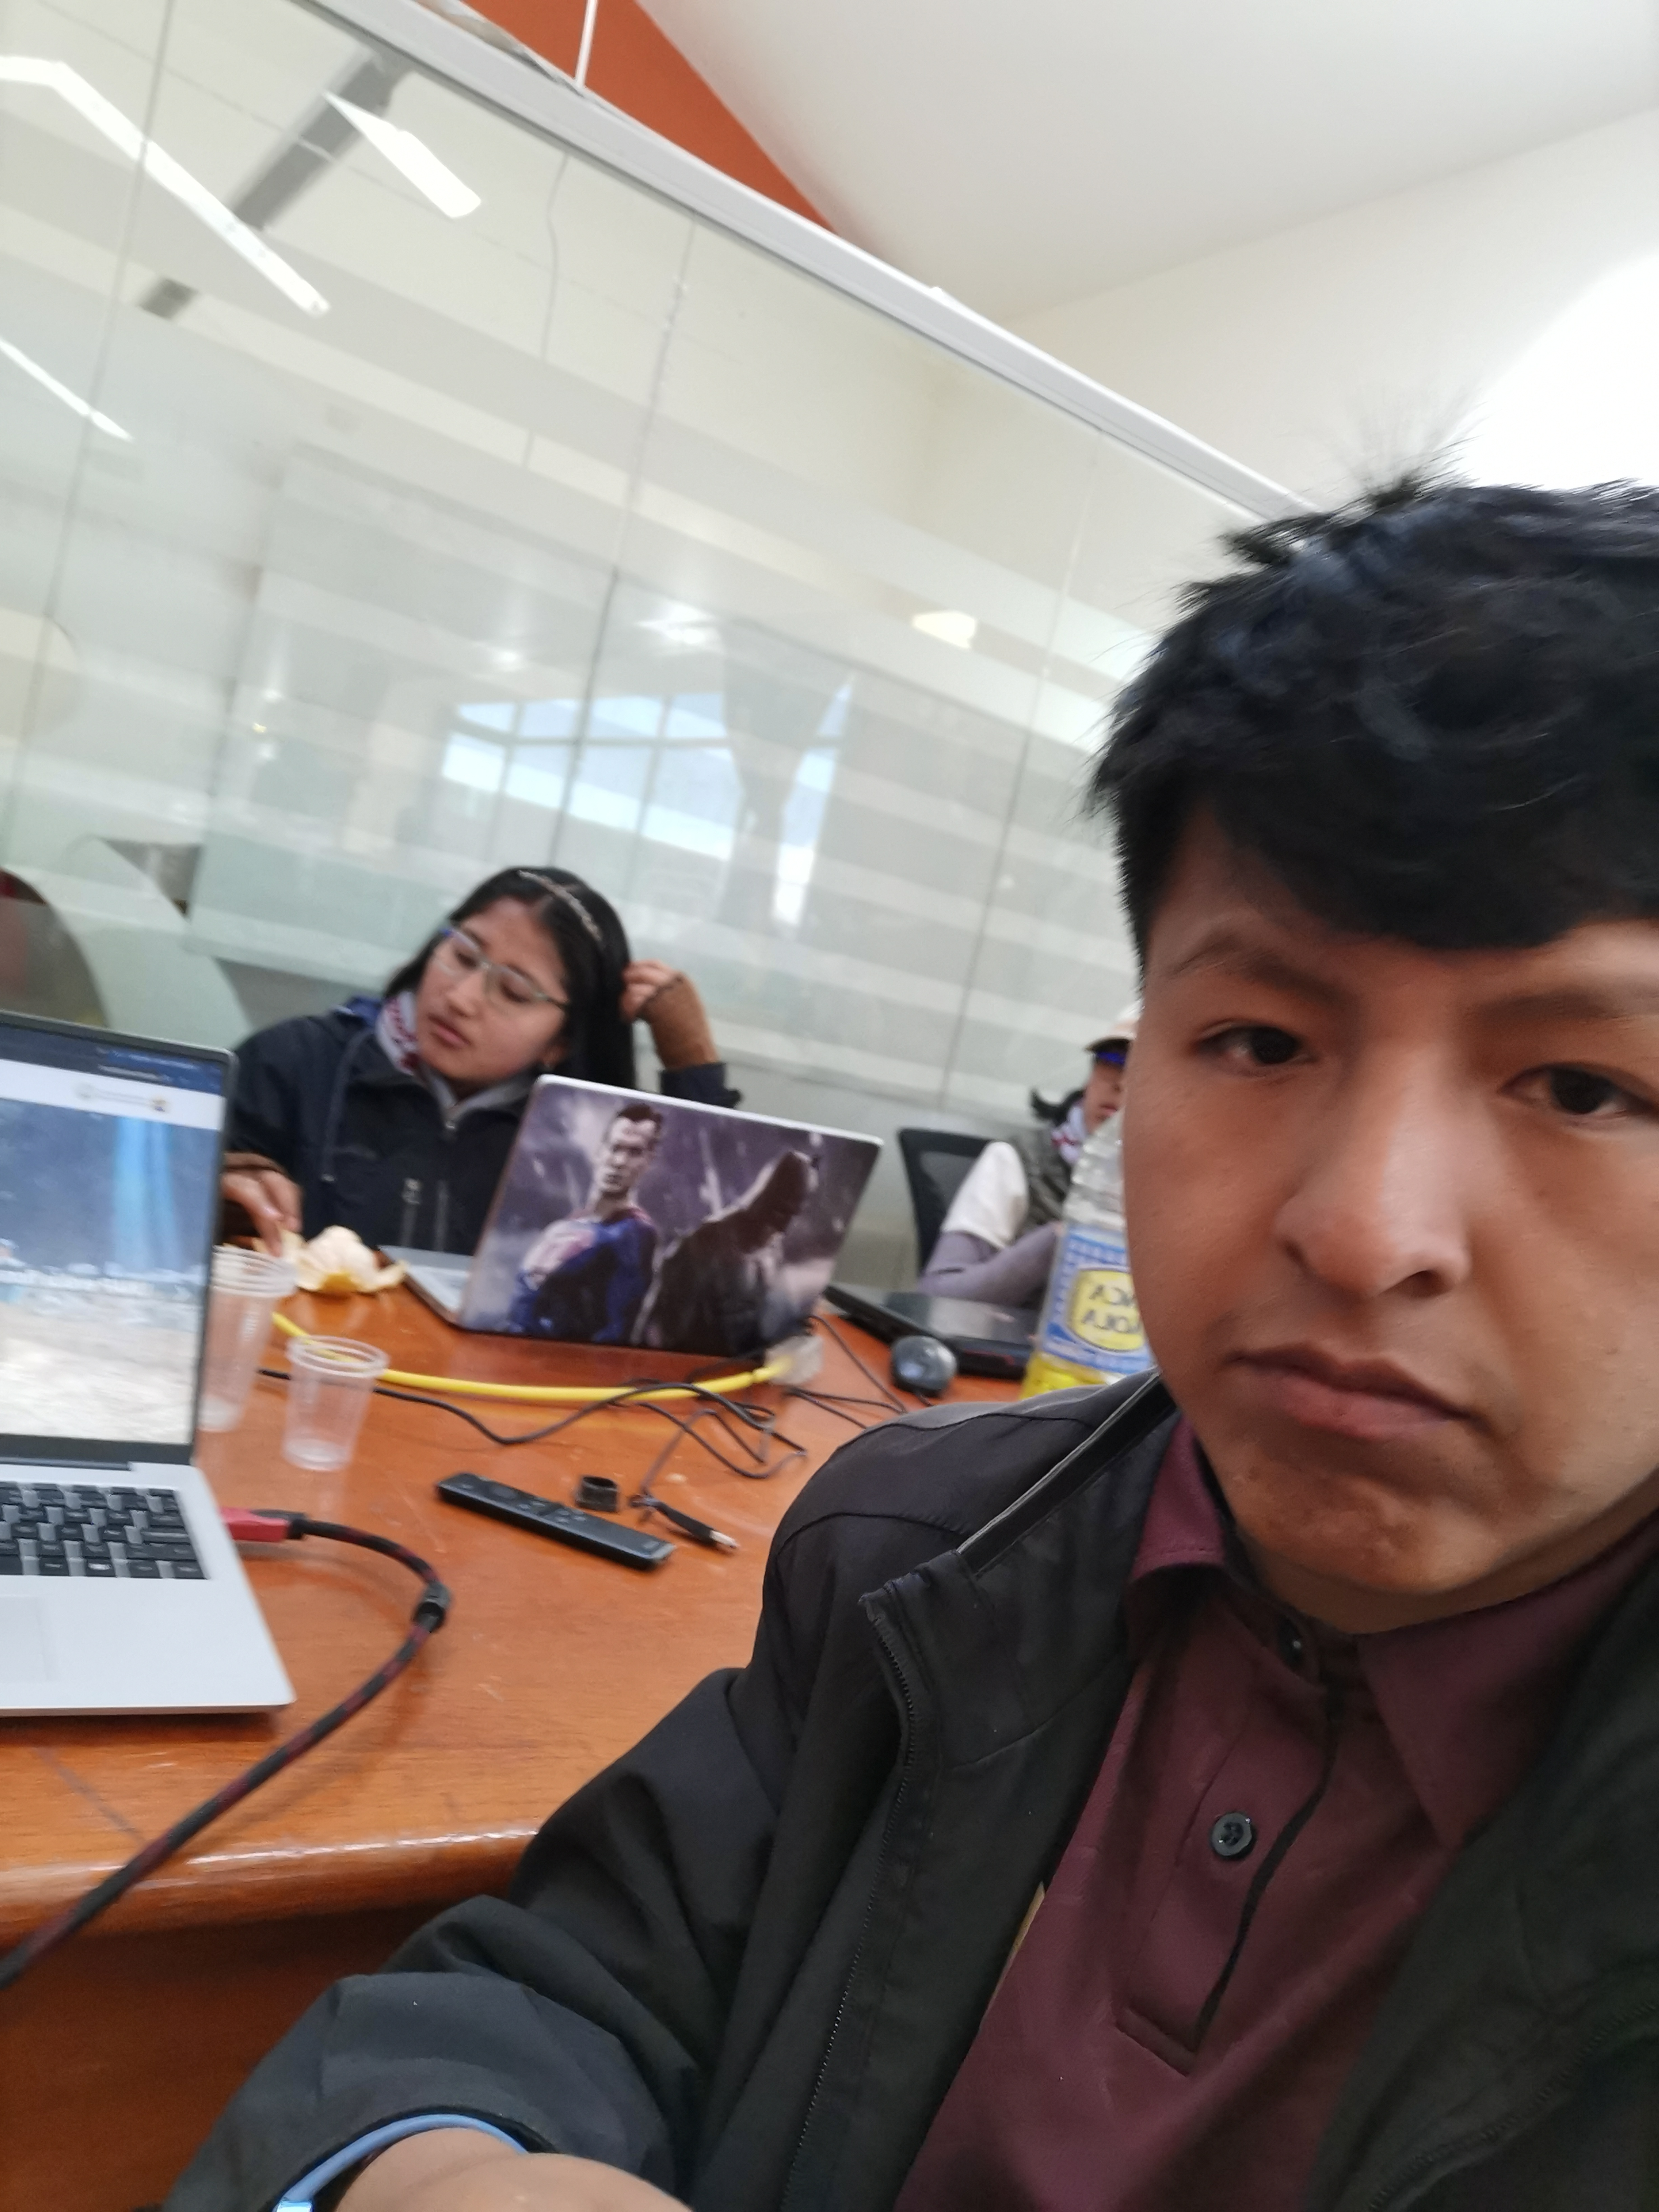
\includegraphics[width=0.8\textwidth]{assets/imagenes/practicas2.jpg}
\end{figure} 
\FloatBarrier

\section{Plan de practicas}

\includepdf[pages=-]{anexos/plan.pdf}  % Incluye todas las páginas de plan.pdf

%\FloatBarrier
%
%\section{Conclusión}
%\cite{prueba}
% 
%\newpage
%\renewcommand{\acronymname}{Abreviaciones} 
%\printglossaries
%
%\newpage
%\addtocounter{section}{1} % Incrementar el contador de secciones en 1
%\renewcommand{\refname}{\thesection \hspace{0.5em}  Referencias}
%
%\bibliographystyle{apacite}
%\bibliography{referencias/referencias.bib}


\end{document}
